\chapter{Tool demonstration for lifetime-long depletion: Transatomic Power MSR}

This chapter presents a validation demonstration applying SaltProc v1.0 to 
the \gls{TAP} \gls{MSR}. The \gls{TAP} concept was selected because it is well 
analyzed in the literature \cite{betzler_two-dimensional_2017, 
betzler_assessment_2017-1}; thus, code-to-code verification with 
ChemTRITON/SCALE is possible \cite{betzler_assessment_2017-1}. This chapter 
presents the \gls{TAP} \gls{MSR} core lifetime-long (25 years) depletion 
simulation with moderate time resolution (3-day depletion step) and at 
constant, 100\% power level. The results obtained with SaltProc v1.0 are 
compared with recent efforts discussed in Chapter 1, more specifically with 
full-core \gls{TAP} depletion analysis with assumed ideal removal efficiency 
(100\% of target isotope is removed) by Betzler \emph{et al.} 
\cite{betzler_assessment_2017-1}. This validation effort 
showed that SaltProc v1.0 solution is correct for the case with \emph{ideal 
extraction efficiency}. 

Finally, this chapter presents lifetime-long fuel salt depletion simulation 
for the case with \emph{realistic, physics-based} mathematical model for noble 
gas removal efficiency which provides fuel isotopic composition evolution 
during 25 years of the \gls{TAP} \gls{MSR} operation. Detailed insights about 
fuel salt composition and neutron spectrum dynamics obtained herein will be 
used in the following chapters to investigate the \gls{TAP} reactor poisoning 
during load-following and safety parameters evolution during operation.


\section{Transatomic Power Molten Salt Reactor design 
description}\label{sec:tap_design_sum}

The \gls{TAP} concept is a 1250 MW$_{th}$ \gls{MSR} with a LiF-based uranium 
fuel salt \cite{transatomic_power_corporation_technical_2016}. This concept 
uses configurable zirconium hydride rods as the moderator while most \gls{MSR} 
designs typically propose high-density reactor graphite. Zirconium hydride 
offers a much higher neutron moderating density than graphite: much less 
zirconium hydride volume is needed to achieve a thermal energy spectrum 
similar to one obtained with graphite moderator. Moreover, zirconium hydride 
has a much longer lifespan in extreme operational conditions (high 
temperature, large neutron flux, chemically aggressive salt) than reactor 
graphite. Finally, zirconium hydride is a nonporous material and holds up 
fewer neutron poisons (e.g., xenon, krypton) than does high-density 
reactor graphite.

In this section, the design characteristics and reprocessing plant design are 
based on information presented in the TAP white papers  
\cite{transatomic_power_corporation_technical_2016,
transatomic_power_corporation_neutronics_2016} and \gls{ORNL} technical 
reports \cite{betzler_two-dimensional_2017, betzler_assessment_2017-1}.

\subsection{General design description}

Figure~\ref{fig:tap-rendering} demonstrates a rendering of the primary and 
secondary loop of the \gls{TAP} \gls{MSR} seated inside a concrete nuclear 
island. Figure~\ref{fig:tap-primary-scheme} shows the schematic design of a 
520 MW$_{e}$, 2-loop nuclear reactor system with an intermediate salt loop.
\begin{figure}[h] % replace 't' with 'b' to 
	\centering
	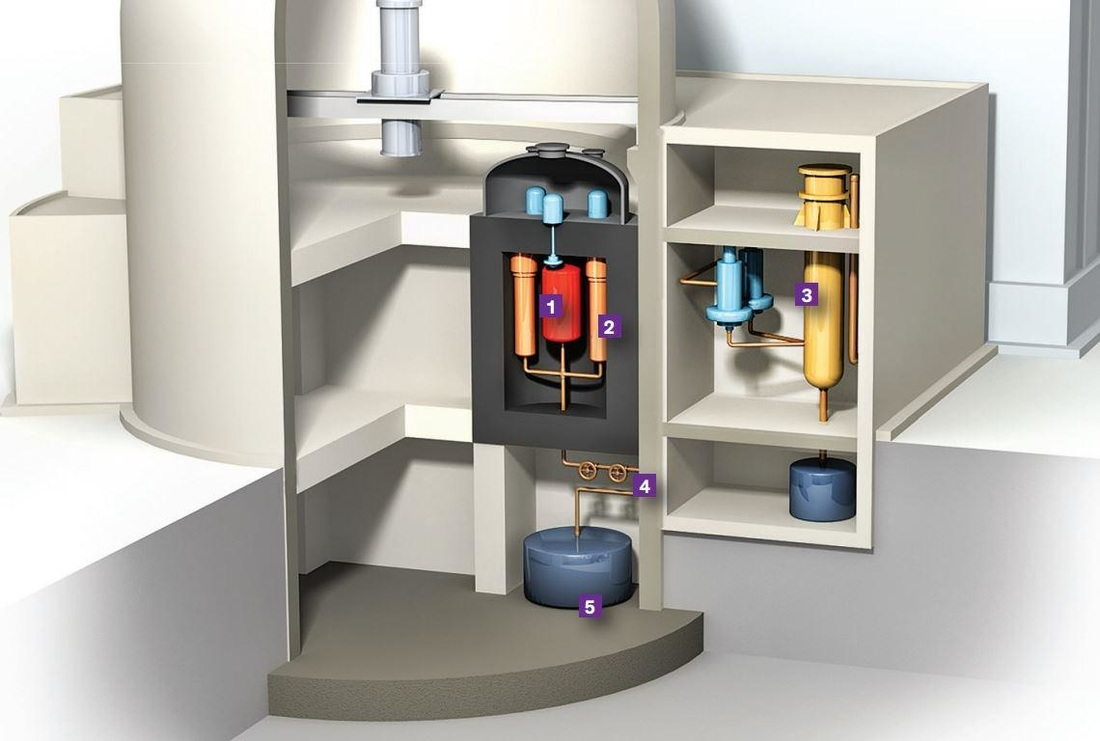
\includegraphics[width=\textwidth]{ch4/tap_render.jpg}
	\caption{Rendering of the \gls{TAP} \gls{MSR}. The fission happens in the 
		fuel salt inside the reactor vessel (1). The heat generated by 
		self-sustaining nuclear fission reaction would be transferred to the 
		secondary salt by heat exchanger (2), which would boil water in the 
		steam 
		generator (3). Valves made of salt with higher melting point (4) would 
		melt in case of emergency, allowing the salt to drain into a drain 
		tank 
		(5) which is able to passively dissipate decay heat	(reproduced from 
		\cite{strickland_transatomic_2014}, illustration by Emily Cooper).}
	\label{fig:tap-rendering}
\end{figure}
\begin{figure}[h] % replace 't' with 'b' to 
	\centering
	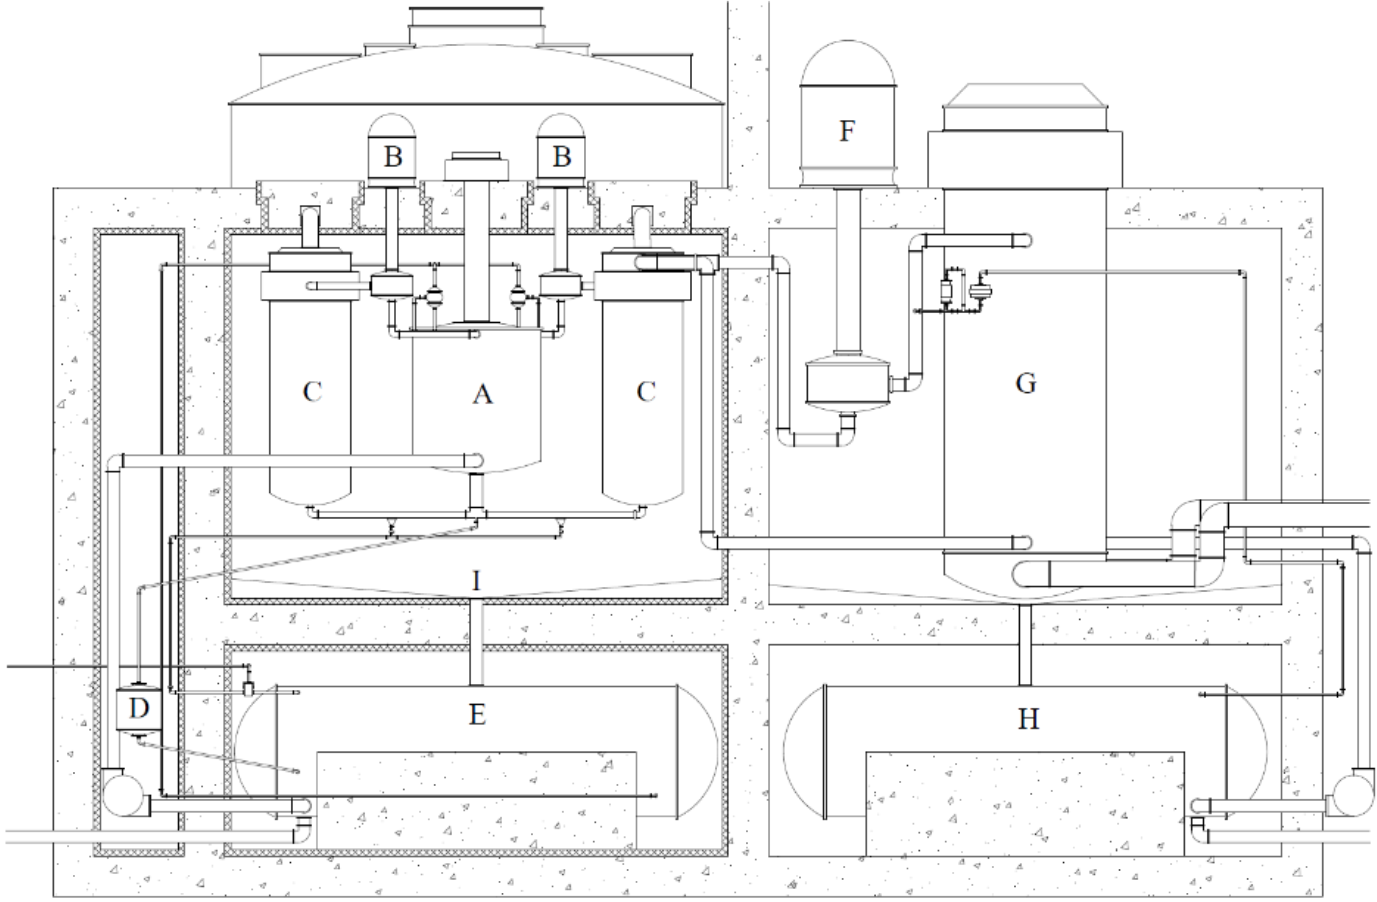
\includegraphics[width=\textwidth]{ch4/tap_simplified_scheme.png}
	\caption{Simplified schematic of the \gls{TAP} \gls{MSR} primary and  
		secondary loops (reproduced from the Transatomic Power Technical White 
		Paper \cite{transatomic_power_corporation_technical_2016}). Figure 
		legend: 
		A) reactor vessel, b) fuel salt pumps, C) primary heat exchangers, D) 
		freeze plug, E) primary loop drain tank, F) secondary loop salt pump, 
		G) 
		steam generator, H) secondary loop drain tank, I) fuel catch basin.}
	\label{fig:tap-primary-scheme}
\end{figure}

The \gls{TAP} design (figure~\ref{fig:tap-side-view}) is very similar to 
original \gls{MSRE} design developed by \gls{ORNL} 
\cite{haubenreich_experience_1970} but has two major innovations: 
the fuel salt composition and the moderator. The \gls{MSRE}'s 
LiF-BeF$_2$-ZrF$_4$-UF$_4$ salt has been substituted with LiF-UF$_4$ salt 
which allows for an increase in the uranium concentration within the fuel salt 
from 0.9 to 27.5\% while maintaining a relatively low melting point 
(490$^{\circ}$C compared with 434$^{\circ}$C for the original \gls{MSRE}'s 
salt) \cite{betzler_two-dimensional_2017}. The graphite has a very high 
thermal scattering cross section which makes it a perfect moderator but has 
a few major drawbacks: 
\begin{enumerate}[label=(\alph*), itemsep=-1ex]
	\item low lethargy gain per collision requires a large volume of 
	moderator to be present to reach criticality, which leads to a larger core 
	and obstructs the core power density;
	\item even special reactor-grade graphite has relatively high porosity, 
	consequently, it holds gaseous \glspl{FP} (e.g., tritium, xenon) in pores;
	\item reactor graphite lifespan in a commercial reactor is 
	approximately 10 years \cite{robertson_conceptual_1971}.
\end{enumerate}
As previously mentioned, to resolve these issues, the \gls{TAP} concept uses 
zirconium hydride instead of graphite, allowing for a more compact core and a 
significant increase in power density. These two innovative design choices, 
together with a configurable moderator (the moderator-to-fuel ratio can be 
changed during operation), facilitate the deployment of this conceptual design 
in the current commercially available 5\% enriched \gls{LEU} fuel cycle. 
\begin{figure}[h] % replace 't' with 'b' to 
	\hspace{+2.2in}
	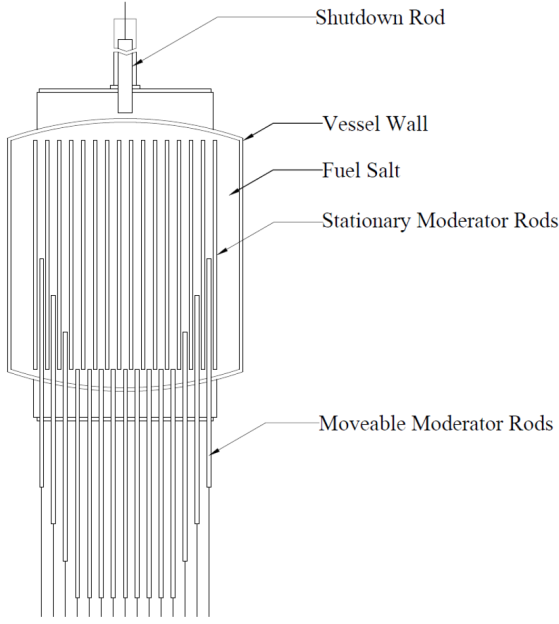
\includegraphics[width=0.65\textwidth]{ch4/tap_front_view.png}
	\caption{The \gls{TAP} \gls{MSR} schematic view showing movable moderator 
		rod bundles and shutdown rod (reproduced from Transatomic Power 
		White Paper \cite{transatomic_power_corporation_technical_2016}).}
	\label{fig:tap-side-view}
\end{figure}

The \gls{TAP} \gls{MSR} primary loop contains the reactor core volume  
(including the zirconium hydride moderator rods with silicon carbide  
cladding), pumps, and primary heat exchangers. Pumps circulate the  
LiF-(Act)F$_4$ fuel salt through the primary loop. The pumps, vessels, tanks, 
and piping are made of a nickel-based alloy (similar to Hastelloy-N\footnote{ 
Hastelloy-N is very common in \gls{MSR} designs now, but was developed at 
\gls{ORNL} in the \gls{MSRE} program that started in the 1950s.}), which 
is highly resistant to corrosion in various molten salt environments. Inside 
the reactor vessel, near the zirconium hydride moderator rods, the fuel salt 
is in a critical configuration and generates heat. Table~\ref{tab:tap_tab} 
contains details of the \gls{TAP} system design which are taken from technical 
white paper \cite{transatomic_power_corporation_technical_2016} and a 
neutronics overview \cite{transatomic_power_corporation_neutronics_2016} as 
well as \gls{ORNL} analysis of the \gls{TAP} design 
\cite{betzler_two-dimensional_2017, betzler_assessment_2017-1}. 
%%%%%%%%%%%%%%%%%%%%%%%%%%%%%%%%%%%%%%%%
\begin{table}[h!]
	\caption{Summary of principal data for the \gls{TAP} \gls{MSR} 
		(reproduced from \cite{betzler_assessment_2017-1, 
		transatomic_power_corporation_technical_2016}). }
		\centering
	\begin{tabularx}{0.8\textwidth}{L R}
		\hline
		Thermal power   		& 1250 MW$_{th}  $       		\\ 
		Electric power		    & 520 MW$_e  $ 			 		\\ 
		Gross thermal efficiency& 44\%     				 		\\  
		Outlet temperature      & 620$^{\circ}$C         		\\ 
		Fuel salt components    & LiF-UF$_4$				    \\  
		Fuel salt composition   & 72.5-27.5 mole\%				\\  
		Uranium enrichment      & 5\% $^{235}$U          	    \\
		Moderator               & Zirconium Hydride (ZrH$_{1.66}$) rods \\
								& (with silicon carbide cladding)       \\
		Neutron spectrum at the \gls{BOL} & intermediate \\
		\qquad\qquad\qquad\qquad\space at the \gls{EOL}     & thermal      \\
		\hline
	\end{tabularx}
	\label{tab:tap_tab}
\end{table}
%%%%%%%%%%%%%%%%%%%%%%%%%%%%%%%%%%%%%%%%%%%%%%%%%%%%%%%%%%%%%%%%%%%%%%%%%%%%%%%

\subsection{Reactor core design}
In the \gls{TAP} core (Figure~\ref{fig:tap-core-ben}), fuel salt flows around 
moderator assemblies consisting of lattices of zirconium hydride rods clad in 
a corrosion-resistant silicone carbide. The \gls{TAP} reactor pressure vessel 
is a cylinder with an inner radius 150 cm, height 350 cm, and wall thickness 5 
cm made of a nickel-based alloy. 
\begin{figure}[t] % replace 't' with 'b' to 
	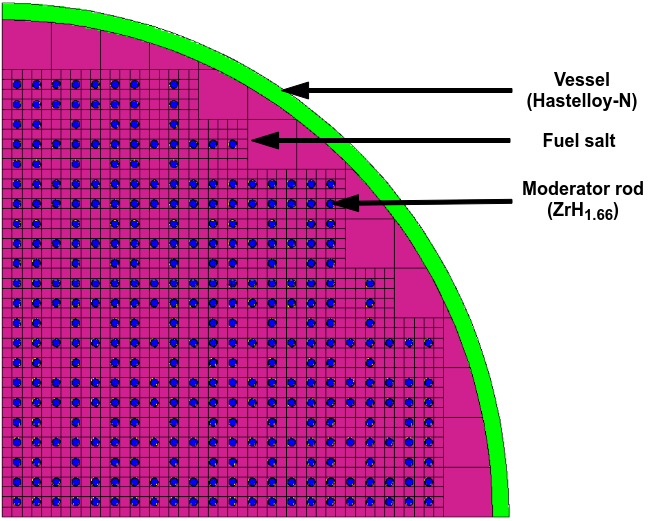
\includegraphics[width=\textwidth]{ch4/tap_core_ornl.png}
	\vspace{-0.35in}
	\caption{The \gls{TAP} \gls{MSR} schematic core view showing moderator 
		rods (reproduced from ORNL/TM-2017/475  
		\cite{betzler_assessment_2017-1}).}
	\label{fig:tap-core-ben}
\end{figure}

The \gls{SVF} in the core is parameter similar to wide-used moderator-to-fuel 
ratio and can be defined as:
\begin{align}
SVF &= \frac{V_F}{V_F+V_M} = \frac{1}{1+V_M/V_F}
\intertext{where}
V_F &= \mbox{the fuel volume $[m^3]$} \nonumber \\
V_M &= \mbox{the moderator volume $[m^3]$} \nonumber \\
V_M/V_F &= \mbox{the moderator-to-fuel salt ratio $[-]$.} \nonumber
\end{align}

Figure~\ref{fig:svf-predetermined} shows the \gls{SVF} variation during  
operation that shifts the reactor neutron energy spectrum from intermediate to 
thermal to maximize fuel burnup. At the \gls{BOL}, a high \gls{SVF} is 
selected to obtain relatively hard spectrum and enhance fertile material 
($^{238}$U) conversion into the fissile material ($^{239}$Pu) when the 
startup fissile material ($^{235}$U) inventory is still large. As fissile 
concentration in the fuel salt declines, an additional moderator are 
introduced to maintain criticality, leading to salt volume fraction decrease 
(see Figure~\ref{fig:svf-predetermined}).

Initial \gls{TAP} concept suggested vary salt volume fraction by inserting 
fixed-sized moderator rods via the bottom of the reactor vessel (for safety 
considerations), similarly to moving the control rods in a \gls{BWR}, as shown 
in Figure~\ref{fig:tap-side-view} 
\cite{transatomic_power_corporation_neutronics_2016}. The later \gls{TAP} 
concept proposes reducing the \gls{SVF} by reconfiguring the moderator rods 
during regular shutdown for reactor maintenance 
\cite{betzler_assessment_2017-1}. For the 
\gls{TAP} reactor, \gls{EOL} occurs when the maximum number of moderator rods 
are inserted into the core, and a further injection of fresh fuel salt does 
not alter criticality. Unmoderated salt is flowing in the annulus between the 
core, and the vessel wall provides for a potential reduction in fast neutron 
flux at the vessel structural material.
\begin{figure}[t] % replace 't' with 'b' to 
	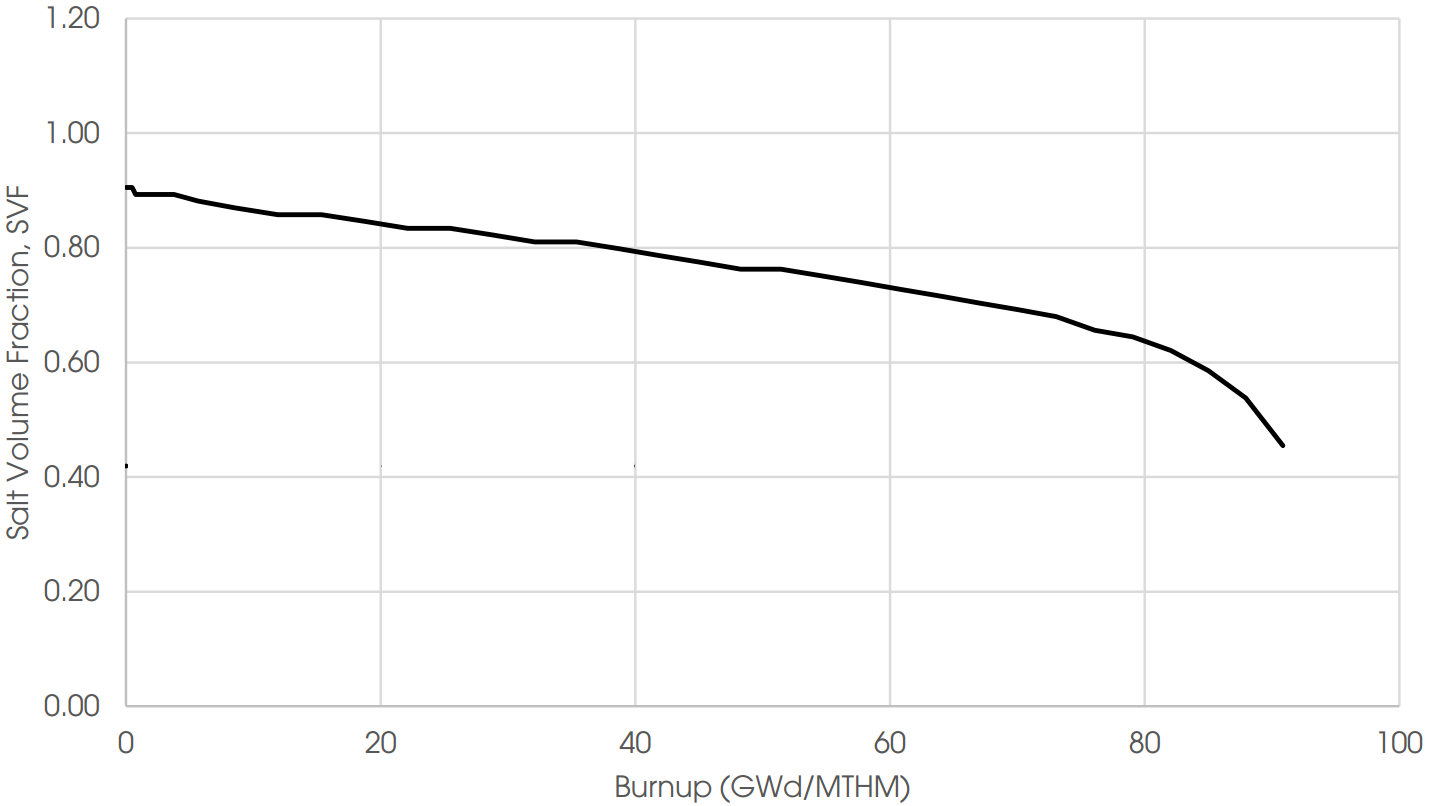
\includegraphics[width=\textwidth]{ch4/svf_predetermined.png}
	\caption{The change in SVF as a function of burnup in the \gls{TAP} 
	reactor (reproduced from Transatomic Power Neutronics Overview  
	\cite{transatomic_power_corporation_neutronics_2016}).}
	\label{fig:svf-predetermined}
\end{figure}


\subsection{Fuel salt reprocessing system}
The \gls{TAP} nuclear system contains a fission product removal system. 
Gaseous \glspl{FP} are continuously removed using an off-gas system while 
liquid and 
solid \glspl{FP} are extracted via a chemical processing system. As these 
byproducts are gradually removed, a small quantity of fresh fuel salt is 
regularly added to the primary loop. This process conserves a constant fuel 
salt mass and keeps the reactor critical. In contrast with the \gls{MSBR} 
reprocessing system, the \gls{TAP} design does not need a protactinium 
separation and isolation system because it operates in a uranium-based 
single-stage fuel cycle. The authors of the \gls{TAP} concept suggested three 
distinct fission product removal methods 
\cite{transatomic_power_corporation_neutronics_2016}:
\paragraph*{Off-Gas System:} The off-gas system removes gaseous fission 
products such as krypton and xenon, which are then compressed and stored 
temporarily until they have decayed to the background radiation level. Trace 
amounts of tritium are also removed and bottled in a liquid form via the same 
process. Also, the off-gas system directly removes a small fraction of the 
noble metals.
\paragraph*{Metal Plate-Out/Filtration:} A nickel mesh filter removes noble 
and semi-noble metal solid fission products as they plate out onto internal 
surface of the filter.
\paragraph*{Liquid Metal Extraction:} Lanthanides and other non-noble metals 
stay dissolved in the fuel salt. They generally have a lower capture cross 
section and thus absorb fewer neutrons than $^{135}$Xe, but their extraction 
is essential to ensure normal operation. In the \gls{TAP} reactor, lanthanide 
removal is accomplished via a liquid-metal/molten salt extraction process 
similar to that developed for \gls{MSBR} by \gls{ORNL}  
\cite{robertson_conceptual_1971}. The process converts the dissolved 
lanthanides into a well-understood oxide waste form, similar to that of 
\gls{LWR} \gls{SNF}. This oxide waste comes out of the \gls{TAP} reprocessing 
plant in ceramic granules and can be sintered into another convenient form for 
storage \cite{transatomic_power_corporation_technical_2016}.

Figure~\ref{fig:tap-reproc} shows the principal design of the \gls{TAP} 
primary loop, including an off-gas system, nickel mesh filter, and lanthanide 
chemical extraction facility. Similarly to the \gls{MSBR}, an off-gas system 
is also based on a simple process of helium sparging through fuel salt with 
consequent gas bubbles removed before returning the fuel salt to the core (see 
Section~\ref{sec:gas-separ}). 
Nevertheless, one crucial difference must be noted: the \gls{MSBR} gas 
separation system suggested helium injection and subsequent transport of the 
voids throughout the primary loop, including the core for at least ten full 
loops \cite{robertson_conceptual_1971}. 
\begin{figure}[htp!] % replace 't' with 'b' to 
	\centering
	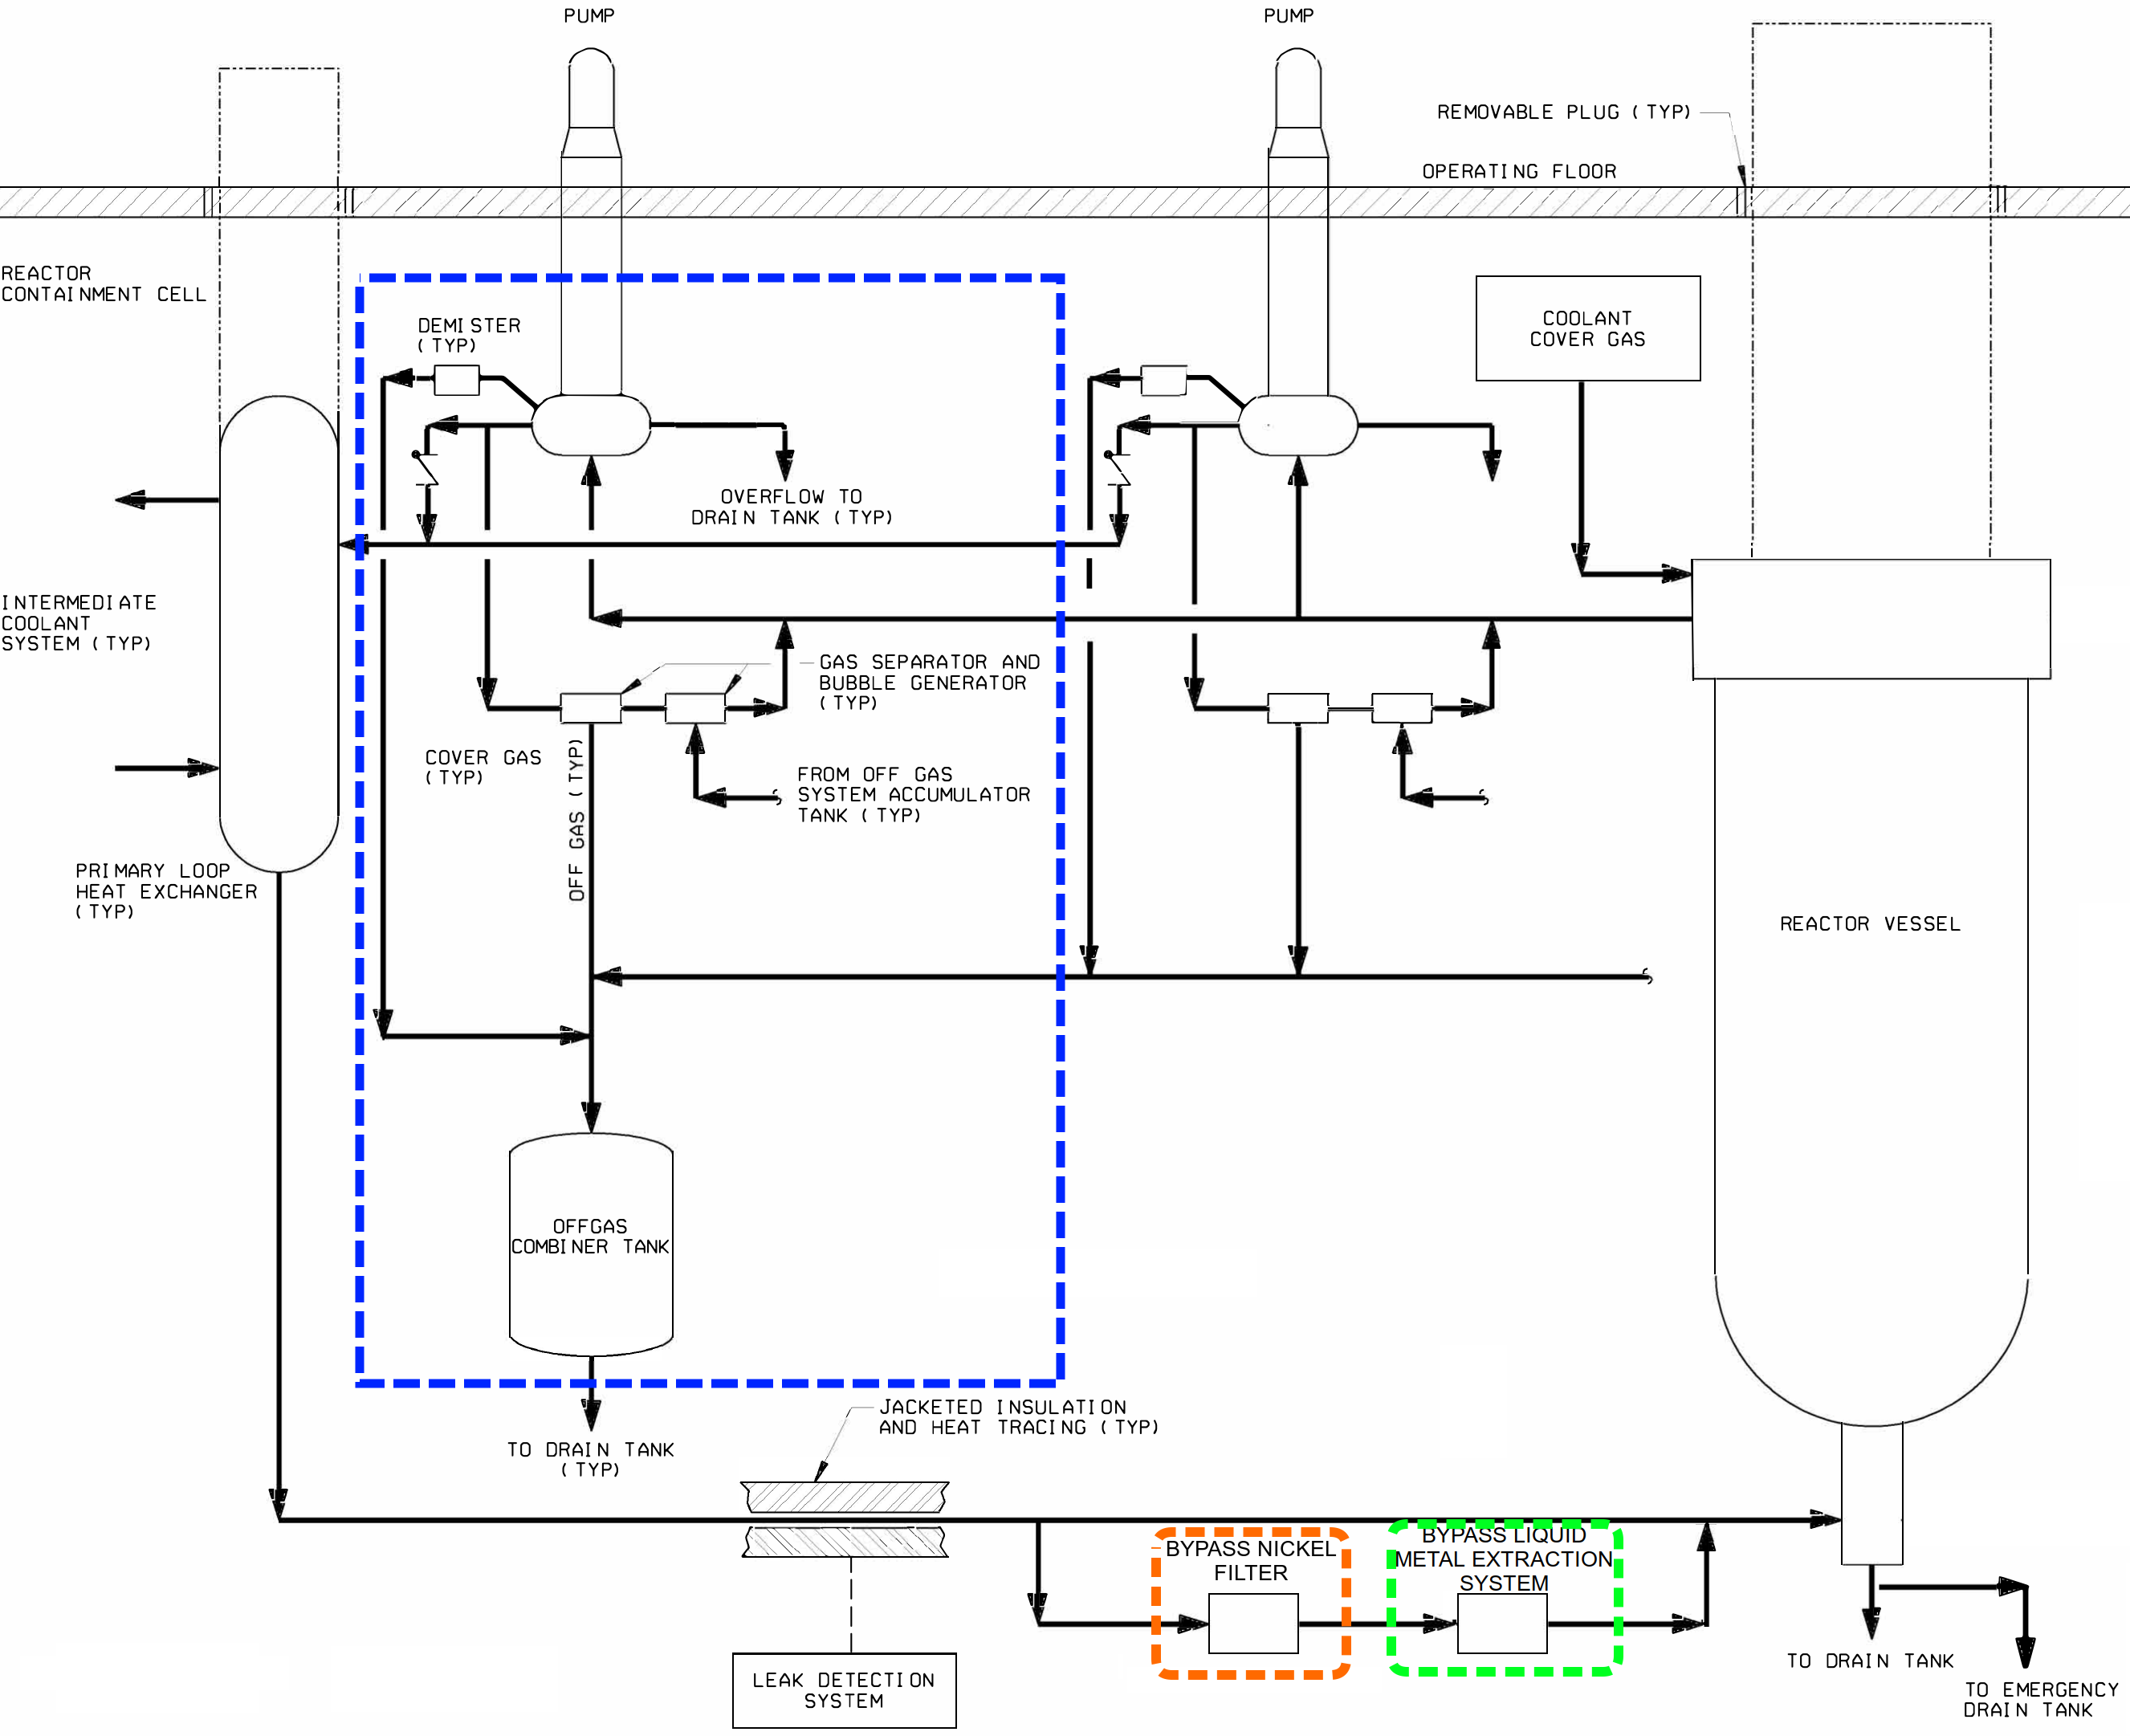
\includegraphics[width=\textwidth]{ch4/tap_primary_loop.png}
	\caption{Simplified \gls{TAP} primary loop design including off-gas system 
		(blue), 
		nickel filter (orange) and liquid metal extraction system (green) 
		(reproduced from \cite{transatomic_power_transatomic_2019}).}
	\label{fig:tap-reproc}
\end{figure}

Introduction of the void (helium bubbles) during operation is a significant 
concern for safe, stable operation because the increase of void fraction in 
the fuel salt when it enters back to the core would cause unpredictable 
reactivity change. Kedl stated, ``Average loop void fractions as high as 1\% 
are undesirable... it is desirable to keep the average loop void fraction well 
below 1\%.''\cite{robertson_conceptual_1971} but he did not offer an 
explanation why. In fact, the \gls{MSBR} design targeted 0.2\% average void in 
the fuel salt \cite{robertson_conceptual_1971} and the \gls{MSRE} successfully 
operated with average void fraction about 0.7\% \cite{compere_fission_1975}.
We can reduce void fraction in the fuel salt to negligible levels by using an 
effective gas separator for stripping helium/xenon bubbles before returning 
the salt to a primary loop (Figure~\ref{fig:tap-reproc}, blue block). 

Noble and semi-noble metal solid fission products tend to plate out onto metal 
surfaces including piping, heat exchanger tubes, reactor vessel inner surface, 
etc. Previous research by \gls{ORNL} \cite{robertson_conceptual_1971} reported 
that about 50\% of noble and semi-noble metals would plate out inside 
\gls{MSBR} systems (including off-gas system) without any special treatment. 
To improve the extraction efficiency of these fission products, the \gls{TAP} 
concept suggested employing a nickel mesh filter located in a bypass stream in 
the primary loop (Figure~\ref{fig:tap-reproc}, orange block). The main idea of 
this filter is to create large nickel surface area using porous metal (e.g., 
Inconel fibers). The fuel salt is flowing throughout the filter and noble 
metals plate-out on the internal filter surface. 

This Liquid Metal Extraction process for the \gls{TAP} concept has been 
adopted from the \gls{MSBR}. The \gls{MSRE} demonstrated a liquid-liquid 
extraction process for removing rare earths and lanthanides from fuel salt and 
estimated efficiency of this process. 
In fact, due to similarities in reprocessing schemes, the \gls{TAP} project 
reported almost the same set of elements for removal and similar effective 
cycle times as suggested for \gls{MSBR} (Table~\ref{tab:reprocessing_list}). 
The \gls{TAP} neutronics whitepaper specifies additional low-probability 
fission products and gases that should be removed during operation. These 
elements are categorized into the previously defined processing groups, but 
the removal rates of most of these elements (all except for hydrogen) 
are very low.

Details of gas removal and fuel reprocessing systems have historically 
been conceptual. Accordingly, liquid-fueled system design including the 
\gls{TAP} concept usually assumes ideal (rather than realistically 
constrained) removal efficiencies for reactor performance simulations. In this 
thesis, I developed a realistic online reprocessing system and reactor model 
to capture the dynamics of fuel composition evolution during reactor 
operation. Gas removal efficiency is variable in that model, described using 
mathematical correlation from Chapter 2 (see Equation~\ref{eq:gas_eff}). For 
the other \glspl{FP}, a fixed\footnote{Published information about dynamics of 
extraction efficiency during reactor operation for noble-, seminoble metals, 
and rare earths is insufficient to inform a variable removal efficiency.}, 
non-ideal extraction efficiency based on cycle time from  
Table~\ref{tab:reprocessing_list} was used to inform the fuel reprocessing 
model.

%%%%%%%%%%%%%%%%%%%%%%%%%%%%%%%%%%%%%%%%
\begin{table}[htp!]
	\centering
	\caption{The effective cycle times for fission products removal  from the 
		\gls{TAP} reactor (reproduced from \cite{betzler_implementation_2017} 
		and 
		\cite{transatomic_power_corporation_neutronics_2016}).}
	\begin{tabular}{p{0.2\textwidth} p{0.42\textwidth} p{0.12\textwidth} 
			p{0.14\textwidth}}
		\hline 
		%\begin{tabularx}{\linewidth}{l X} \toprule 
		\textbf{Processing group} & \qquad\qquad\qquad \textbf{Nuclides} & 
		\textbf{Removal Rate (s$^{-1}$)} & \textbf{Cycle time (at full power)} 
		\\ [5pt] \hline 
		\multicolumn{3}{c}{\textit{Elements removed in the \gls{MSBR} concept 
		and adopted for the \gls{TAP}} \cite{robertson_conceptual_1971}} \\
		Volatile gases & Xe, Kr								  & 5.00E-2 & 20 
		sec \\ [5pt]
		Noble metals & Se, Nb, Mo, Tc, Ru, Rh, Pd, Ag, Sb, Te & 5.00E-2 & 20 
		sec \\ [5pt]
		Seminoble metals & Zr, Cd, In, Sn	  				  & 5.79E-8 & 200 
		days \\ [5pt]
		Volatile fluorides & Br, I 							  & 1.93E-7 & 60 
		days \\ [5pt]
		Rare earths & Y, La, Ce, Pr, Nd, Pm, Sm, Gd           & 2.31E-7 & 50 
		days \\ [5pt]
		\qquad & Eu & 2.32E-8 & 500 days \\ [5pt]
		Discard & Rb, Sr, Cs, Ba & 3.37E-9 & 3435 days \\ [5pt] 
		\hline
		
		\multicolumn{3}{c}{\textit{Additional elements removed} 
			\cite{transatomic_power_corporation_neutronics_2016, 
				betzler_implementation_2017}  } \\
		Volatile gases & H								  	& 5.00E-2 & 20 
		sec    \\ [5pt]
		Noble metals & Ti, V, Cr, Cu						& 3.37E-9 & 3435 
		days \\ [5pt]
		Seminoble metals & Mn, Fe, Co, Ni, Zn, Ga, Ge, As   & 3.37E-9 & 3435 
		days \\ [5pt]
		Rare earths & Sc									& 3.37E-9 & 3435 
		days \\ [5pt]
		Discard & Ca										& 3.37E-9 & 3435 
		days \\ [5pt] 
		\hline
	\end{tabular}
	\label{tab:reprocessing_list}
	\vspace{-0.9em}
\end{table}
%%%%%%%%%%%%%%%%%%%%%%%%%%%%%%%%%%%%%%%%%%%%%%%%%%%%%%%%%%%%%%%%%%%%%%%%%%%%%%%


\section{TAP system model} \label{sec:tap_model}
In this section, the \gls{TAP} core and fuel salt reprocessing system models  
for demonstrating SaltProc v1.0 are described in details. I used these models 
for SaltProc demonstration and validation for both long-term and short-term 
cases.

\subsection{Serpent 2 full-core model} 
Nest and lattice geometry types as well as universe transformation 
capabilities of Serpent \cite{leppanen_serpent_2014} are employed to 
represent \gls{TAP} core. Figure~\ref{fig:tap-serpent-plan} shows $XY$ section 
of the whole-core model at the expected reactor operational level 
when all control rods are fully withdrawn. Figures~\ref{fig:tap-serpent-elev} 
and \ref{fig:tap-serpent-elev-zoom} show a longitudinal section of the 
reactor. This model contains the moderator rods with silicon carbide cladding, 
pressure vessel, and inlet and outlet plena (Table~\ref{tab:tap_model_param}). 
Fuel salt flows around square moderator assemblies consisting of lattices 
of small-diameter zirconium hydride rods in a corrosion-resistant material. 
The salt volume fraction for Figure~\ref{fig:tap-serpent-plan} is 0.917204, 
which means the modeled core is under-moderated and has intermediate neutron 
spectrum. Quarter-core configurations of the \gls{TAP} core with various salt 
volume fraction, used in the current work to maintain criticality for 
reasonable operational period ($>20$ years), are listed in 
Table~\ref{tab:tap_adjustable_core}, Figures~\ref{fig:tap-406-681}, and 
\ref{fig:tap-840-1668} in Appendix~\ref{appex:geometries}.
\begin{figure}[htp!] % replace 't' with 'b' to 
	\centering
	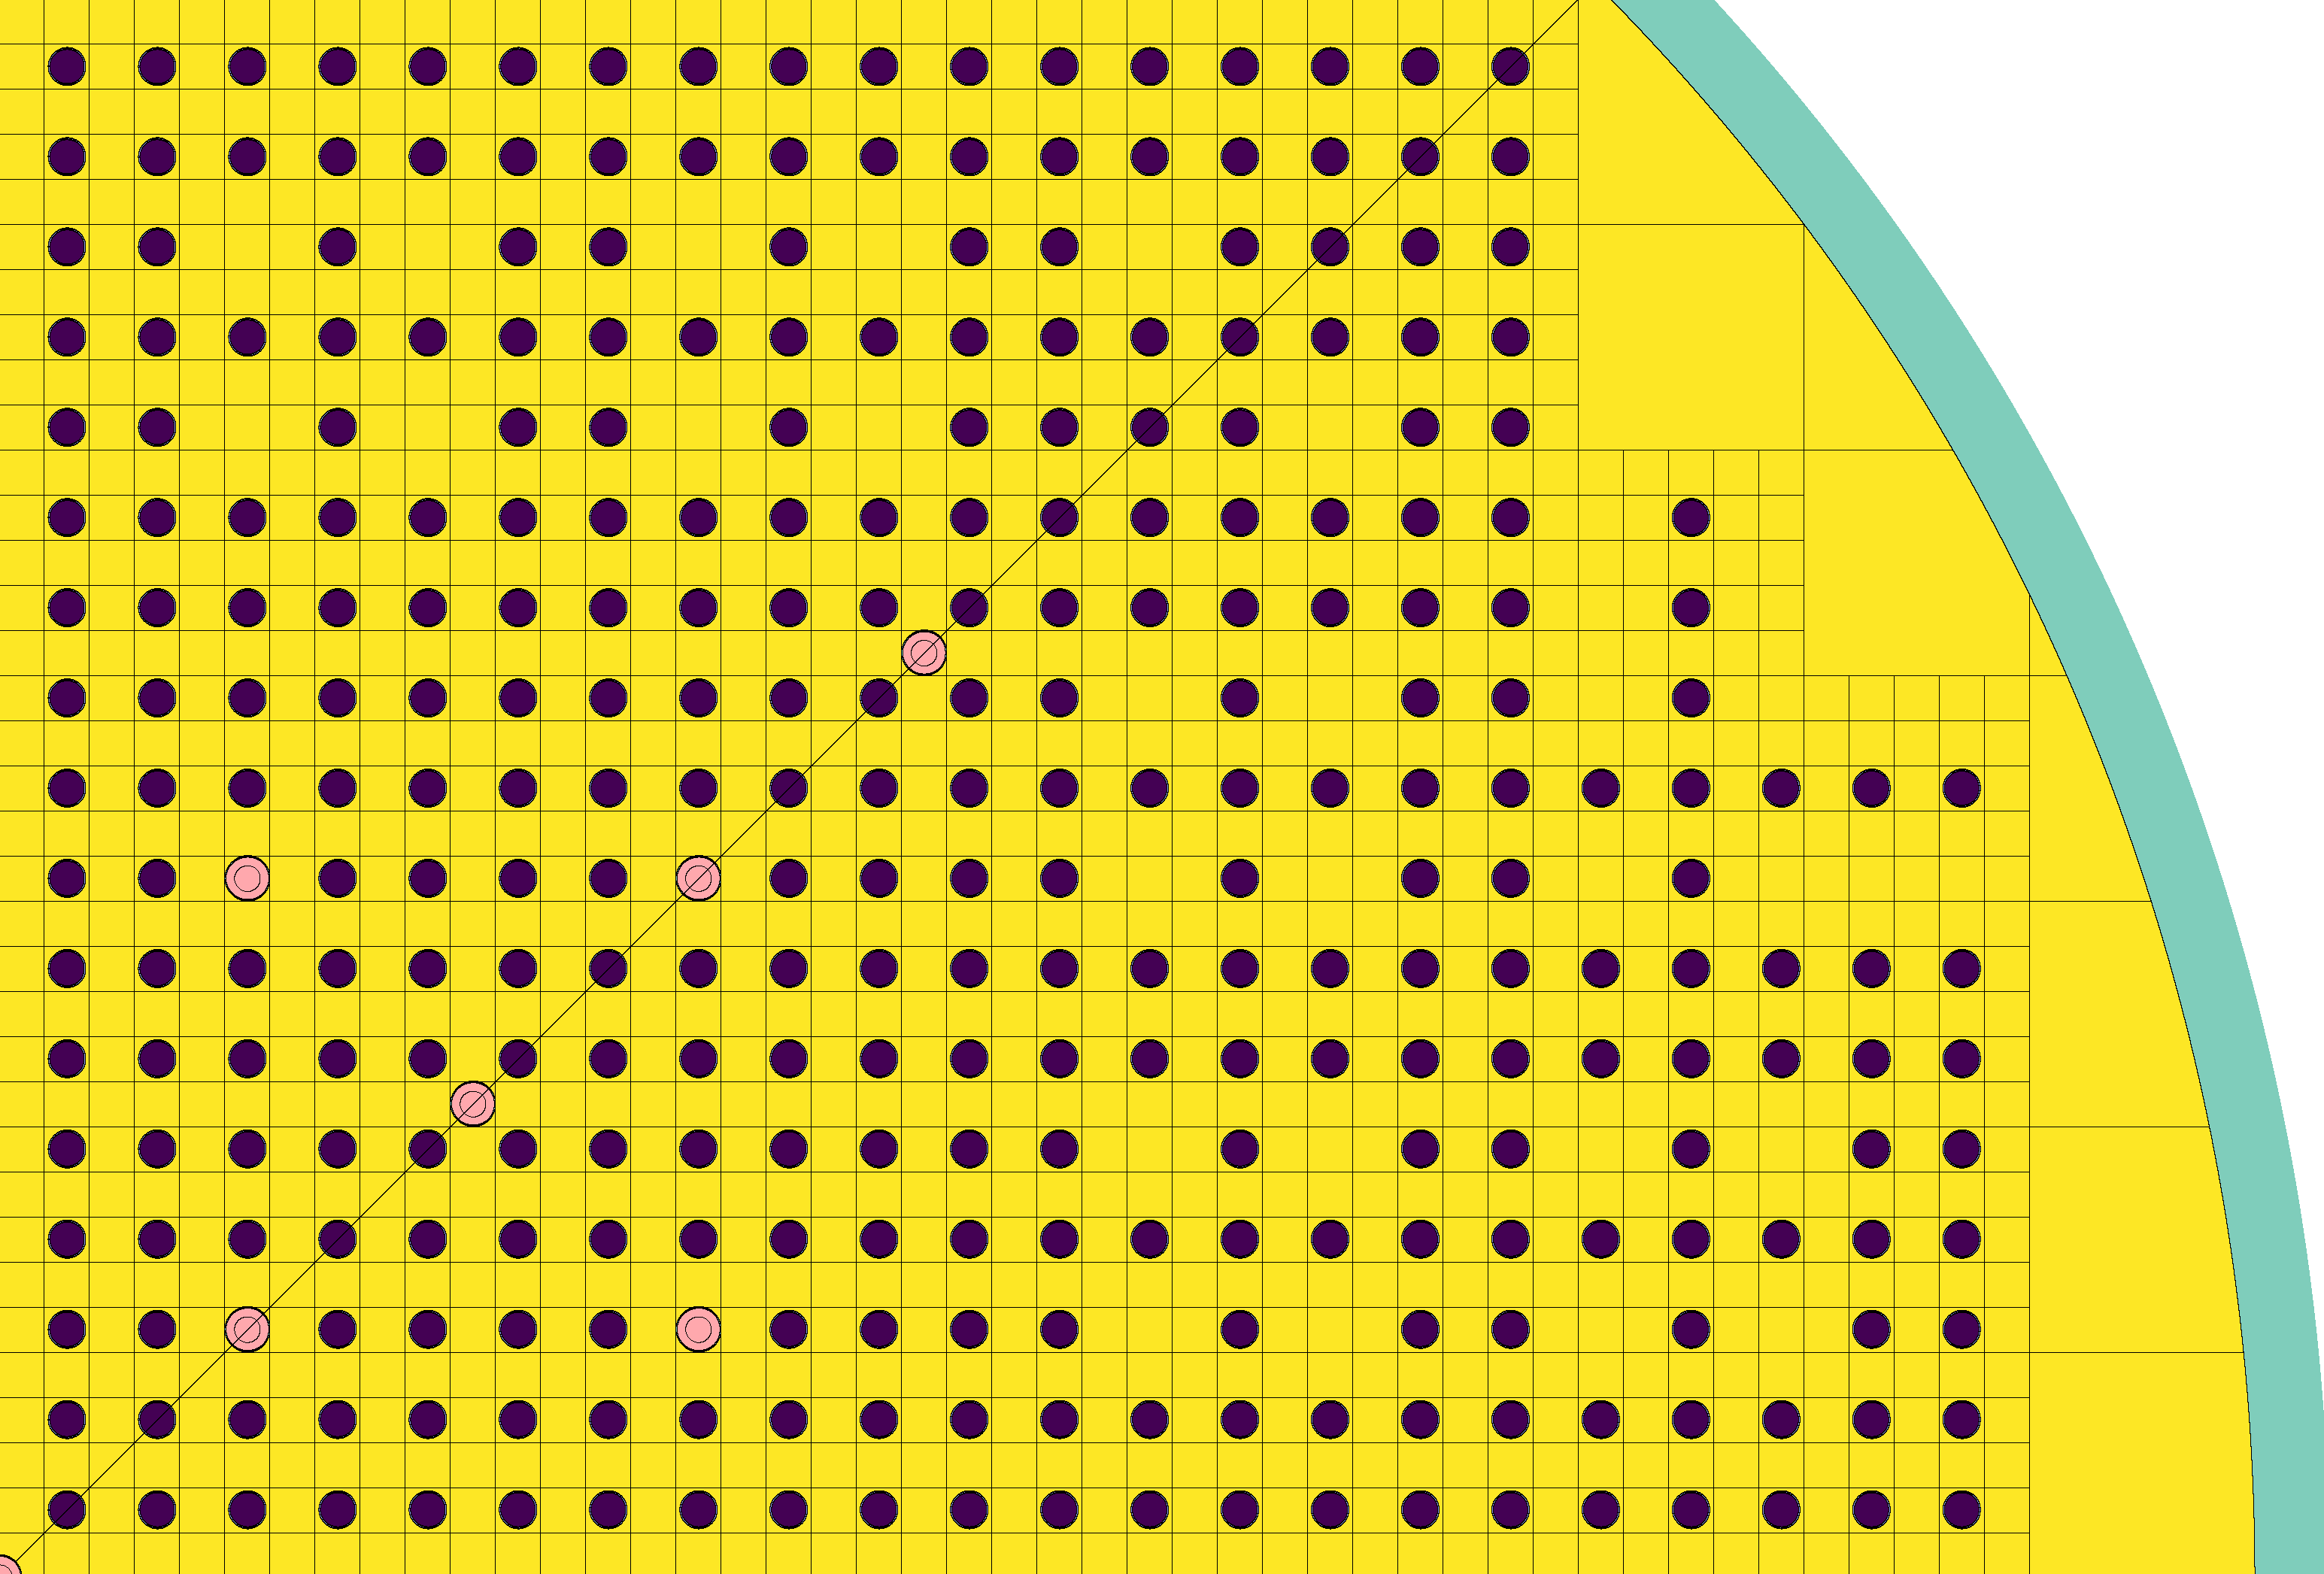
\includegraphics[width=0.75\textwidth]{ch4/tap_plan_view_serpent_347.png}
	\caption{An $XY$ section of the \gls{TAP} model at horizontal midplane 
		with fully withdrawn control rods at \gls{BOL} (347 moderator rods, 
		salt volume fraction 0.917204). 
		The violet color represents zirconium hydride, and the yellow 
		represents fuel salt. 
		The blue color shows Hastelloy-N, a material used for the vessel wall, 
		and the pink color is the air.}
	\label{fig:tap-serpent-plan}
\end{figure}

\begin{figure}[htp!] % replace 't' with 'b' to 
	\centering
	
\includegraphics[width=0.6\textwidth]{ch4/tap_elev_view_serpent_347.png}
	\caption{45$^{\circ}$ $XZ$ section of the \gls{TAP} core model.}
	\label{fig:tap-serpent-elev}
\end{figure}

To represent the reactivity control system, the model has: 
\begin{enumerate}[label=(\alph*), noitemsep]
	\item control rod guide tubes made of nickel-based alloy;
	\item control rods represented as a Boron Carbide (B$_4$C) cylinders 
	with a thin Hastelloy-N coating;
	\item air inside guide tubes and control rods;
\end{enumerate}
The control rods must be able to suppress excess reactivity at the \gls{BOL} 
when the core configuration is the most reactive and the neutron spectrum is 
the hardest. The control rod design shown on 
Figures~\ref{fig:tap-serpent-plan}, \ref{fig:tap-serpent-elev} and 
\ref{fig:tap-serpent-elev-zoom} is 
comprised of a cluster of 25 rods that provide a total reactivity worth of 
$4226\pm9pcm$ at the \gls{BOL}.

\begin{figure}[hbp!] % replace 't' with 'b' to 
	\centering
	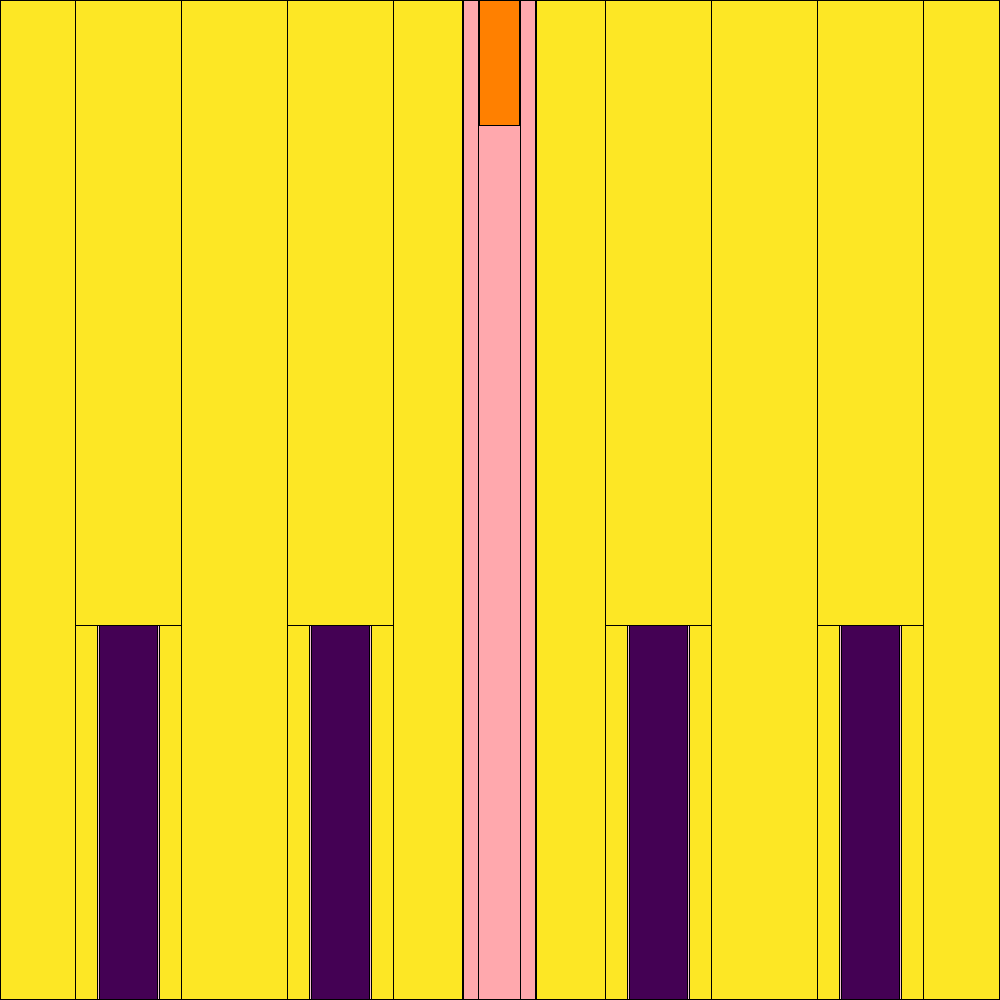
\includegraphics[width=0.55\textwidth]{ch4/tap_elev_view_zoomed_serpent.png}
	\caption{Zoomed $XZ$ section of the top of the moderator and control rods  
		in the \gls{TAP} model. The orange color shows Boron Carbide 
		(B$_4$C) absorbers used for control rods.}
	\label{fig:tap-serpent-elev-zoom}
\end{figure}
%%%%%%%%%%%%%%%%%%%%%%%%%%%%%%%%%%%%%%%%%%%%%%%%%%
\begin{table}[ht!]
	\caption{Geometric parameters for the full-core 3D model of the 
		\gls{TAP} (reproduced from Betzler \emph{et al.} 
		\cite{betzler_assessment_2017-1}). }
	\centering
	\begin{tabularx}{0.9\textwidth}{s s x p{0.14\textwidth}}
		\hline
		\textbf{Component}&\textbf{Parameter}&\textbf{Value}& \textbf{Unit}   
		\\ \hline
		\multirow{4}{*}{\begin{tabular}[c]{@{}l@{}}Moderator\\ 
				rod\end{tabular}} 
		& Cladding thickness      	  			    & 0.10 & cm				 
		\\  
		& Radius 				      	  			& 1.15 & cm				 
		\\  
		& Length				      	  			& 3.0  & m				 
		\\  
		& Pitch				      	  			& 3.0  & cm  			 \\ 
		\hline 
		
		\multirow{2}{*}{\begin{tabular}[c]{@{}l@{}}Moderator\\ 
				assembly\end{tabular}} 
		& Array				      	  			& 5 $\times$ 5 & 
		rods$\times$rods \\  
		& Pitch				      	  			& 15.0 & cm    				 
		\\  \hline
		
		\multirow{4}{*}{\begin{tabular}[c]{@{}l@{}}Core\end{tabular}}          
		& Assemblies  				   	  			& 268  & assemblies/core 
		\\  
		& Inner radius			      	  			& 1.5  & 
		m    				 \\  
		& Plenum height			   	  			& 25.0 & cm    				 
		\\  
		& Vessel wall thickness     	  			& 5.0 & 
		cm    				 \\ \hline            
	\end{tabularx}
	\label{tab:tap_model_param}
\end{table}
%%%%%%%%%%%%%%%%%%%%%%%%%%%%%%%%%%%%%%%%%%%%%%%%

The control rod cluster is modeled using the \textbf{TRANS} Serpent 2 feature, 
which allows the user to easily change the control rod position during the 
simulation. The current works assumed that all control rods are fully 
withdrawn from the core (Figure~\ref{fig:tap-serpent-elev-zoom}), but user can 
use SaltProc v1.0 reactivity control capabilities to change control 
rod position during operation. In this dissertation, all figures of the core 
were generated using the built-in Serpent plotter.

The neutron population per cycle and the number of active/inactive cycles were 
chosen to obtain a balance between minimizing uncertainty for a transport 
problem (28 pcm for $k_{eff}$) and simultaneously minimizing computational 
time.


\subsection{Model of the fuel reprocessing system}
I thoroughly analyzed the original \gls{TAP} reprocessing system design 
(Figure~\ref{fig:tap-reproc}) and neutron poisons removal rates  
(Table~\ref{tab:reprocessing_list}) to determine a suitable reprocessing 
scheme for SaltProc v1.0 demonstration (Figure~\ref{fig:demo-repro-scheme}). 
This chapter presents two demonstration cases: with ideal 
(Section~\ref{sec:ben-valid}) and realistic, non-ideal 
(Section~\ref{sec:long-term-real}) gas removal efficiency. Realistic noble gas 
removal efficiency is based on physical model for noble gas extraction 
efficiency discussed in Section~\ref{sec:gas-separ}. 
\begin{figure}[htp!] % replace 't' with 'b' to 
	\centering
	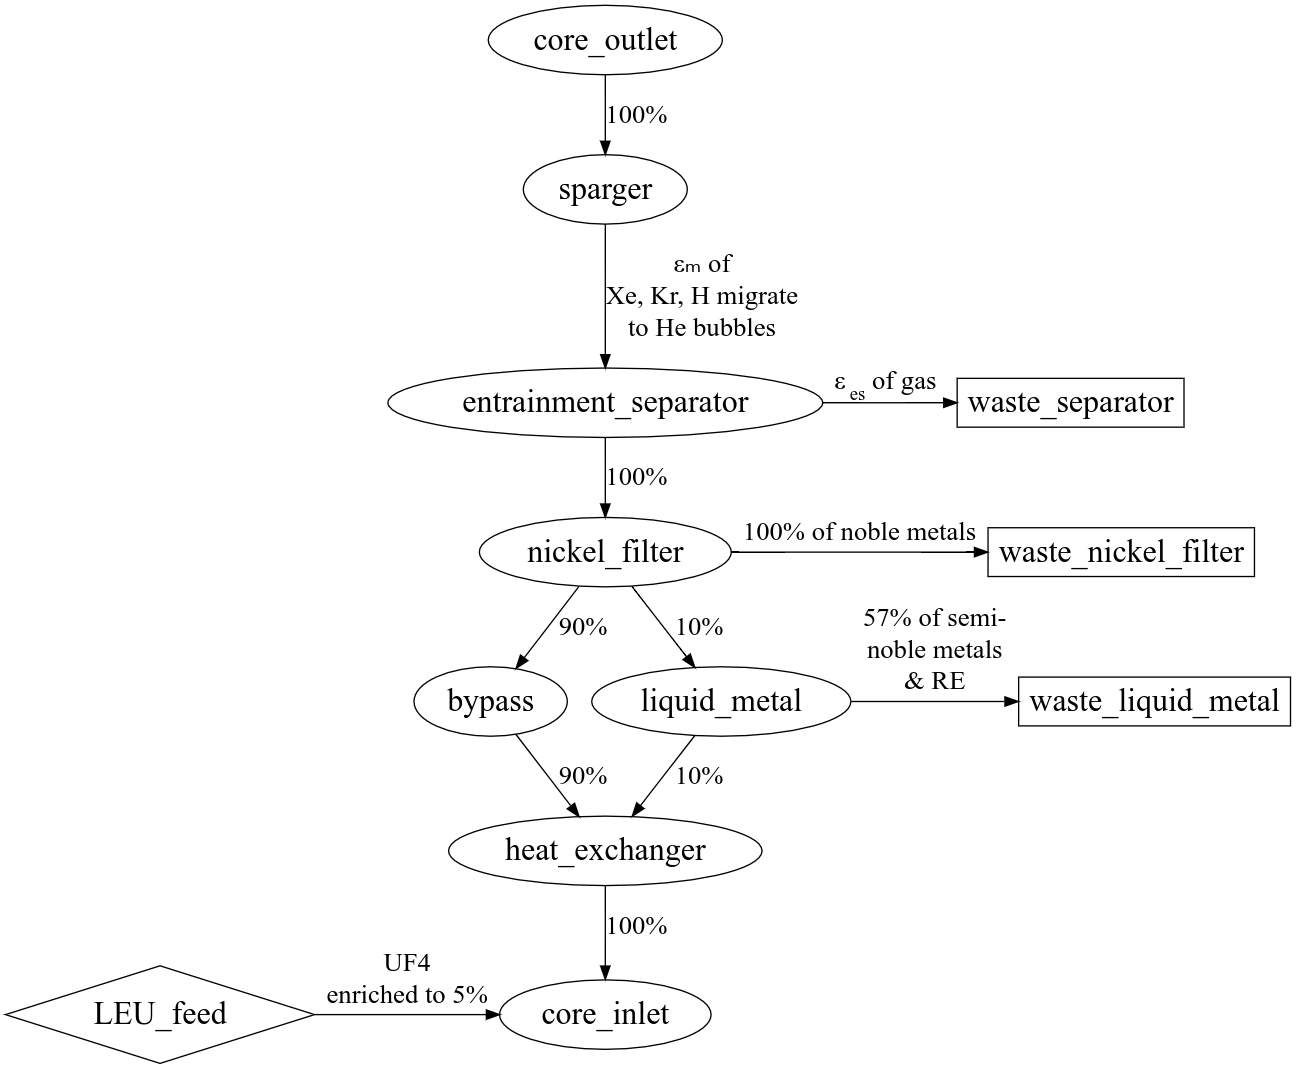
\includegraphics[width=\textwidth]{ch4/tap_saltproc_var_eps.png}
	\caption{\gls{TAP} reprocessing scheme flowchart used for demonstration of 
	SaltProc v1.0. Arrows represent material flow; percents represent fraction 
	of total mass flow rates; ellipses represent fuel reprocessing system 
	components; boxes represent waste streams; the diamond shows refuel 
	material flow (UF$_4$, 5 wt\% of $^{235}$U). Efficiency of gas migration 
	to 	helium bubbles 	($\epsilon_m$) and efficiency of gas bubbles 
	separation from the salt ($\epsilon_{es}$) are different for various 
	demonstration cases and discussed in more detail in 
	Sections~\ref{sec:ben-valid} and \ref{sec:long-term-real}. Efficiency of 
	noble metals extraction in the nickel filter 
	(Figure~\ref{fig:tap-primary-scheme}, orange block) and 	
	seminoble metals/rare earths (RE) in the liquid metal extraction system 
	(Figure~\ref{fig:tap-primary-scheme}, green block) is assumed fixed 	
	and equal 100\% and 57\%, respectively.}
	\label{fig:demo-repro-scheme}
\end{figure}

The gas removal components (sparger/contactor and entrainment separator) are 
located in-line because estimated full loop time for the fuel salt is about 20 
seconds and approximately equal to the cycle time 
(Table~\ref{tab:reprocessing_list}). To extract volatile gases every 20 
seconds, the gas removal system must operate with 100\% of the core throughout 
flow rate (in-line gas removal system). In this chapter, efficiency of noble 
gas migration to helium bubbles and efficiency of bubbles removal from the 
salt by entrainment separator ($\epsilon_m,\epsilon_{es}$ on  
Figure~\ref{fig:demo-repro-scheme}, respectively) are selected separately for 
each demonstration case.

The nickel filter in the \gls{TAP} concept is designed to extract 
noble/semi-noble metals and volatile fluorides 
(Table~\ref{tab:reprocessing_list}). Similarly to volatile gases, 
noble metals must be removed every 20 seconds and, hence, the filter should 
operate with 100\% of the core throughout flow rate. The nickel filter removes 
a wide range of elements with various effective cycle time 
(Table~\ref{tab:reprocessing_list}).

Lanthanides and other non-noble metals generally have a lower capture  
cross section and absorb fewer neutrons than gases and noble metals. These 
elements can be removed via a liquid-metal/molten salt extraction process with 
relatively low removal rates (cycle time $> 50$ days). This is accomplished 
by directing a small fraction of the salt mass flow leaving the nickel mesh 
filter (10\% of the core throughout flow rate) to the liquid-metal/molten salt 
component of the reprocessing system, where lanthanides are removed with a 
specific extraction efficiency to match the  required cycle time 
(Table~\ref{tab:reprocessing_list}). The rest 90\% of the salt mass flow is 
directed from the nickel filter to heat exchanger without performing any fuel 
salt treatment.

The removal rates vary among nuclides in this reactor concept, which dictate 
the necessary resolution of depletion calculations. To compromise, a 3-day 
depletion time step was selected for the long-term demonstration case based on 
a time step refinement study by Betzler \emph{et al.} 
\cite{betzler_assessment_2017-1}. Complimentary time step refinement study 
results are presented in Section~\ref{sec:time-refinement}.

\section{Long-term depletion demonstration and validation}
\subsection{Constant, ideal extraction efficiency case}\label{sec:ben-valid}
To validate SaltProc v1.0, I performed lifetime-long depletion calculation 
with ideal extraction efficiency. This case was selected to repeat fuel salt 
depletion as close as possible to ChemTriton simulation for full-core 
\gls{TAP} core by Betzler \emph{et al.} \cite{betzler_assessment_2017-1}.  
Betzler \emph{et al.} made following assumptions and approximations in their 
work \cite{betzler_assessment_2017-1}:
\begin{enumerate}[noitemsep]	
	\item Effective cycle times as prescribed by Transatomic Power Technical 
	White Paper (Table~\ref{tab:reprocessing_list}) with \textbf{100\% noble 
	gas removal efficiency}; hence, $\epsilon_{es}$ and $\epsilon_m$ in 
	reprocessing model (Figure~\ref{fig:demo-repro-scheme}) are both set to 
	1.0.
	\item 5\% \gls{LEU} feed rate is equal to rate of fisson product removal.
	\item 3-day depletion step.
	\item Quarter-core, 3-D model with vacuum boundary conditions.
	\item Delayed neutron precursor drift was neglected.
\end{enumerate}
I adopted those assumption for code-to-code verification of SaltProc v1.0 
against ChemTriton. ENDF/B-VII.1 \cite{chadwick_endf/b-vii.1_2011} nuclear 
data library is used for this case to be consistent with Betzler's work.
Unfortunately, some crucial details has not been reported in 
\cite{betzler_assessment_2017-1}: (1) exact core geometries for various 
moderator rod configurations except startup configuration; (2) excess 
reactivity at startup; (3) library from which S($\alpha, \beta$) tables for 
thermal scattering in zirconium hydride are obtained. This section presented 
my best effort to repeat Betzler \emph{et al.} simulation using same input 
data to validate SaltProc for the \gls{TAP} concept.


\subsubsection{Effective multiplication factor dynamics}
Figures~\ref{fig:keff-ben-valid} and \ref{fig:keff-ben-valid-zoomed} 
demonstrate the effective multiplication factor obtained using SaltProc v1.0 
with Serpent. The $k_{eff}$ was obtained after removing fission products and 
adding feed material at the end of each depletion step (3 days for this case). 
SaltProc v1.0 updated the moderator rod configuration to the next 
configuration (e.g., from 1388 rods per core to 1624 rods per core) once 
predicted value of $k_{eff}$ at the end of next depletion step drops below 1. 
This algorithm mimics regular maintenance shutdown when the \gls{TAP} core 
excess reactivity is exhausted, and moderator rod assemblies should be 
reconfigured to operate next cycle. 

Optimal number of moderator configurations (cycles) is found to be 15 (see 
Appendix~\ref{appex:geometries}). Fewer cycles would improve capacity factor 
but needs larger excess reactivity at the \gls{BOC} which is strictly limited 
by reactivity control system worth. More cycles would require frequent 
moderator rods reconfiguration which worsen capacity factor.  The interval 
between first and second moderator configuration was only 12 months, the 
shortest interval between moderator configuration updates. For the operation 
interval between 2 and 16 years after startup, the intervals between shutdowns 
for moderator rod updates was 18-26 months. But towards the \gls{EOL}, the 
intervals between moderator rod reconfiguration dropped to 13 months. Overall, 
average interval between regular shutdowns for the core reconfiguration was 18 
months which exactly matches refueling interval for conventional \glspl{LWR}  
and consistent with Betzler \emph{et al.} ($\approx$16 months)  
\cite{betzler_assessment_2017-1}.
\begin{figure}[htp!] % replace 't' with 'b' to 
	\centering
	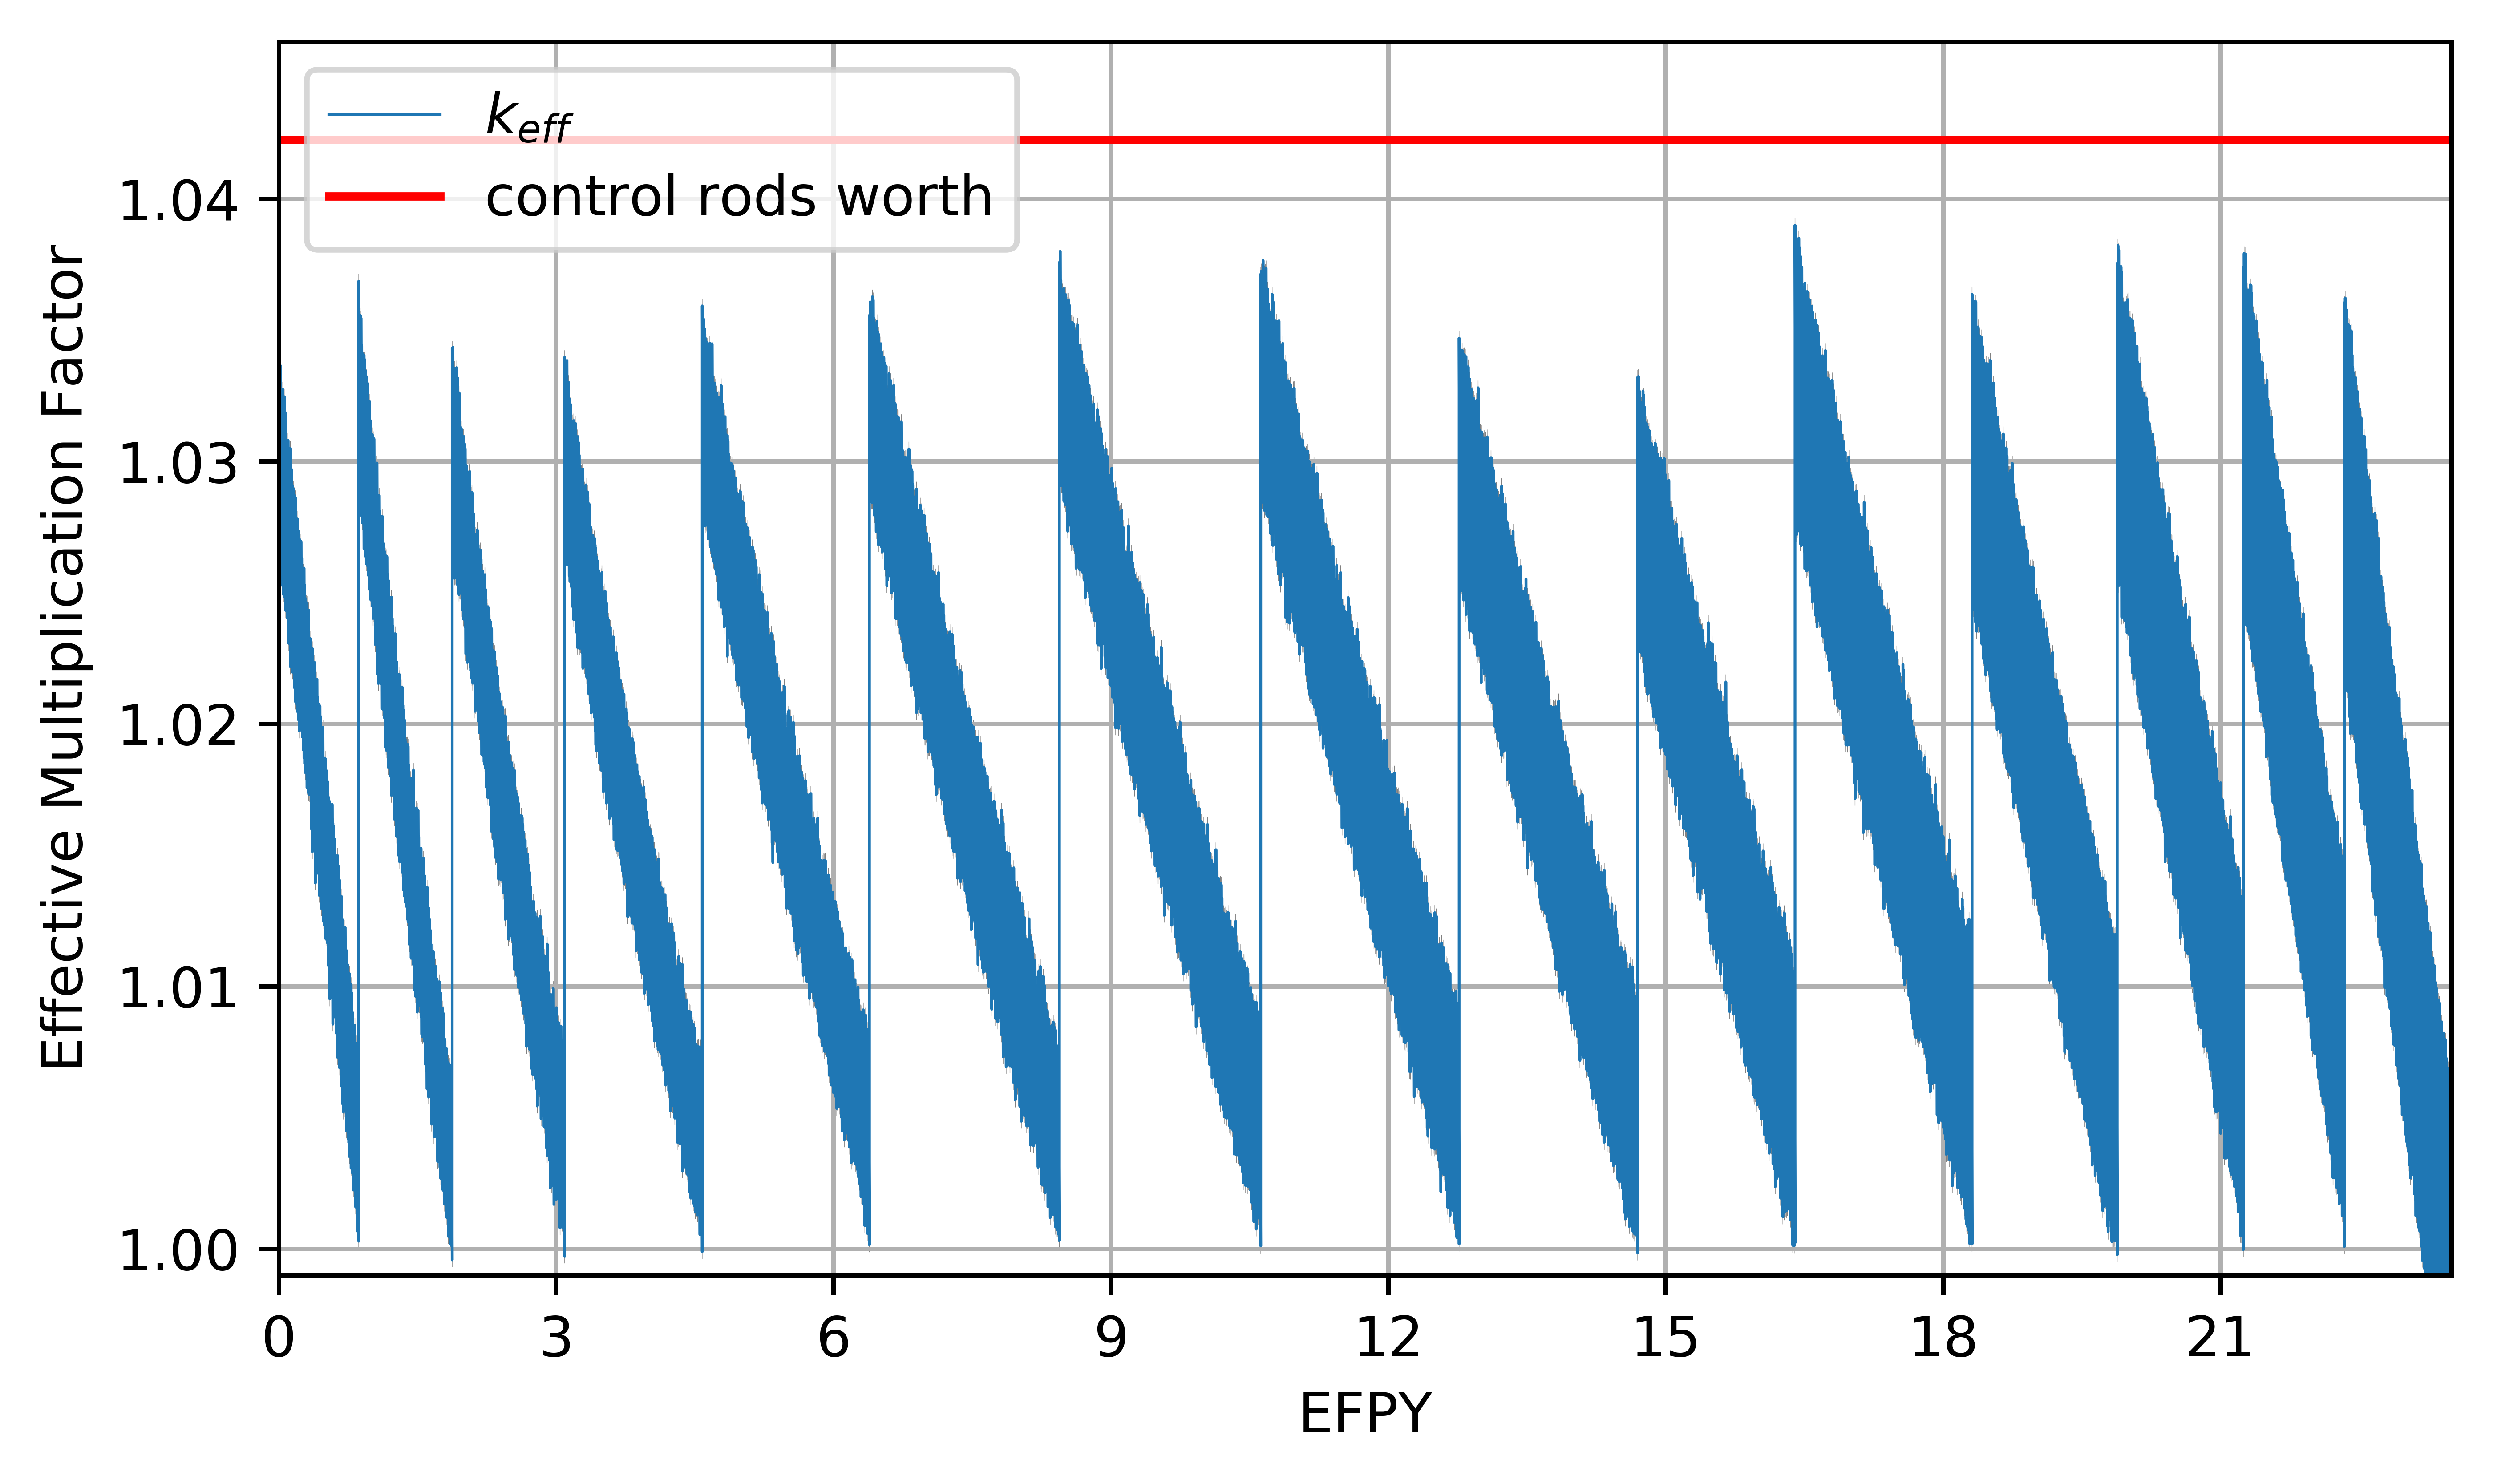
\includegraphics[width=\textwidth]{ch4/keff_ben.png}
	\caption{Effective multiplication factor dynamics during 23.5 years of 
	operation for full-core \gls{TAP} core model for the case with ideal 
	removal efficiency of fission product. Confidence interval $\sigma=28$ 
	$pcm$ is shaded.}
	\label{fig:keff-ben-valid}
\end{figure}

The $k_{eff}$ fluctuates significantly as a result of the batch-wise nature of 
the online reprocessing approach used. Loading the initial fuel salt 
composition with 5\% \gls{LEU} into the \gls{TAP} core leads to a 
supercritical configuration with an excess reactivity of about 3200pcm 
(Figure~\ref{fig:keff-ben-valid}). Without performing any fuel salt 
reprocessing and spectrum shifting, the core became subcritical after 30 days 
of operation \cite{rykhlevskii_milestone_2019}. SaltProc calculates an 
operational lifetime of 22.5 years, after which the fuel salt reached a total 
burnup of 81.46 MWd/kgU. The end of operational lifetime is achieved when the 
minimum \gls{SVF} is obtained, as restricted by the moderator geometry 
parameters (e.g., moderator rod diameter, rod pitch, internal diameter of the 
reactor vessel). Table~\ref{tab:valid_ben_lifetime} compares obtained 
results with Betzler \emph{et al.} \cite{betzler_assessment_2017-1}. Overall, 
SaltProc-calculated operational lifetime and burnup are lower than the 
reference by approximately 22\% and 17\%, respectively. Better match in the 
operational lifetime between SaltProc v1.0 and ChemTriton can be obtained if 
detailed moderator configuration description of Betzler \emph{et al.} model 
will be available in a future.
\begin{figure}[htp!] % replace 't' with 'b' to 
	\centering
	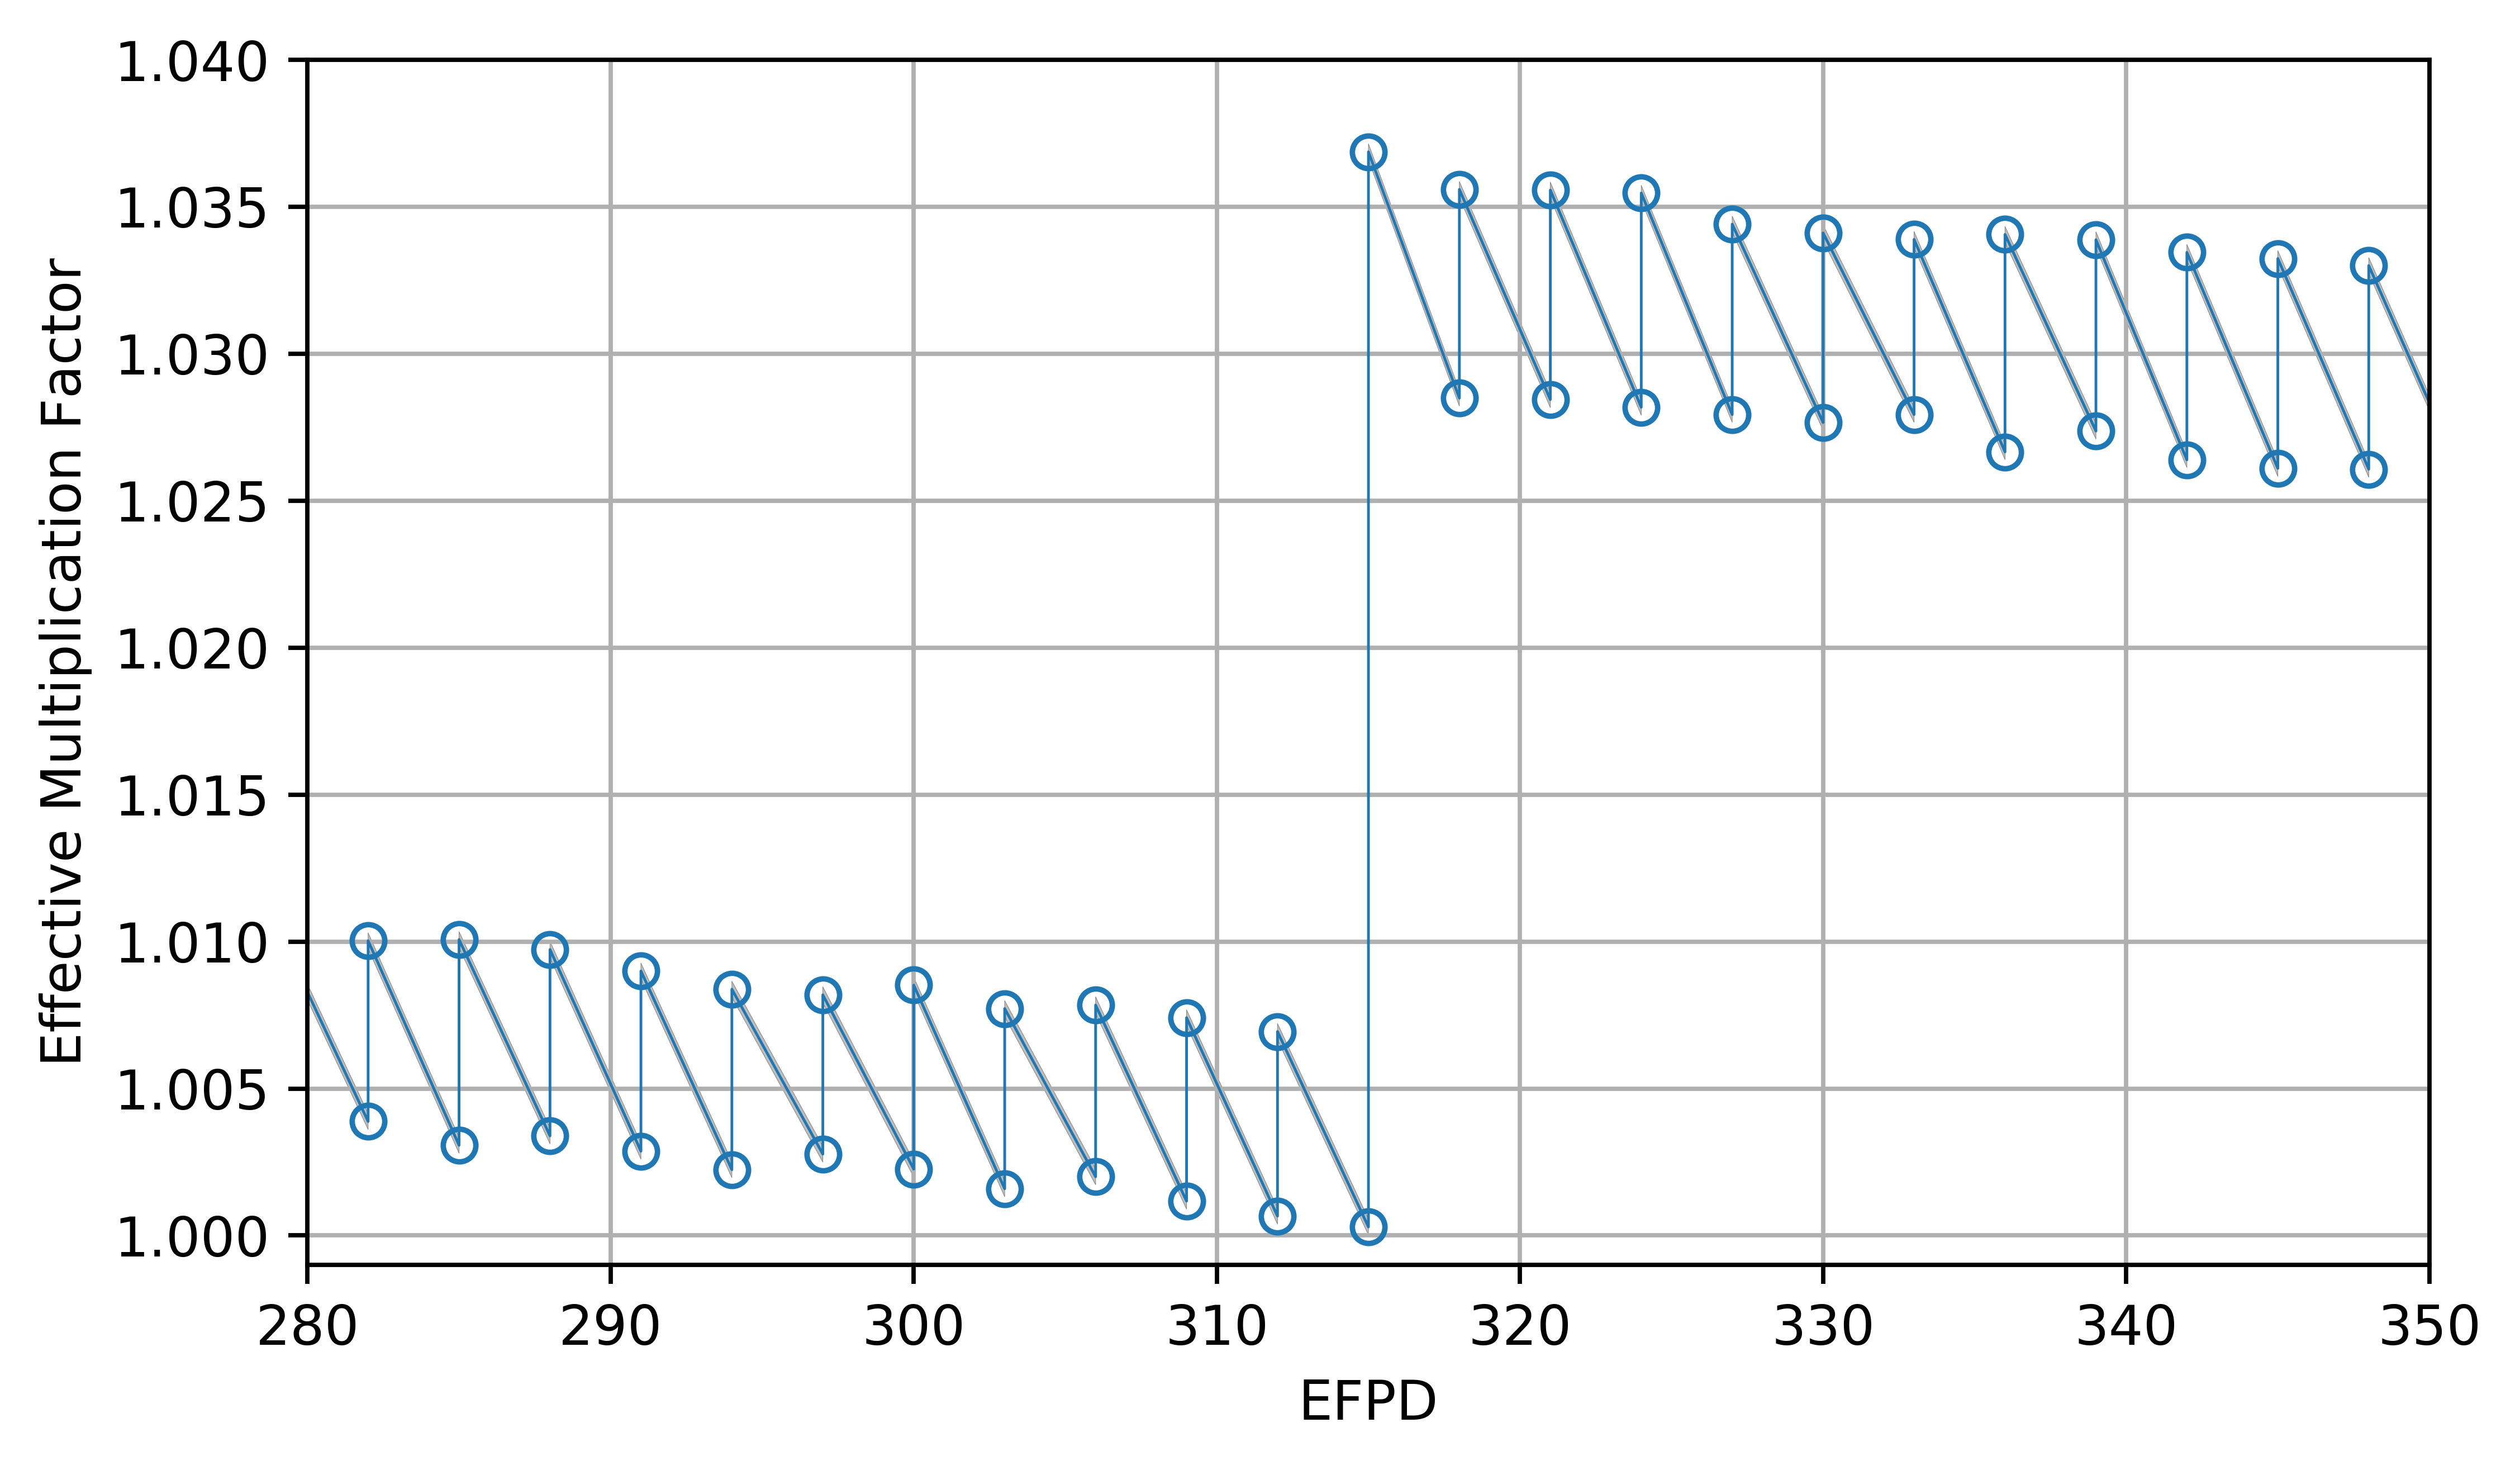
\includegraphics[width=0.9\textwidth]{ch4/keff_ben_zoomed.png}
	\caption{Zoomed effective multiplication factor for the interval from 280 
		to 350 EFPD during transitioning from Cycle \#1 (startup geometry 
		configuration, 347 moderator rods, \gls{SVF}=0.91720353) to Cycle \#2 
		(\gls{SVF}=0.88694). Confidence interval $\sigma=28$ $pcm$ is 
		shaded.}
	\label{fig:keff-ben-valid-zoomed}
\end{figure}
%%%%%%%%%%%%%%%%%%%%%%%%%%%%%%%%%%%%%%%%
\begin{table}[htp!]
	\centering
	\caption{Comparison of main operational parameters in the \gls{TAP} 
	reactor between the current work and Betzler \emph{et al.}
	\cite{betzler_assessment_2017-1}.}
	\begin{tabularx}{\textwidth}{p{0.42\textwidth} R R}
		\hline
		\textbf{Parameter}  & \textbf{Current work} & \textbf{Betzler, 2017} 
		\cite{betzler_assessment_2017-1}\\ \hline
		Operational lifetime [y] & 22.5 & 29.0 \\
		Discharge burnup [MWd/kgU] & 76.30& 91.9 \\
		Average interval between moderator reconfiguration [months] & 18 & 
		16 \\
		\hline
	\end{tabularx}
	\label{tab:valid_ben_lifetime}
\end{table}
%%%%%%%%%%%%%%%%%%%%%%%%%%%%%%%%%%%%%%%%%%%%%%%%%%%%%%%%%%%%%%%%%%%%%%%%%%%%%%%


\subsubsection{Fuel salt isotopic composition dynamics}
Figures~\ref{fig:u-ben-valid}, \ref{fig:pu-ben-valid}, and 
\ref{fig:pu-fiss-ben-valid} show that continuous \gls{LEU} feed into the 
\gls{TAP} reactor is not sufficient to maintain the fissile material content 
of the core, as the uranium enrichment steadily decreases from 5\% at the 
\gls{BOL} to 1\% at the \gls{EOL}. However, during the first 13 years of 
operation, the \gls{TAP} \gls{MSR} breeds fissile $^{239}$Pu and $^{241}$Pu, 
reaching a peak of total fissile plutonium inventory of 2.15 t  
(Figure~\ref{fig:pu-fiss-ben-valid}). A significant amount of non-fissile 
plutonium ($^{238}$Pu, $^{240}$Pu, and $^{242}$Pu) and uranium ($^{236}$U) 
builds up in the reactor during operation and negatively impacts criticality 
of the reactor. $^{239}$Pu and $^{241}$Pu are major contributors to fissile 
material content of the core keeping it critical during second half of 
the operational lifecycle. The total $^{239}$Pu inventory in the core rises 
during the first 11 years of operation due to the harder neutron spectrum. 
After 11 years, the softer spectrum breeds less $^{239}$Pu from $^{238}$U, and 
more of $^{239}$Pu is progressively burned. Obtained results are in a good 
agreement with results in ORNL Report by Betzler \emph{et al.} 
(Table~\ref{tab:valid_ben_isos}) \cite{betzler_assessment_2017-1}.

%$^{235}$U inventory in Betzler \emph{et al.} changed from 6.8t at the 
%\gls{BOL} to 1.0t at the \gls{EOL}. $^{239}$Pu  was 1.065t at the 
%\gls{EOL}. $^{240}$Pu  was 995kg at the 
%\gls{EOL}. $^{241}$Pu  was 465kg at the 
%\gls{EOL}.		
\begin{figure}[hbp!] % replace 't' with 'b' to 
	\centering
	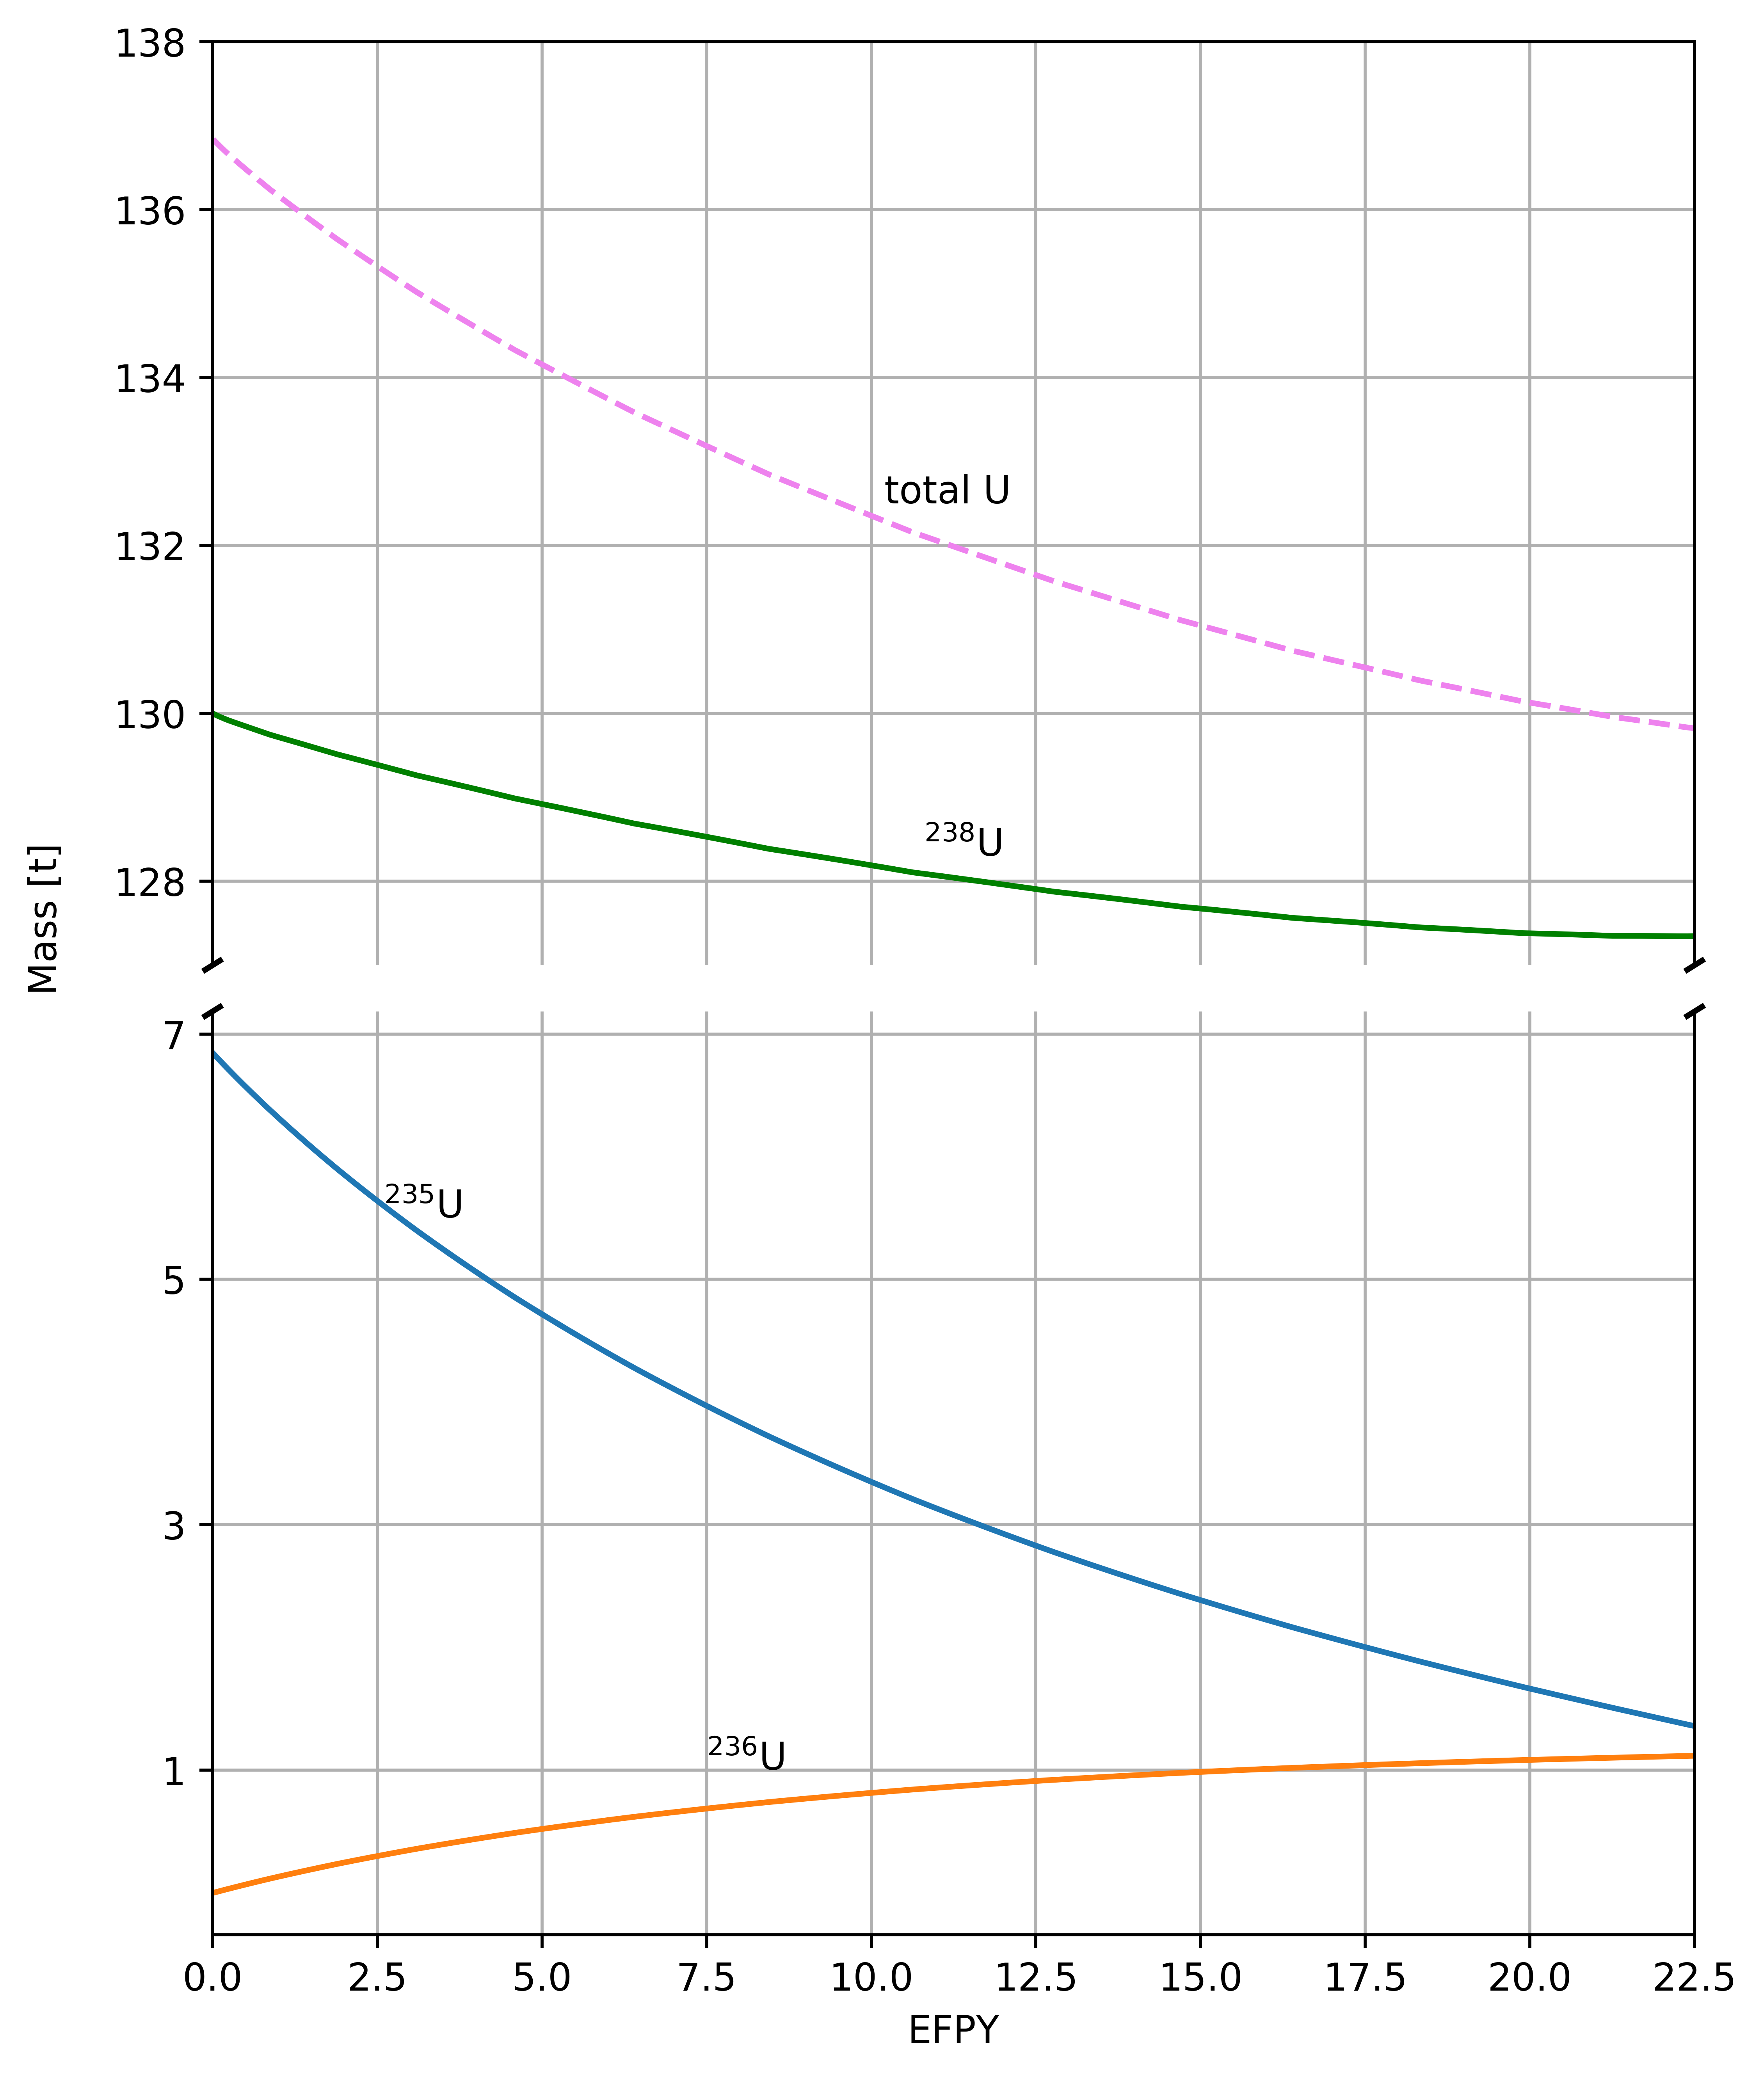
\includegraphics[width=\textwidth]{ch4/u_ben_valid.png}
	\caption{SaltProc-calculated uranium isotopic fuel salt content during 
	22.5 years of operation.}
	\label{fig:u-ben-valid}
\end{figure}
\begin{figure}[hbp!] % replace 't' with 'b' to 
	\centering
	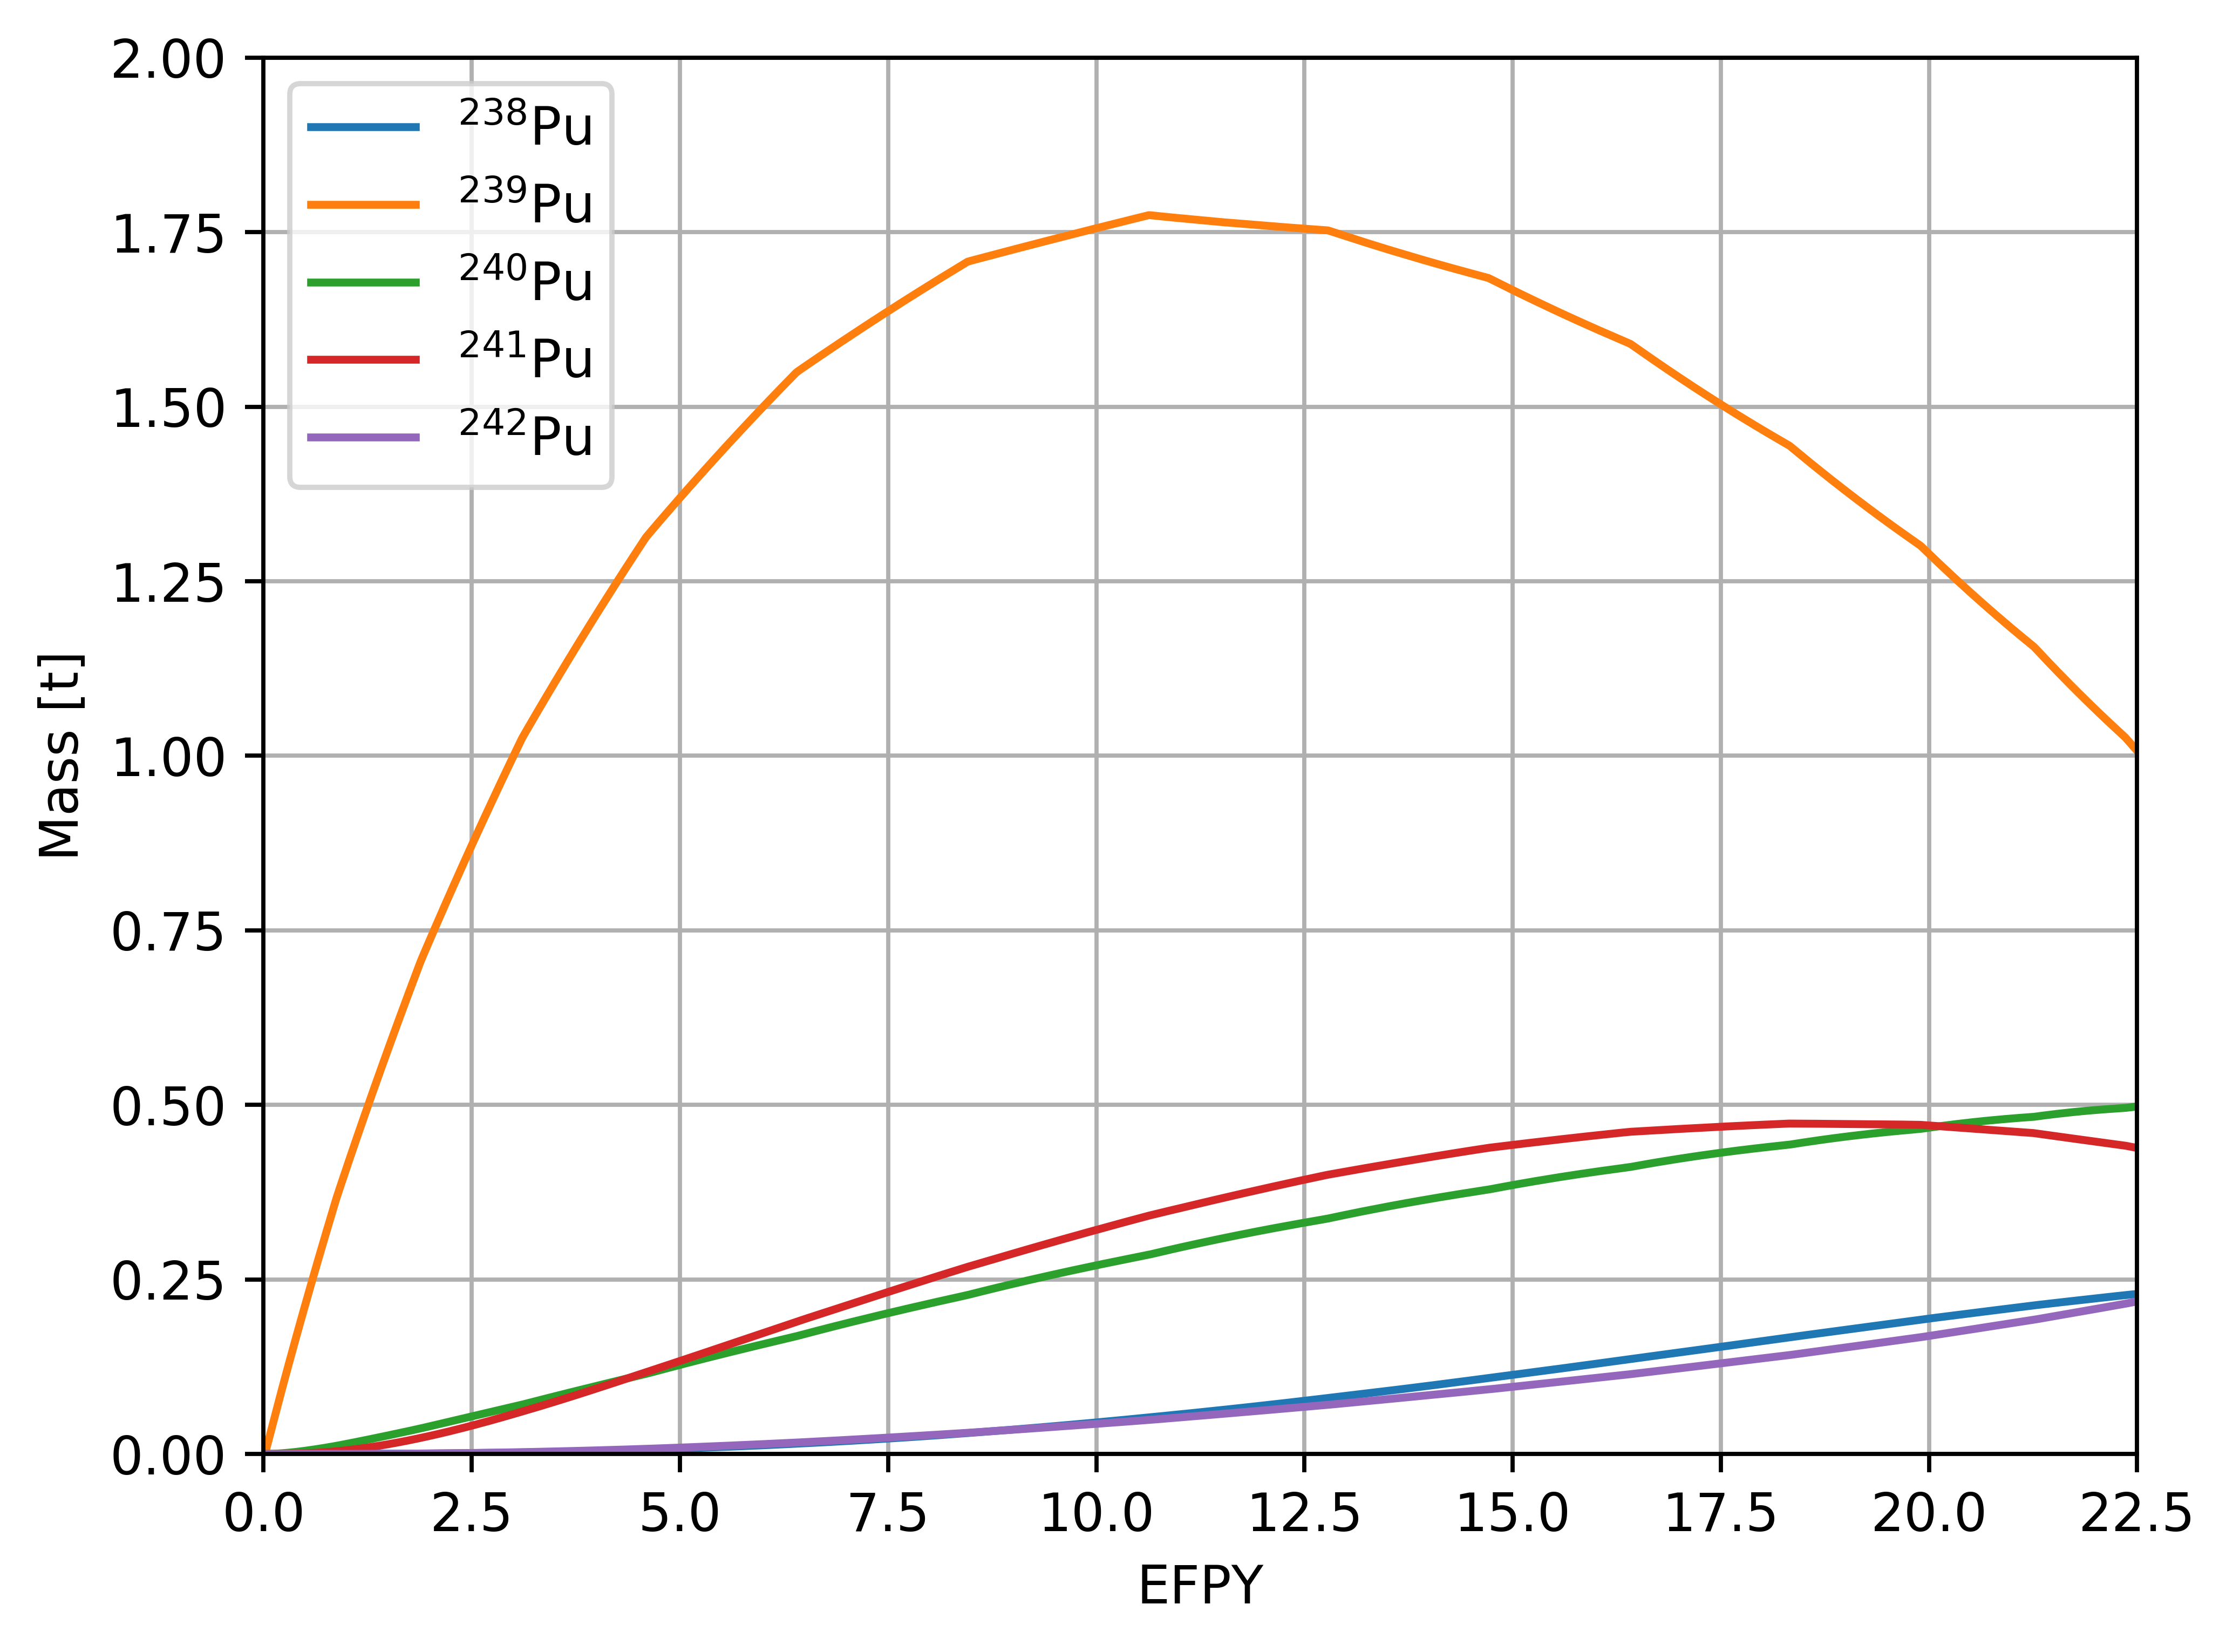
\includegraphics[width=\textwidth]{ch4/pu_ben_valid.png}
	\caption{SaltProc-calculated plutonium isotopic fuel salt content during 
		22.5 years of operation.}
	\label{fig:pu-ben-valid}
\end{figure}

\begin{figure}[hbp!] % replace 't' with 'b' to 
	\centering
	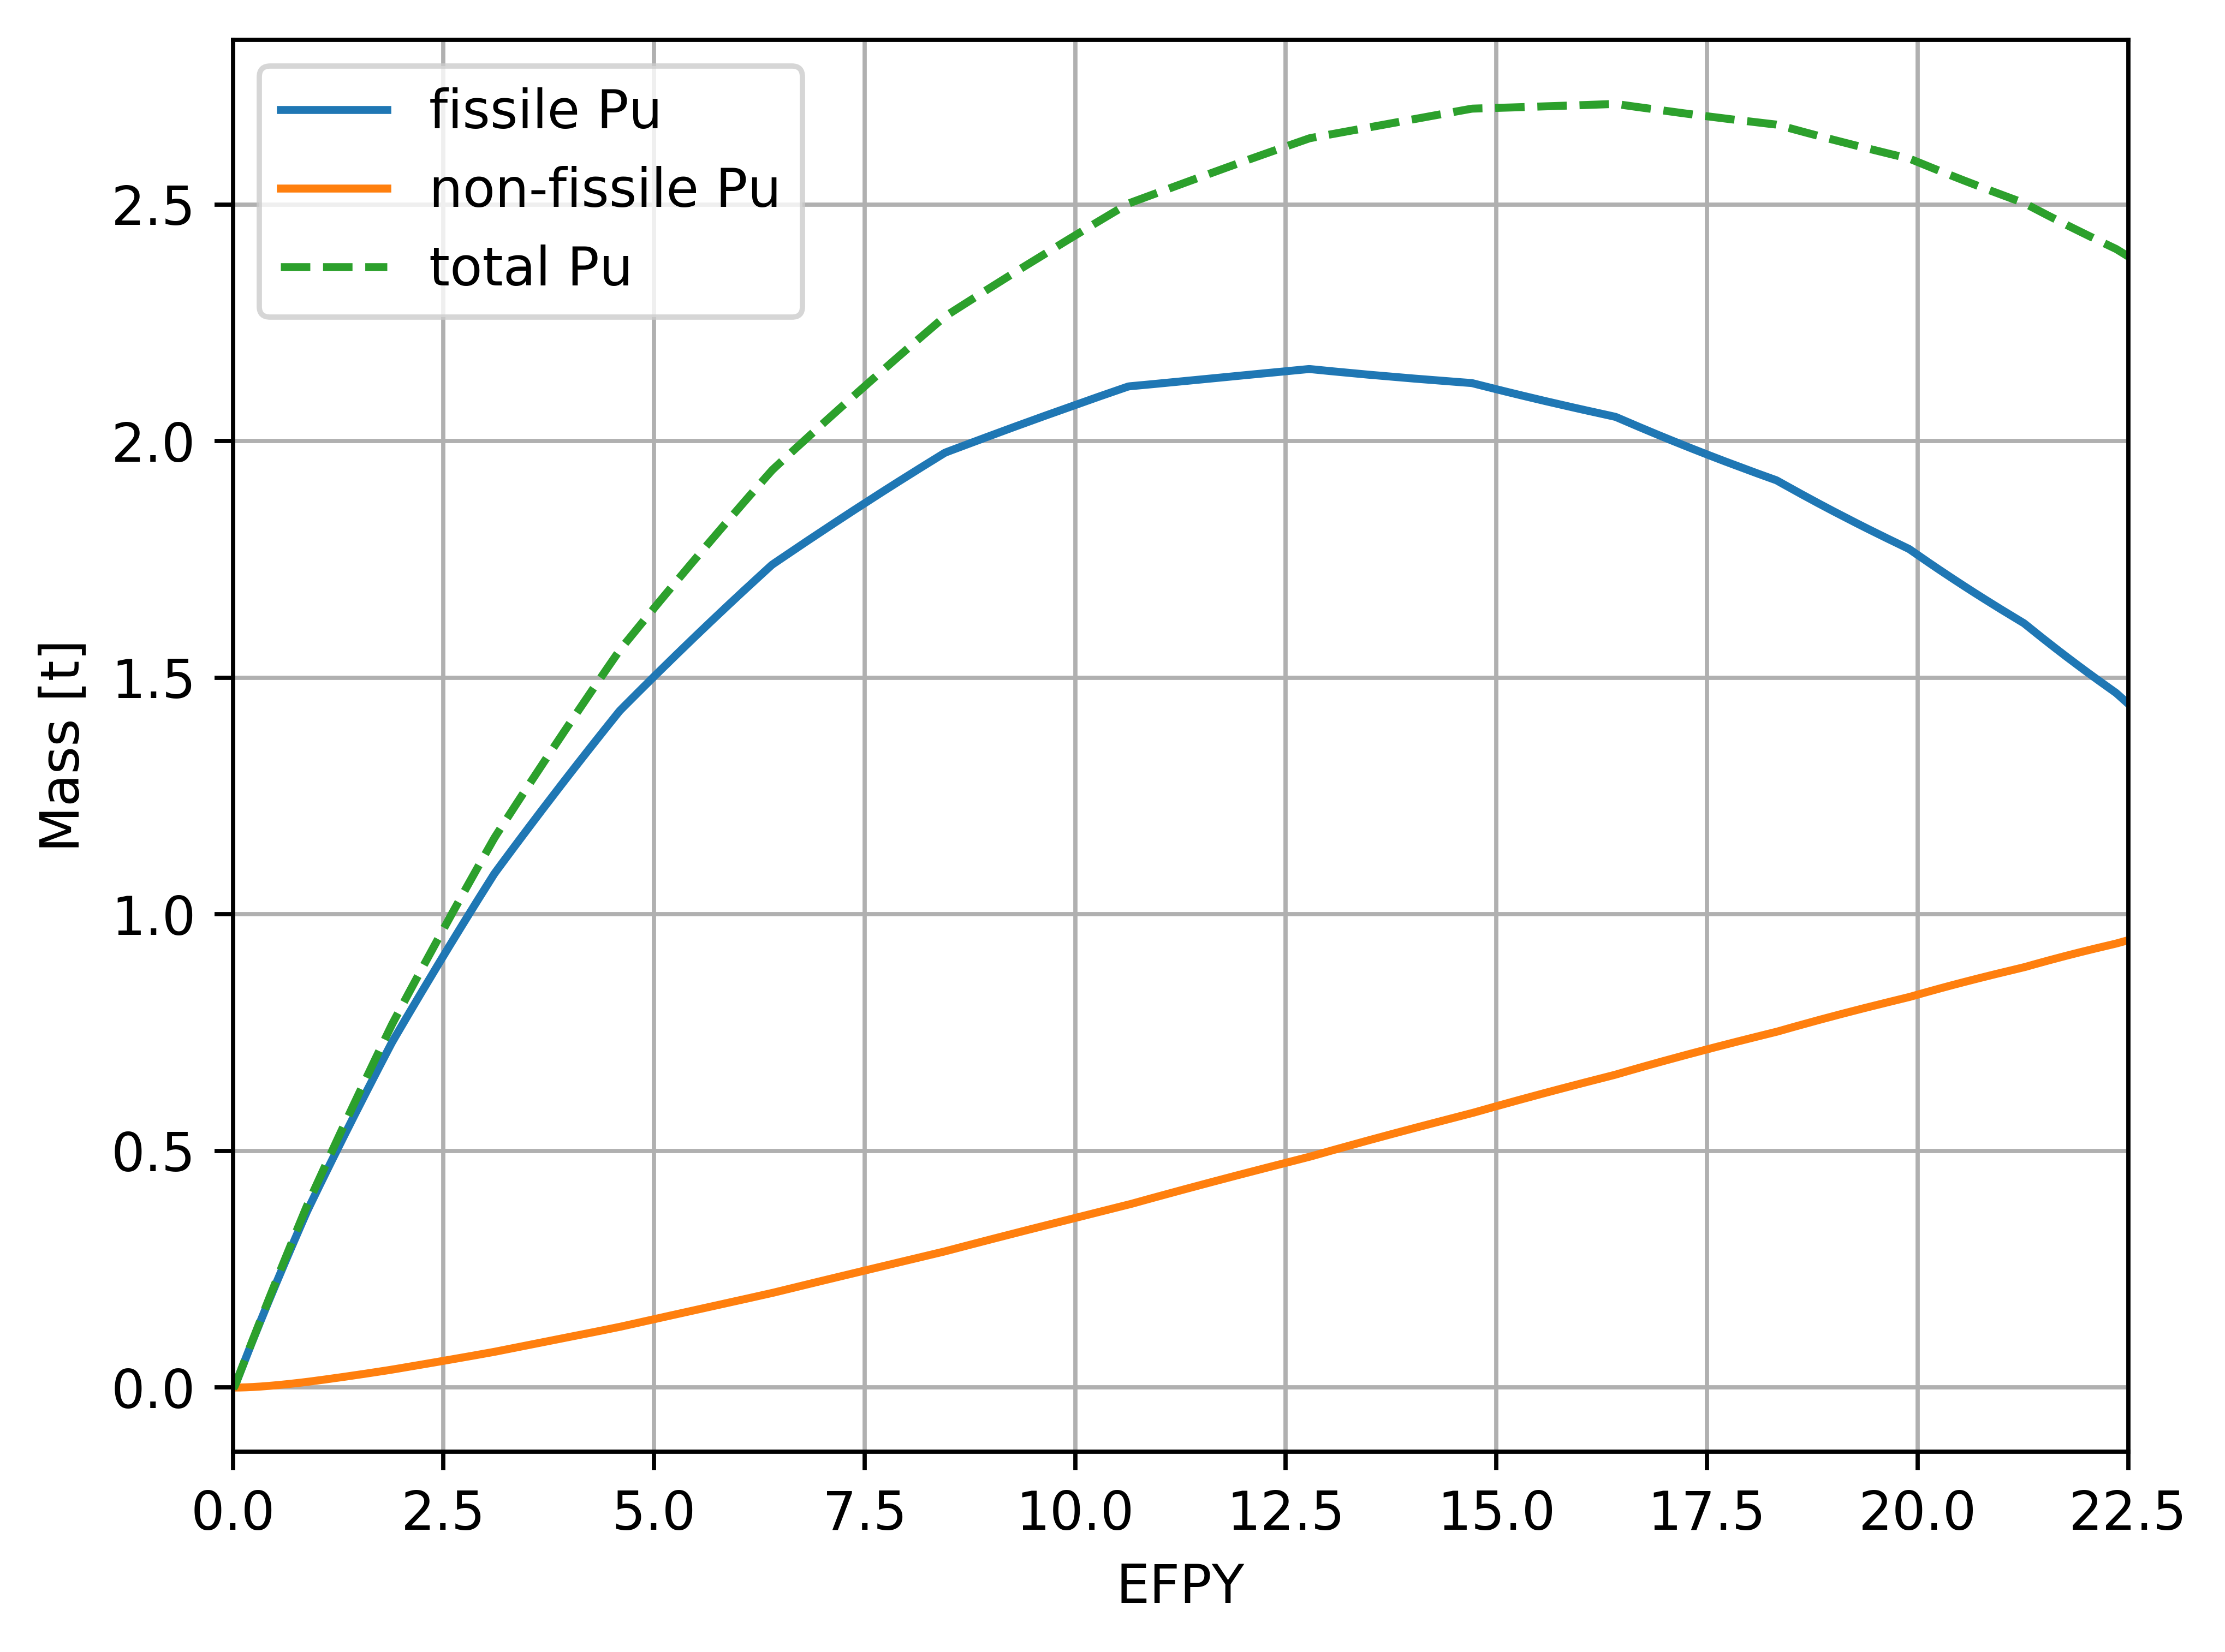
\includegraphics[width=\textwidth]{ch4/tot_pu_ben_valid.png}
	\caption{SaltProc-calculated fissile and non-fissile plutonium fuel salt 
	content during 22.5 years of operation.}
	\label{fig:pu-fiss-ben-valid}
\end{figure}
%%%%%%%%%%%%%%%%%%%%%%%%%%%%%%%%%%%%%%%%
\begin{table}[hbp!]
	\centering
	\caption{Comparison of major heavy isotopes inventories at the \gls{EOL} 
	in the \gls{TAP} reactor between the current work and Betzler \emph{et al.}	
	\cite{betzler_assessment_2017-1}.}
	\begin{tabularx}{\textwidth}{L p{0.12\textwidth} R R R}
		\hline
		& \textbf{Isotope}  & \textbf{Current work [kg]} & \textbf{Betzler, 
		2017 [kg]} & \textbf{$\Delta m$ [\%]}\\ \hline
		\multirow{4}{*}{Fissile}
		&$^{235}$U  & 1299 & 1160 & $+11$\% \\
		&$^{239}$Pu & 942  & 995  & $-5$\% \\
		&$^{241}$Pu & 427  & 435  & $-2$\% \\
		&Total & 2668 & 2590 & $+3$\%  \\ \hline
		
		\multirow{4}{*}{Non-fissile}
		&$^{236}$U  & 1123 & 1200 & $-6$\% \\
		&$^{238}$U  & 127'353 & 132'400 & $-4$\% \\
		&$^{238}$Pu & 235  & 280  & $-16$\% \\
		&$^{240}$Pu & 503  & 1000  & $-50$\% \\
		&$^{242}$Pu & 230  & 310  & $-26$\% \\
		&Total & 129'444 & 135'190 & $+4$\%  \\ \hline
	\end{tabularx}
	\label{tab:valid_ben_isos}
	\vspace{-0.9em}
\end{table}
%%%%%%%%%%%%%%%%%%%%%%%%%%%%%%%%%%%%%%%%%%%%%%%%%%%%%%%%%%%%%%%%%%%%%%%%%%%%%%%

Lifetime-long SaltProc calculation requires a 5\% \gls{LEU} feed rate of 460.8 
kg per year to maintain the fuel salt inventory in the primary loop which is 
consistent with the reference. Table~\ref{tab:valid_ben_performance} shows 
main fuel cycle performance parameters calculated using SaltProc and compared 
with the reference. Normalized per GW$_{th}$-year, the \gls{TAP} concept 
requires about 5.23 t of fuel compared with 4.14 t reported by Betzler 
\emph{et al.} SaltProc-calculated waste production normalized per 
GW$_{th}$-year is 5\% less than reported by ORNL. Potentially, the \gls{TAP} 
can operate with \gls{LWR} \gls{SNF} as the fissile material feed. The heavy 
metal component of \gls{LWR} \gls{SNF} has a lower fissile material weight 
fraction than 5\% enriched uranium and adds less fertile $^{238}$U to the fuel 
salt, potentially reducing the operational lifetime. But in case of using 
waste material (e.g., Transuranium elements from \gls{LWR} \gls{SNF}) in this 
fueling scenario, the \gls{TAP} concept has the potential to have a better 
waste reduction metrics.
%%%%%%%%%%%%%%%%%%%%%%%%%%%%%%%%%%%%%%%%
\begin{table}[hbp!]
	\centering
	\caption{Comparison of normalized total fuel load and actinide waste from 
	the TAP reactor obtained in the current work and Betzler \emph{et al.} 
	\cite{betzler_assessment_2017-1}.}
	\begin{tabularx}{\textwidth}{p{0.42\textwidth} R R}
		\hline
		\textbf{Parameter}  & \textbf{Current work} & \textbf{Betzler, 2017} 
		\cite{betzler_assessment_2017-1}\\ \hline
		5\% \gls{LEU} feed rate [kg/y] & 460.8 & 480.0 \\
		Loaded fuel [MT per GW$_{th}$-y] & 5.23 & 4.14 \\
		Waste  [MT per GW$_{th}$-y] & 3.57 & 3.74 \\
		\hline
	\end{tabularx}
	\label{tab:valid_ben_performance}
	\vspace{-0.9em}
\end{table}
%%%%%%%%%%%%%%%%%%%%%%%%%%%%%%%%%%%%%%%%%%%%%%%%%%%%%%%%%%%%%%%%%%%%%%%%%%%%%%%

\subsubsection{Neutron energy spectrum}
Significant thermalization of the neutron spectrum is observed as moderator 
rods are added into the core configuration 
(Figure~\ref{fig:ben-spectrum-bol}). At startup, the neutron spectra from the 
current work and Betzler \emph{et al.} are match well because the core 
geometry, its \gls{SVF}, and initial fuel composition in 
these two simulation are similar. Pearson correlation  
coefficient\footnote{Pearson correlation coefficient is calculated by the 
	following formula:
	\begin{align}
	r &= \frac{\sum_{i=1}^{N} 
		(\Phi_i^{ref}-\overline{\Phi^{ref}})(\Phi_i-\overline{\Phi})}
	{\sqrt{\sum_{i=1}^{N} (\Phi_i^{ref}-\overline{\Phi^{ref}})^2 
			\sum_{i=1}^{N} 
			(\Phi_i-\overline{\Phi})^2}}\\
	\mbox{where} \nonumber\\
	\Phi_i^{ref},\Phi_i &= \mbox{neutron flux for i$^{th}$ energy bin 
		reported in the reference and the current work $[n/cm^2\cdot s]$} 
	\nonumber\\
	\overline{\Phi^{ref}}, \overline{\Phi} &= \mbox{neutron flux averaged over 
		N energy bins reported in the reference and current work $[n/cm^2\cdot 
		s]$} 
	\nonumber\\
	N &= \mbox{number of neutron energy bins [-].}
	\nonumber
	\end{align}}
$r_{BOL}=0.91115$ which indicates strong, positive association between the 
spectra at the \gls{BOL} (see Figure~\ref{fig:ben-spectrum-bol}, upper plot).
At the \gls{EOL}, SaltProc/Serpent-calculated spectrum is more thermal than 
reported by Betzler \emph{et al.} \cite{betzler_assessment_2017-1}, but 
correlation coefficient $r_{EOL}=0.90987$ shows that the spectra are still 
extremely strongly related (see Figure~\ref{fig:ben-spectrum-bol}, lower 
plot). 
%with smaller amplitude of resonances between 10$^{-5}$ and 10$^{-2}$ MeV 
%(resonance capture of neutrons by $^{238}$U).
\begin{figure}[htbp!] % replace 't' with 'b' to 
	\centering
	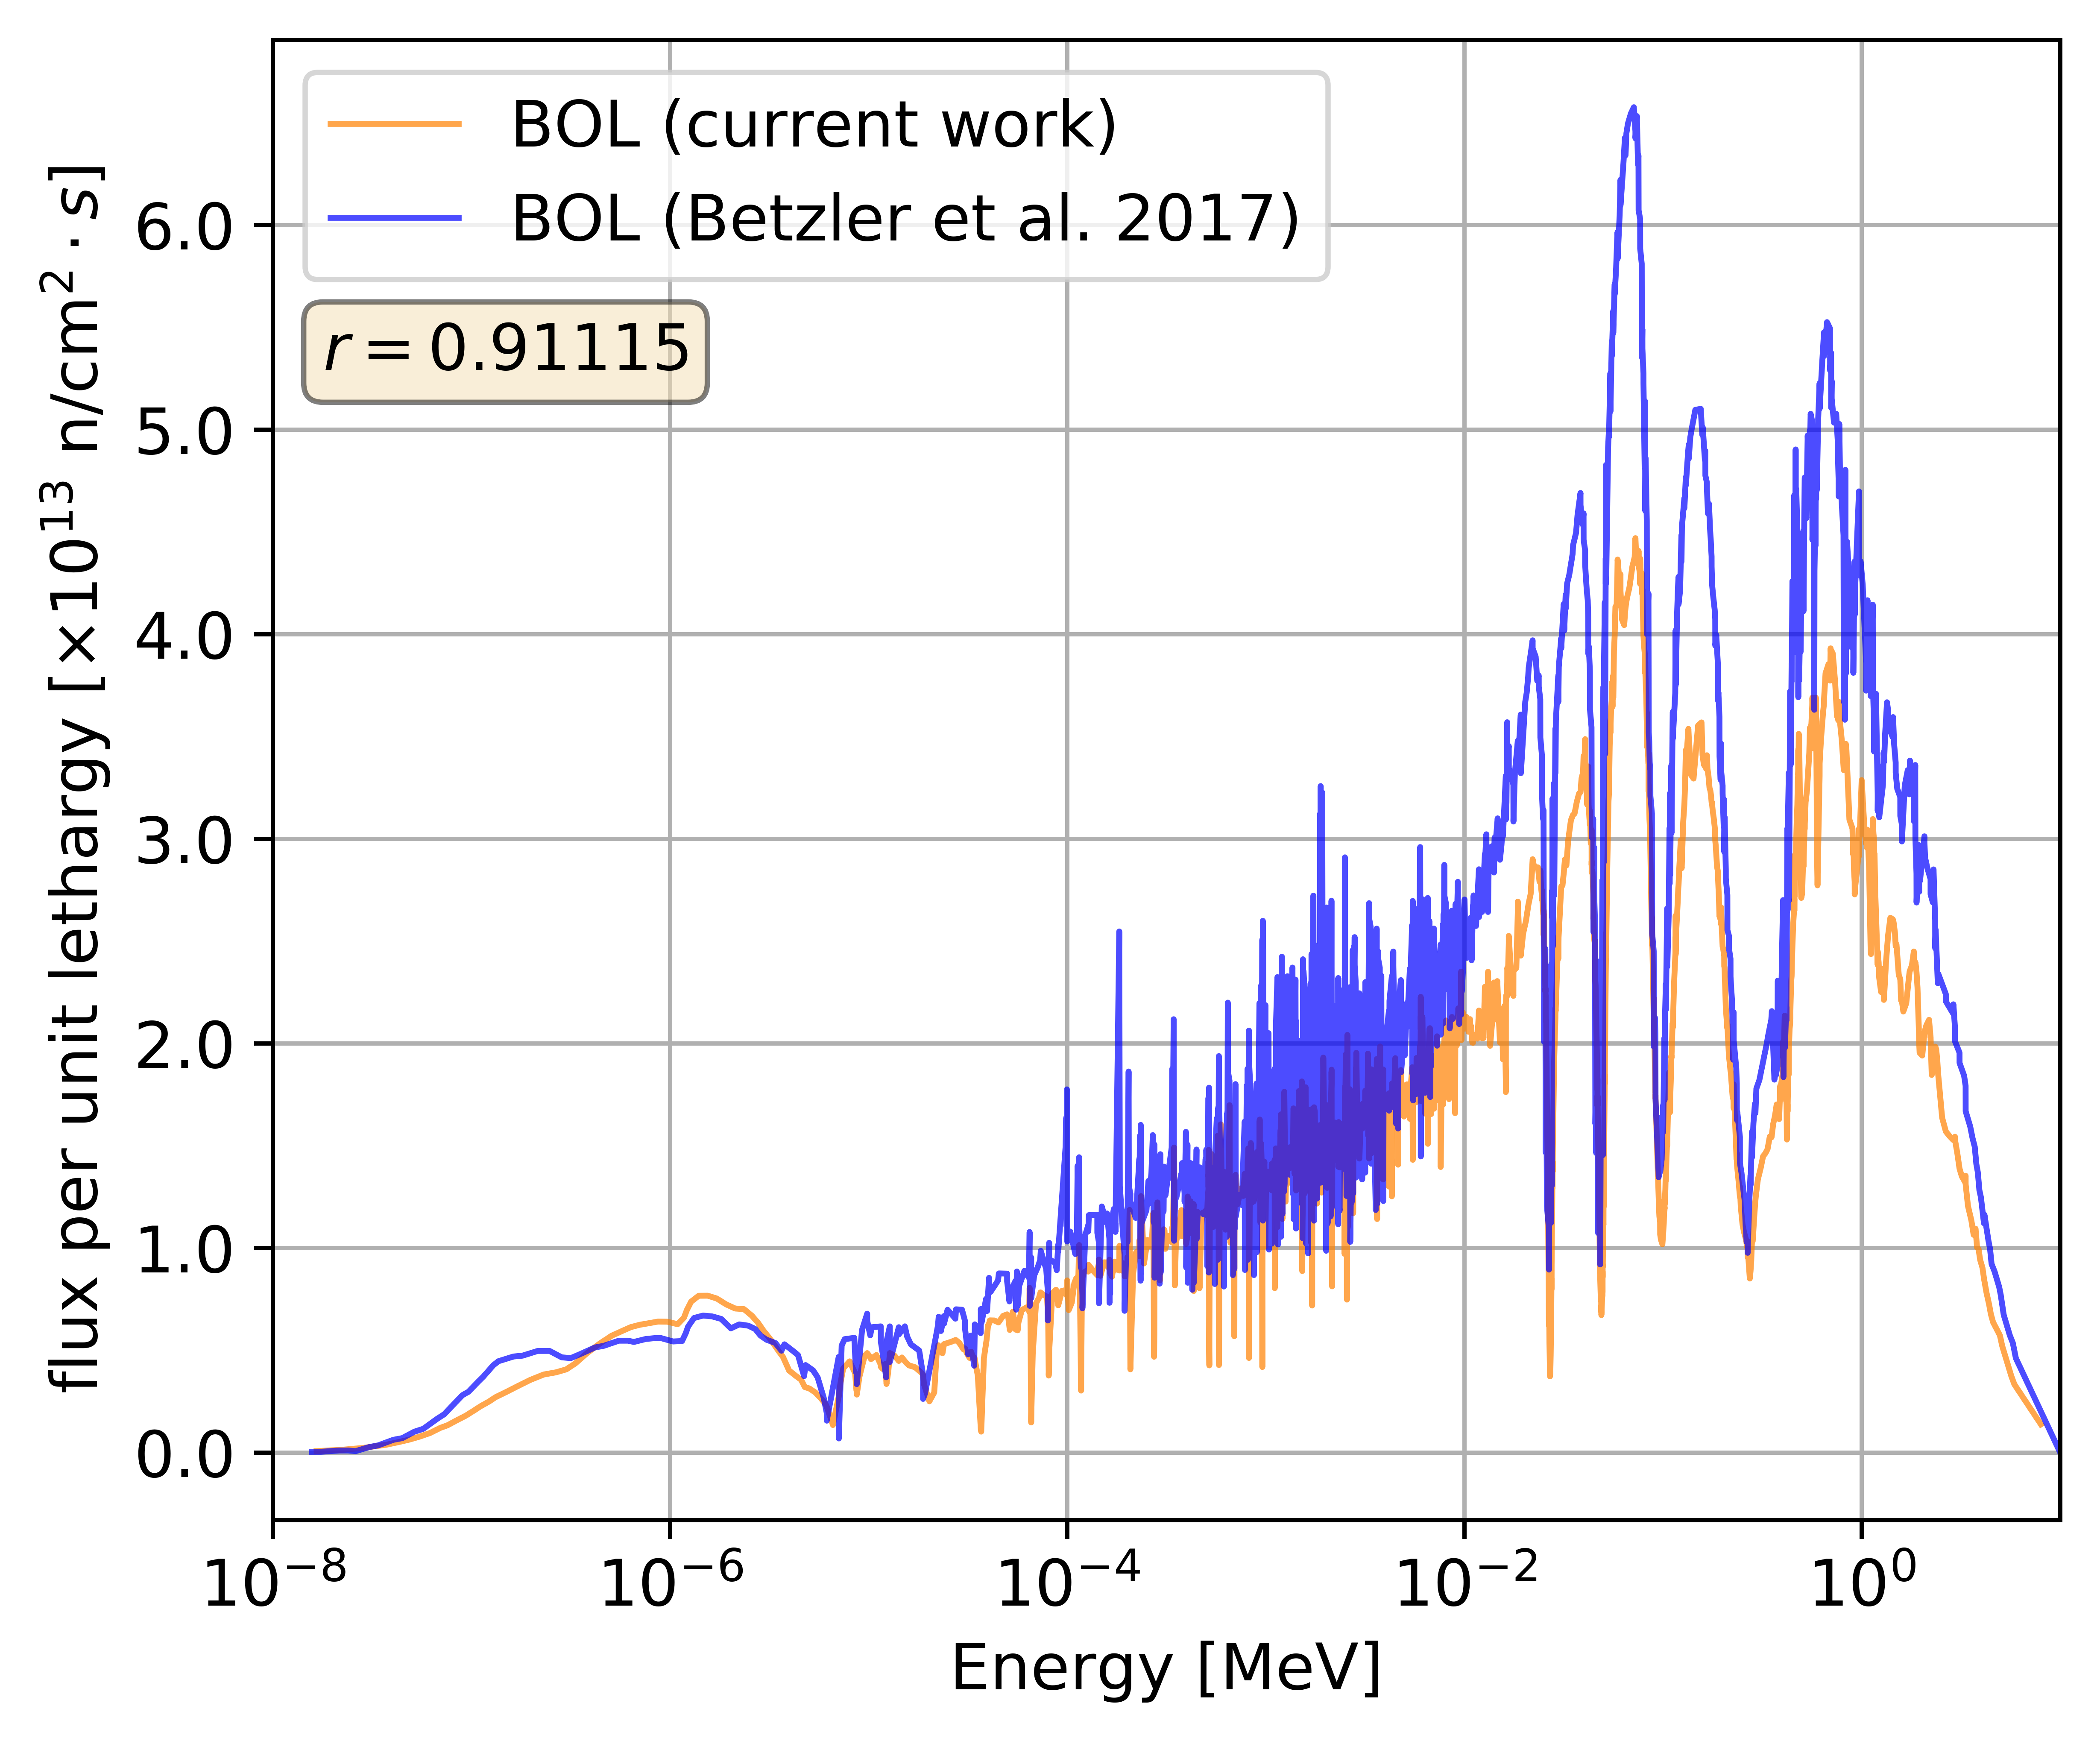
\includegraphics[width=0.77\textwidth]{ch4/ben_spec_bol.png}\\
	\vspace{-12mm}
	\hspace{0.5mm}
	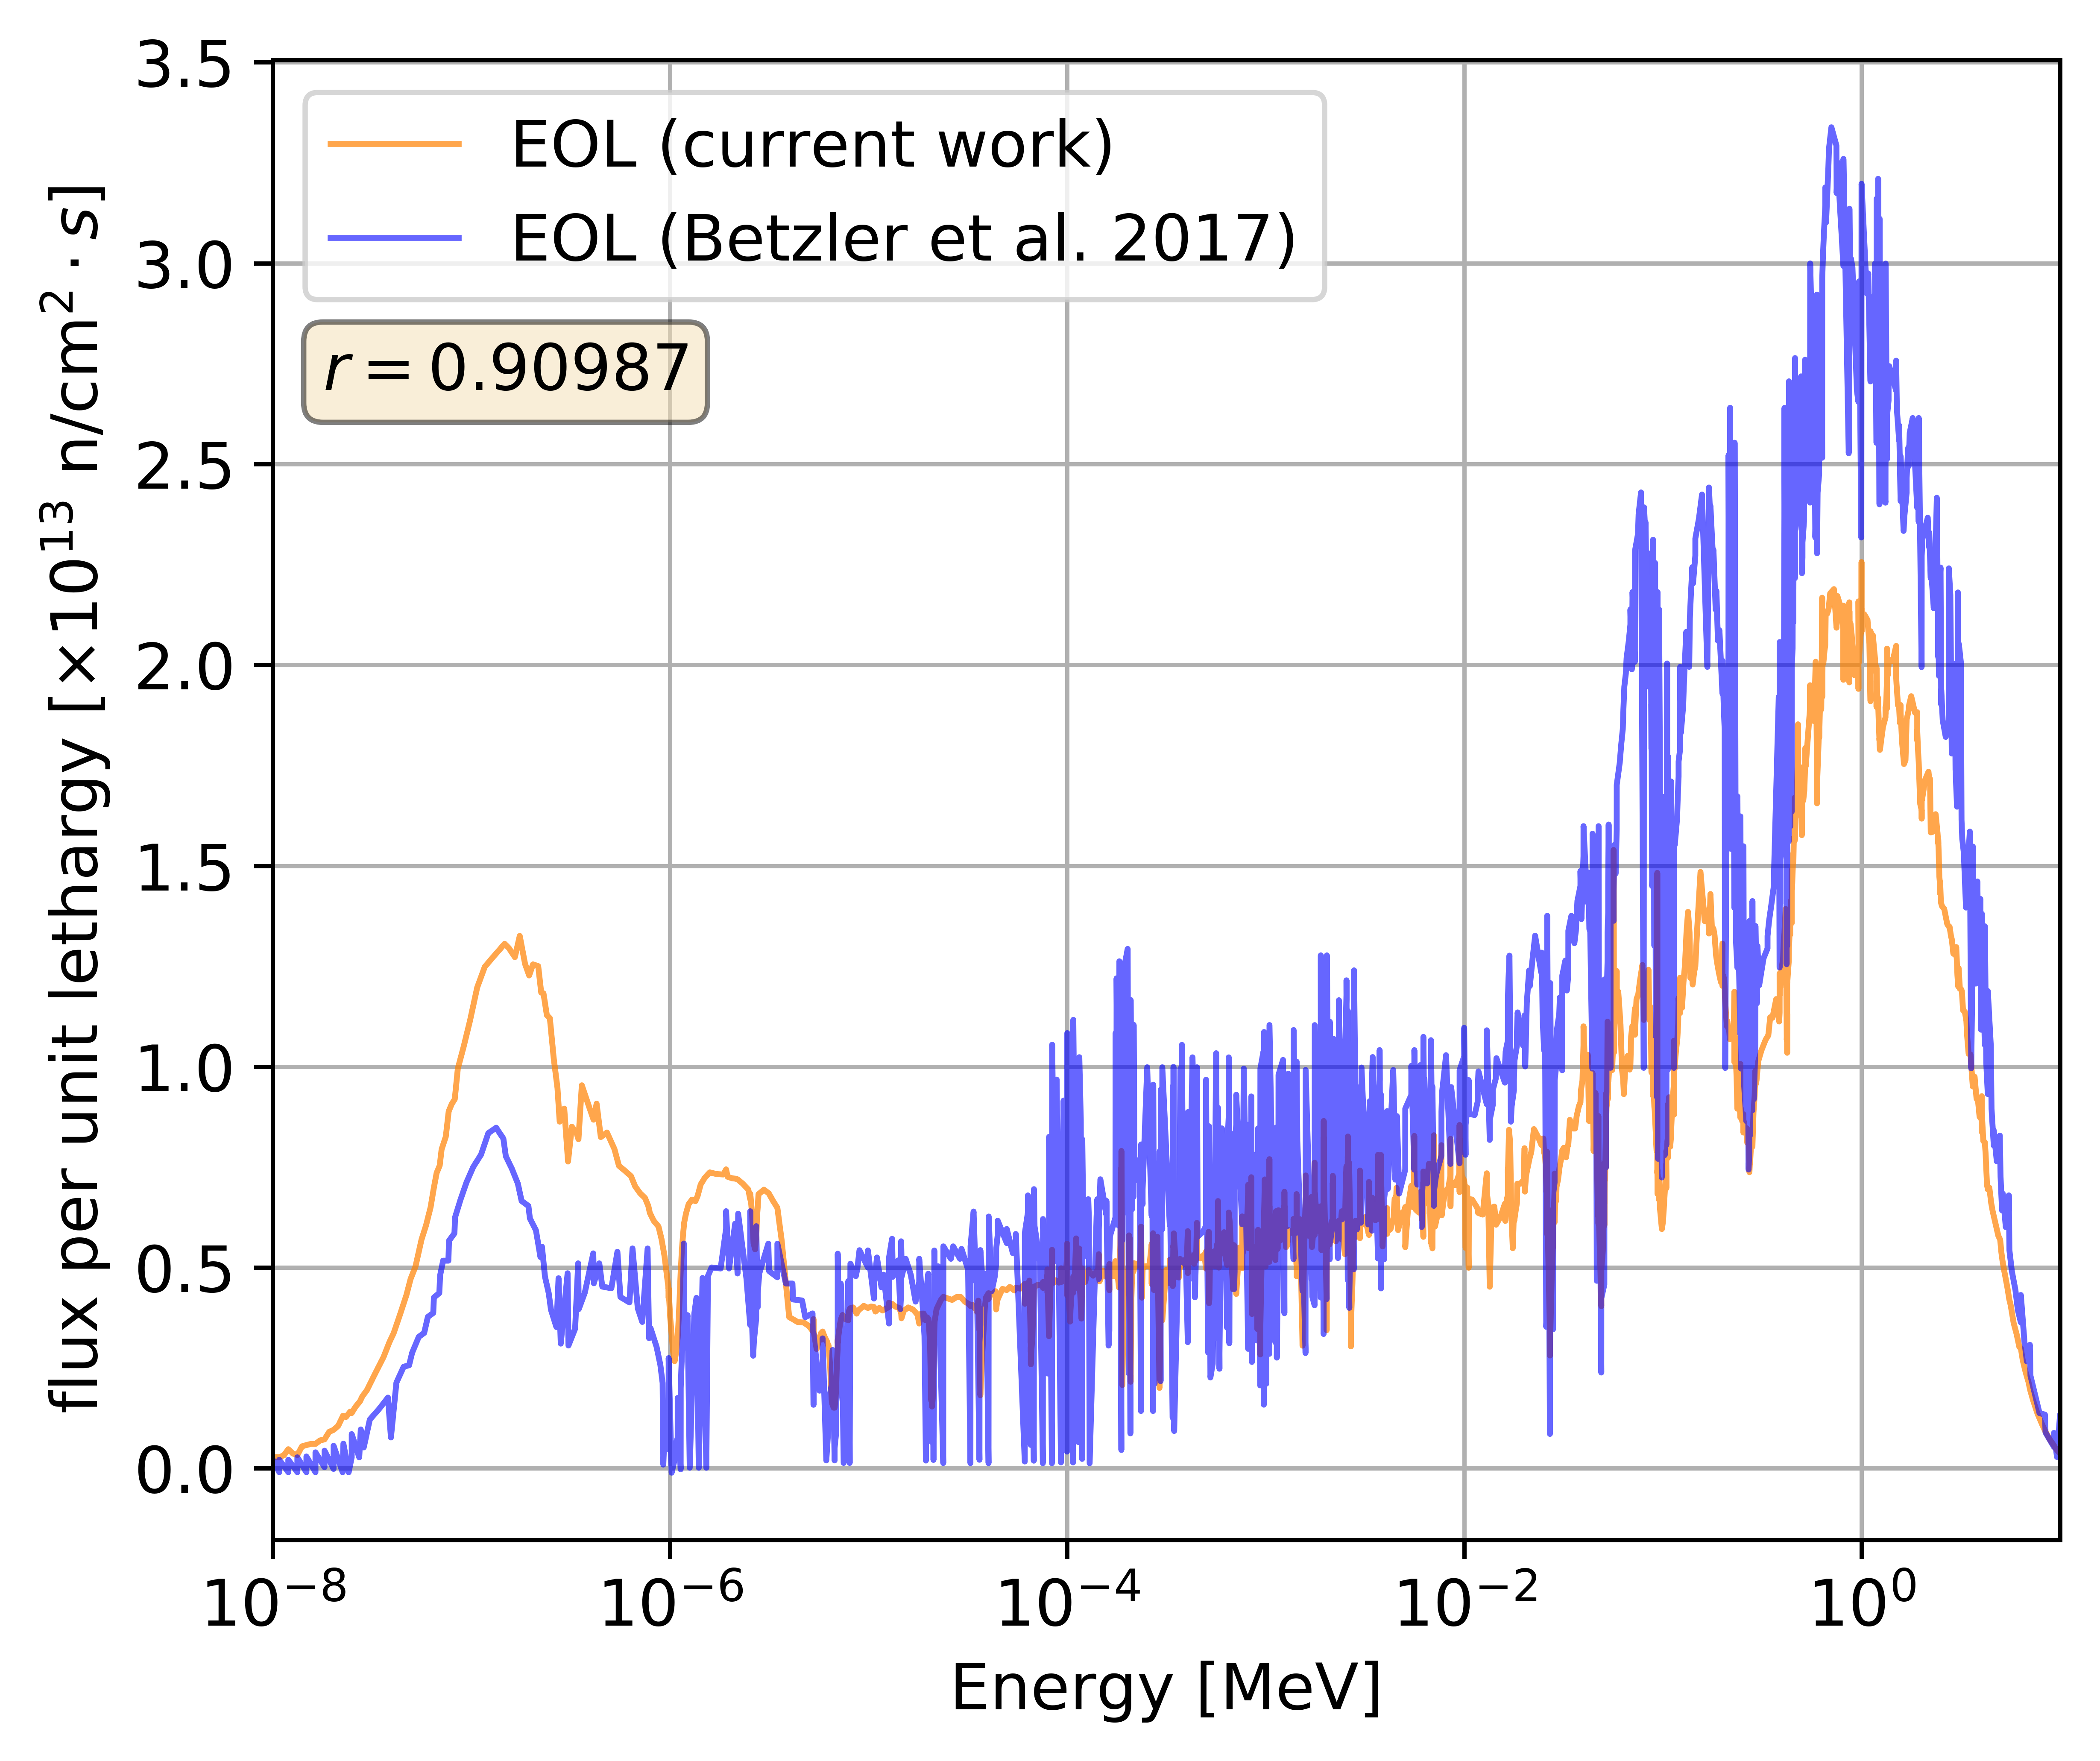
\includegraphics[width=0.77\textwidth]{ch4/ben_spec_eol.png}
	\vspace{-3mm}
	\caption{Neutron flux energy spectrum at the BOL (upper) and the EOL 
		(lower) obtained using SaltProc/Serpent (orange) compared with 
		ChemTriton/Shift (blue) \cite{betzler_assessment_2017-1}.}
	\label{fig:ben-spectrum-bol}
\end{figure}


Faster spectrum at the \gls{BOL} tends to significantly increase resonance 
absorption
in $^{238}$U and decrease the absorptions in fissile and 
construction materials. Thus, softer spectrum in the current work compared 
with Betzler \emph{et al.} led to fewer resonance captures\footnote{Energy 
range for $^{238}$U resonance neutron capture is between 10$^{-5}$ and 
10$^{-2}$ MeV.} of neutrons by $^{238}$U, hence, less $^{239}$Pu bred from 
$^{238}$U. Therefore, the SaltProc/Serpent calculation in the current work 
underpredicts the destruction (i.e., fission and capture) of $^{235}$U and 
overpredicts the destruction of $^{238}$U (see 
Table~\ref{tab:valid_ben_isos}). 
Finally, the softer neutron spectrum leds to more fissions in fissile 
plutonium isotopes ($^{239}$Pu and $^{241}$Pu) which also decreases 
non-fissile plutonium (Table~\ref{tab:valid_ben_isos}) and total actinide 
waste production (Table~\ref{tab:valid_ben_performance}).


\subsubsection{Time step refinement}\label{sec:time-refinement}
The results shown in this chapter are obtained from SaltProc calculation with 
uniform depletion time step of 3 days. The duration of the time step was 
chosen after performing parametric sweep to determine the longest depletion 
time step that provides suitable accuracy of the calculation. Larger time step 
potentially reduces the SaltProc calculation costs, providing results faster 
for lifetime-long (25-year) simulations. 

Figure~\ref{fig:timeref-keff} shows $k_{eff}$ evolution obtained with 3-, 6-, 
12-, and 24-days depletion time intervals for 25-year simulation. The interval 
between moderator configuration updates was assumed similar for all four cases 
for consistency. Multiplication factor at the \gls{BOC} for each moderator 
configuration became lower when the time step increasing. At the \gls{EOC} for 
each geometry, $k_{eff}=1.0$  for 3-day time step and drops significantly 
below 1.0 when depletion interval rises. The use of longer depletion time step 
decreases $k_{eff}$ at the end of each depletion step. The decrease is because 
more poisonous \glspl{FP} (e.g., $^{135}$Xe) are produced in the core during 
longer depletion interval. With longer time steps, large concentration of 
poisons are obtained at the end of depletion step when those poisons are being 
removed, resulting in the large criticality growth. 

Figures~\ref{fig:timeref-u} and \ref{fig:timeref-pu239} show that the longer 
time steps appropriately capture uranium depletion ($<1$\% difference even for 
24-day time step), but observed difference in fissile $^{239}$Pu mass is 
significant for the depletion interval 6-days and longer ($>0.5$\% 
difference for 6-day step). Using 6-day depletion interval leads to 
overprediction of $^{239}$Pu production by 5 kg at the \gls{EOL} 
(Figure~\ref{fig:timeref-pu239}). The use of 6-day time step tends to cause an 
overprediction of total plutonium production by 9.6 kg. Notably, significant 
quantity (SQ) for plutonium currently in use by the IAEA is 8 kg ($<80$\% 
$^{238}$Pu) \cite{close_iaea_1995}. Thus, 6-day depletion interval or longer 
leads to significant error in the predicted plutonium inventory at the 
\gls{EOL} (larger than 1 SQ). 
\begin{figure}[hbp!] % replace 't' with 'b' to 
	\centering
	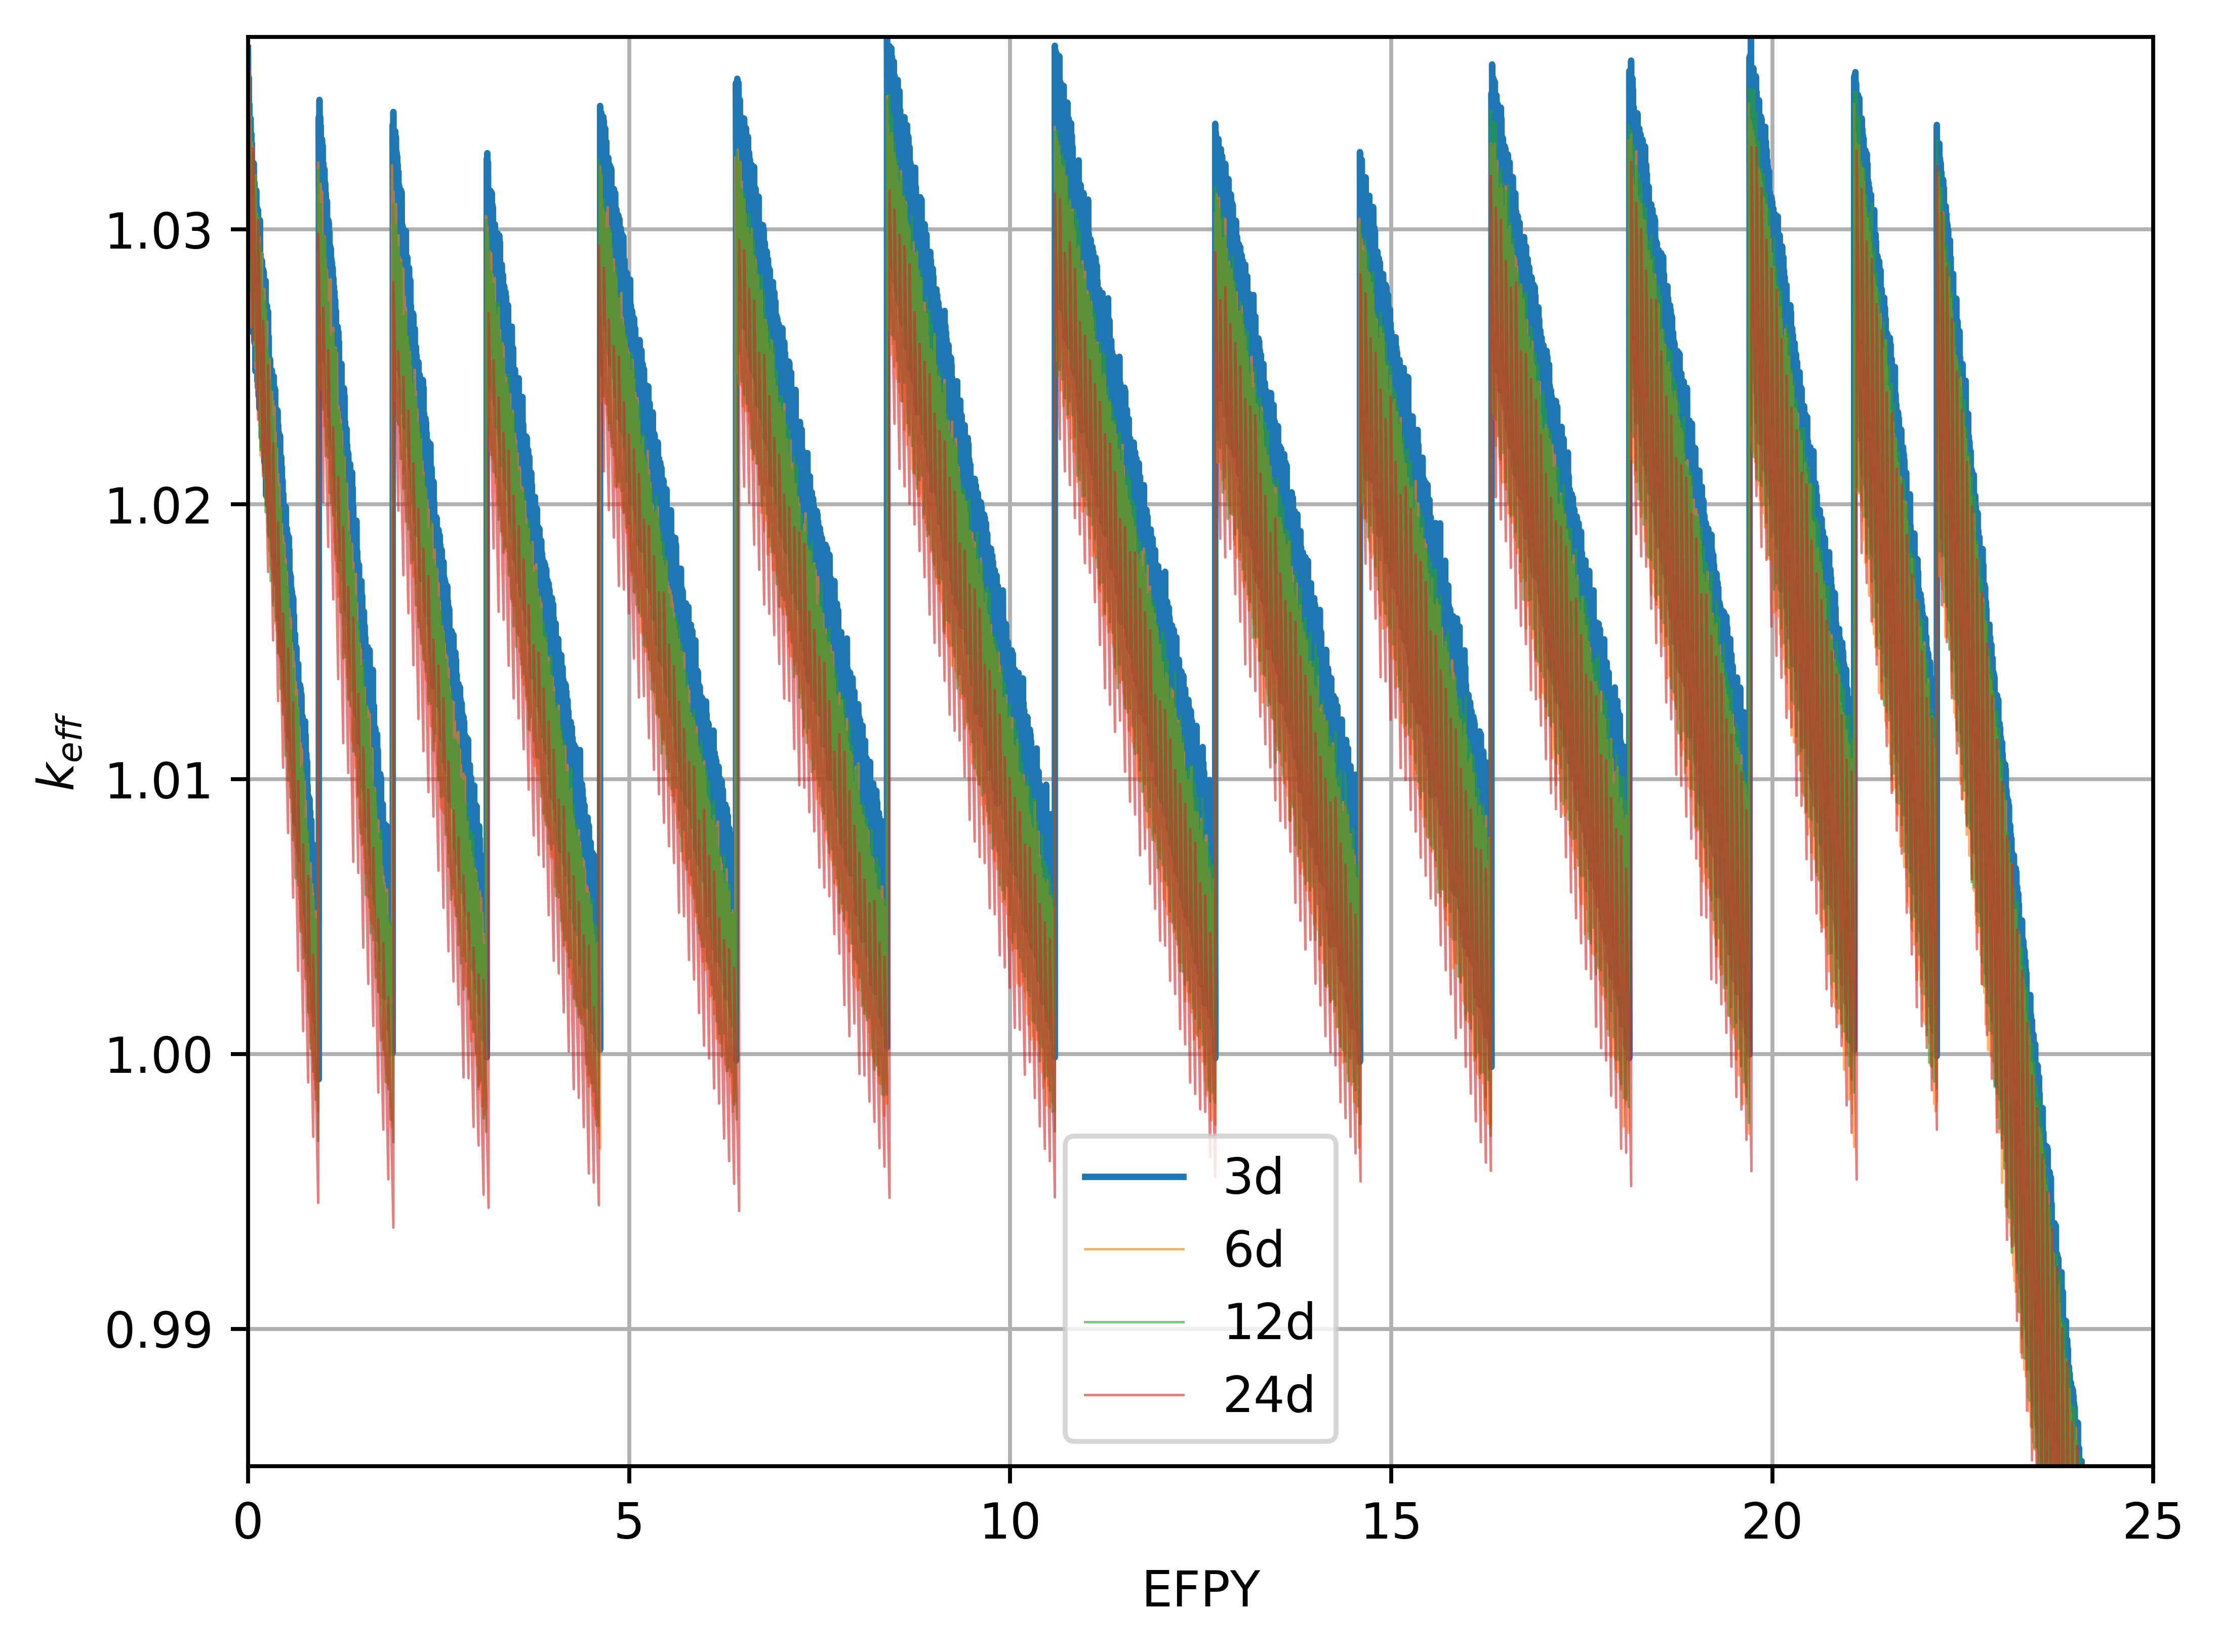
\includegraphics[width=\textwidth]{ch4/keff_time_refinement.png}
	\caption{SaltProc-calculated effective multiplication factor ($k_{eff}$) 
	during operation for different depletion time step sizes.}
	\label{fig:timeref-keff}
\end{figure}

\begin{figure}[hbp!] % replace 't' with 'b' to 
	\centering
	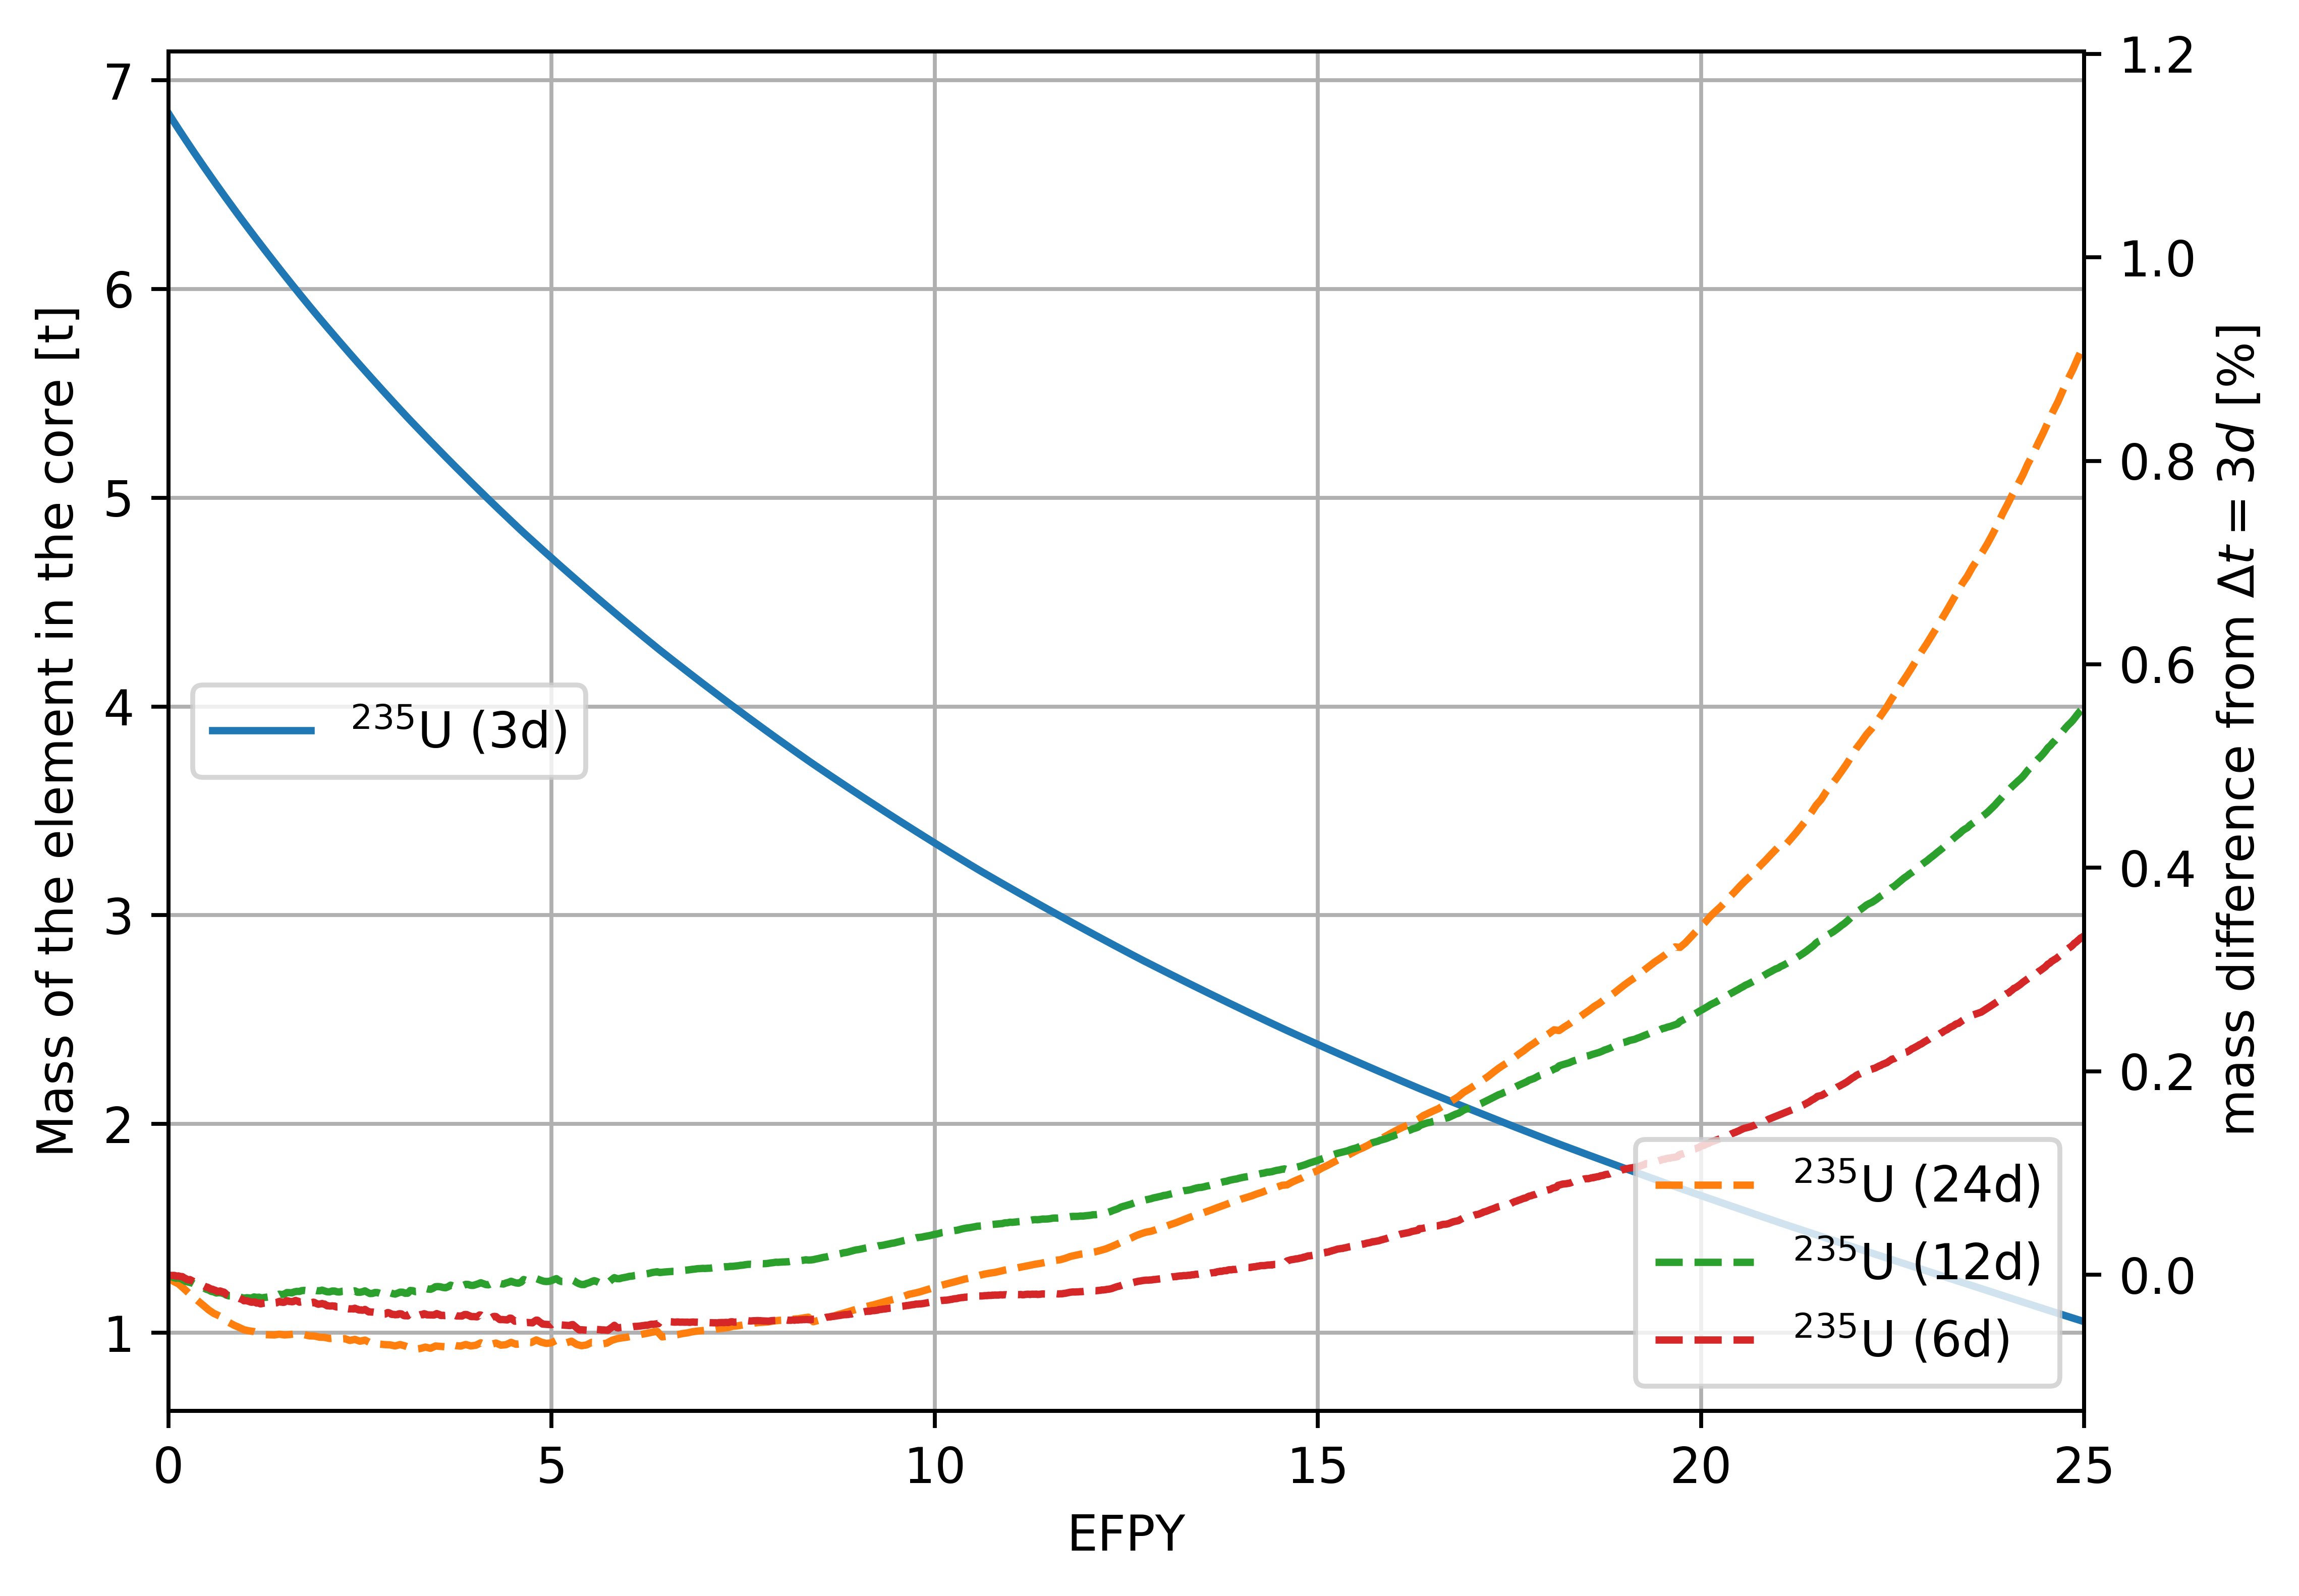
\includegraphics[width=0.91\textwidth]{ch4/u235_time_refinement.png}\\
		\vspace{-11mm}
	\hspace{0.5mm}
	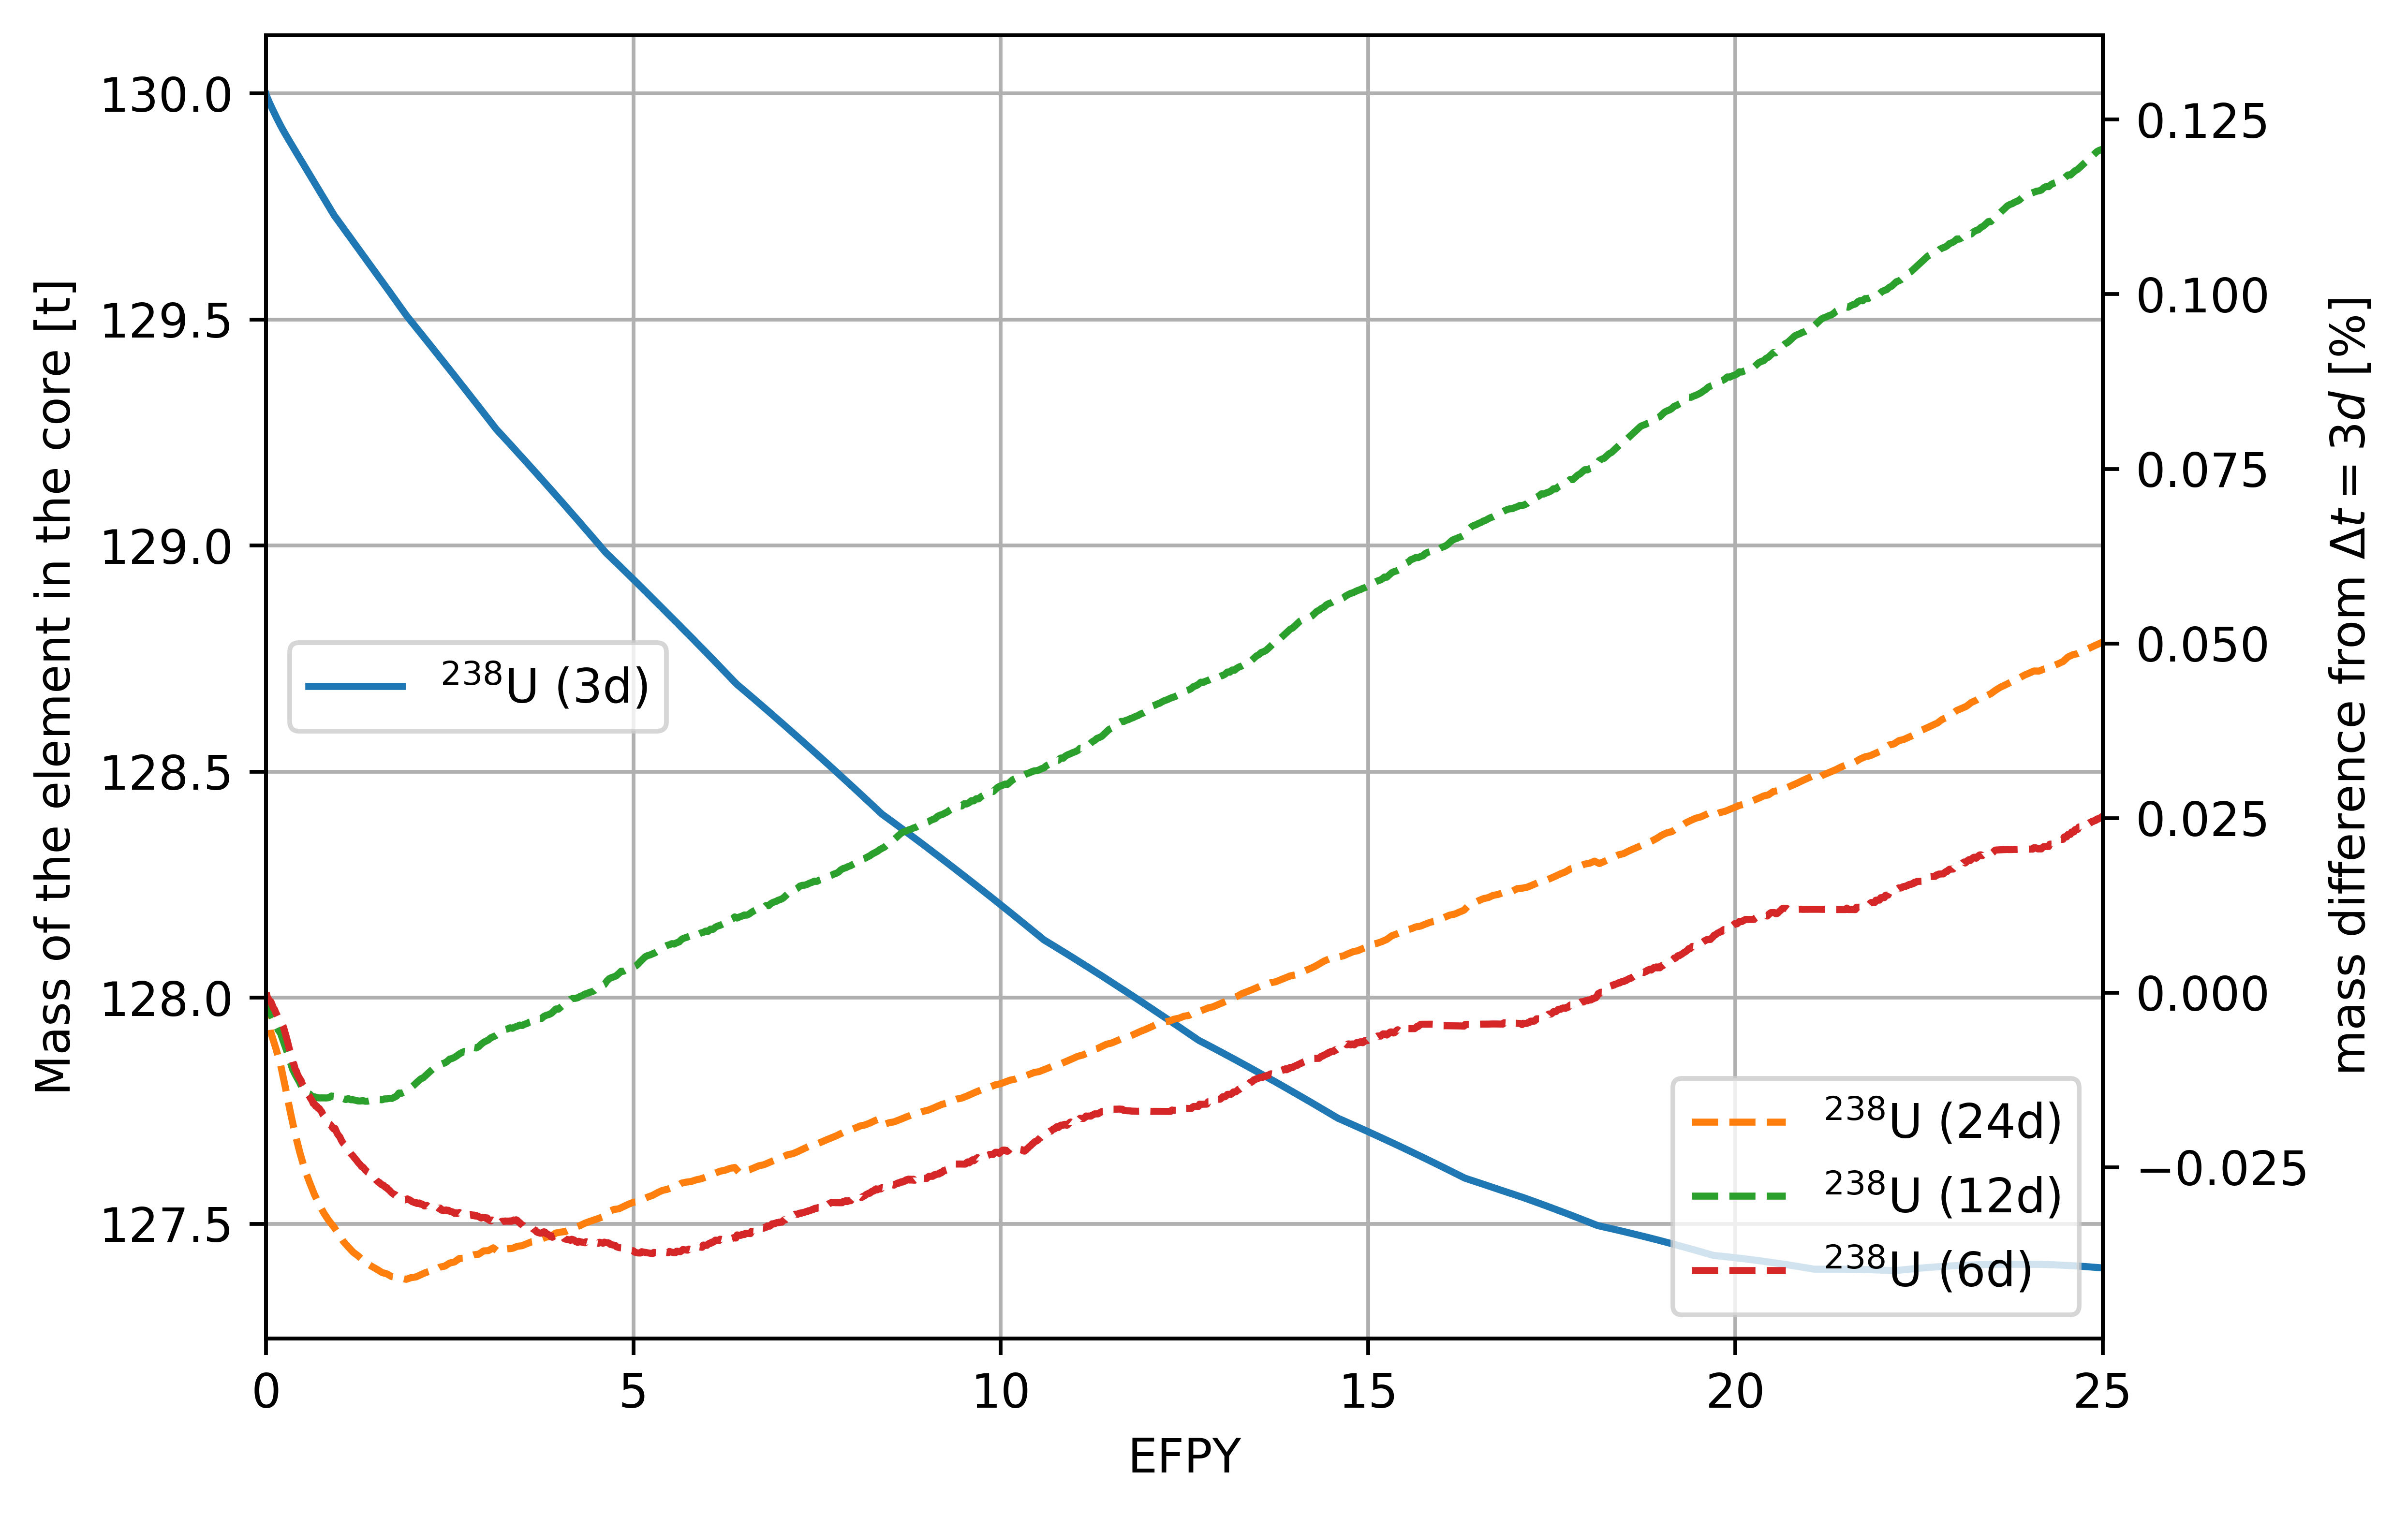
\includegraphics[width=\textwidth]{ch4/u238_time_refinement.png}
		\vspace{-6mm}
	\caption{SaltProc-calculated $^{235}$U (upper) and $^{238}$U (lower) 
	content during operation for different depletion time step sizes.}
	\label{fig:timeref-u}
\end{figure}

\begin{figure}[htp!] % replace 't' with 'b' to 
	\centering
	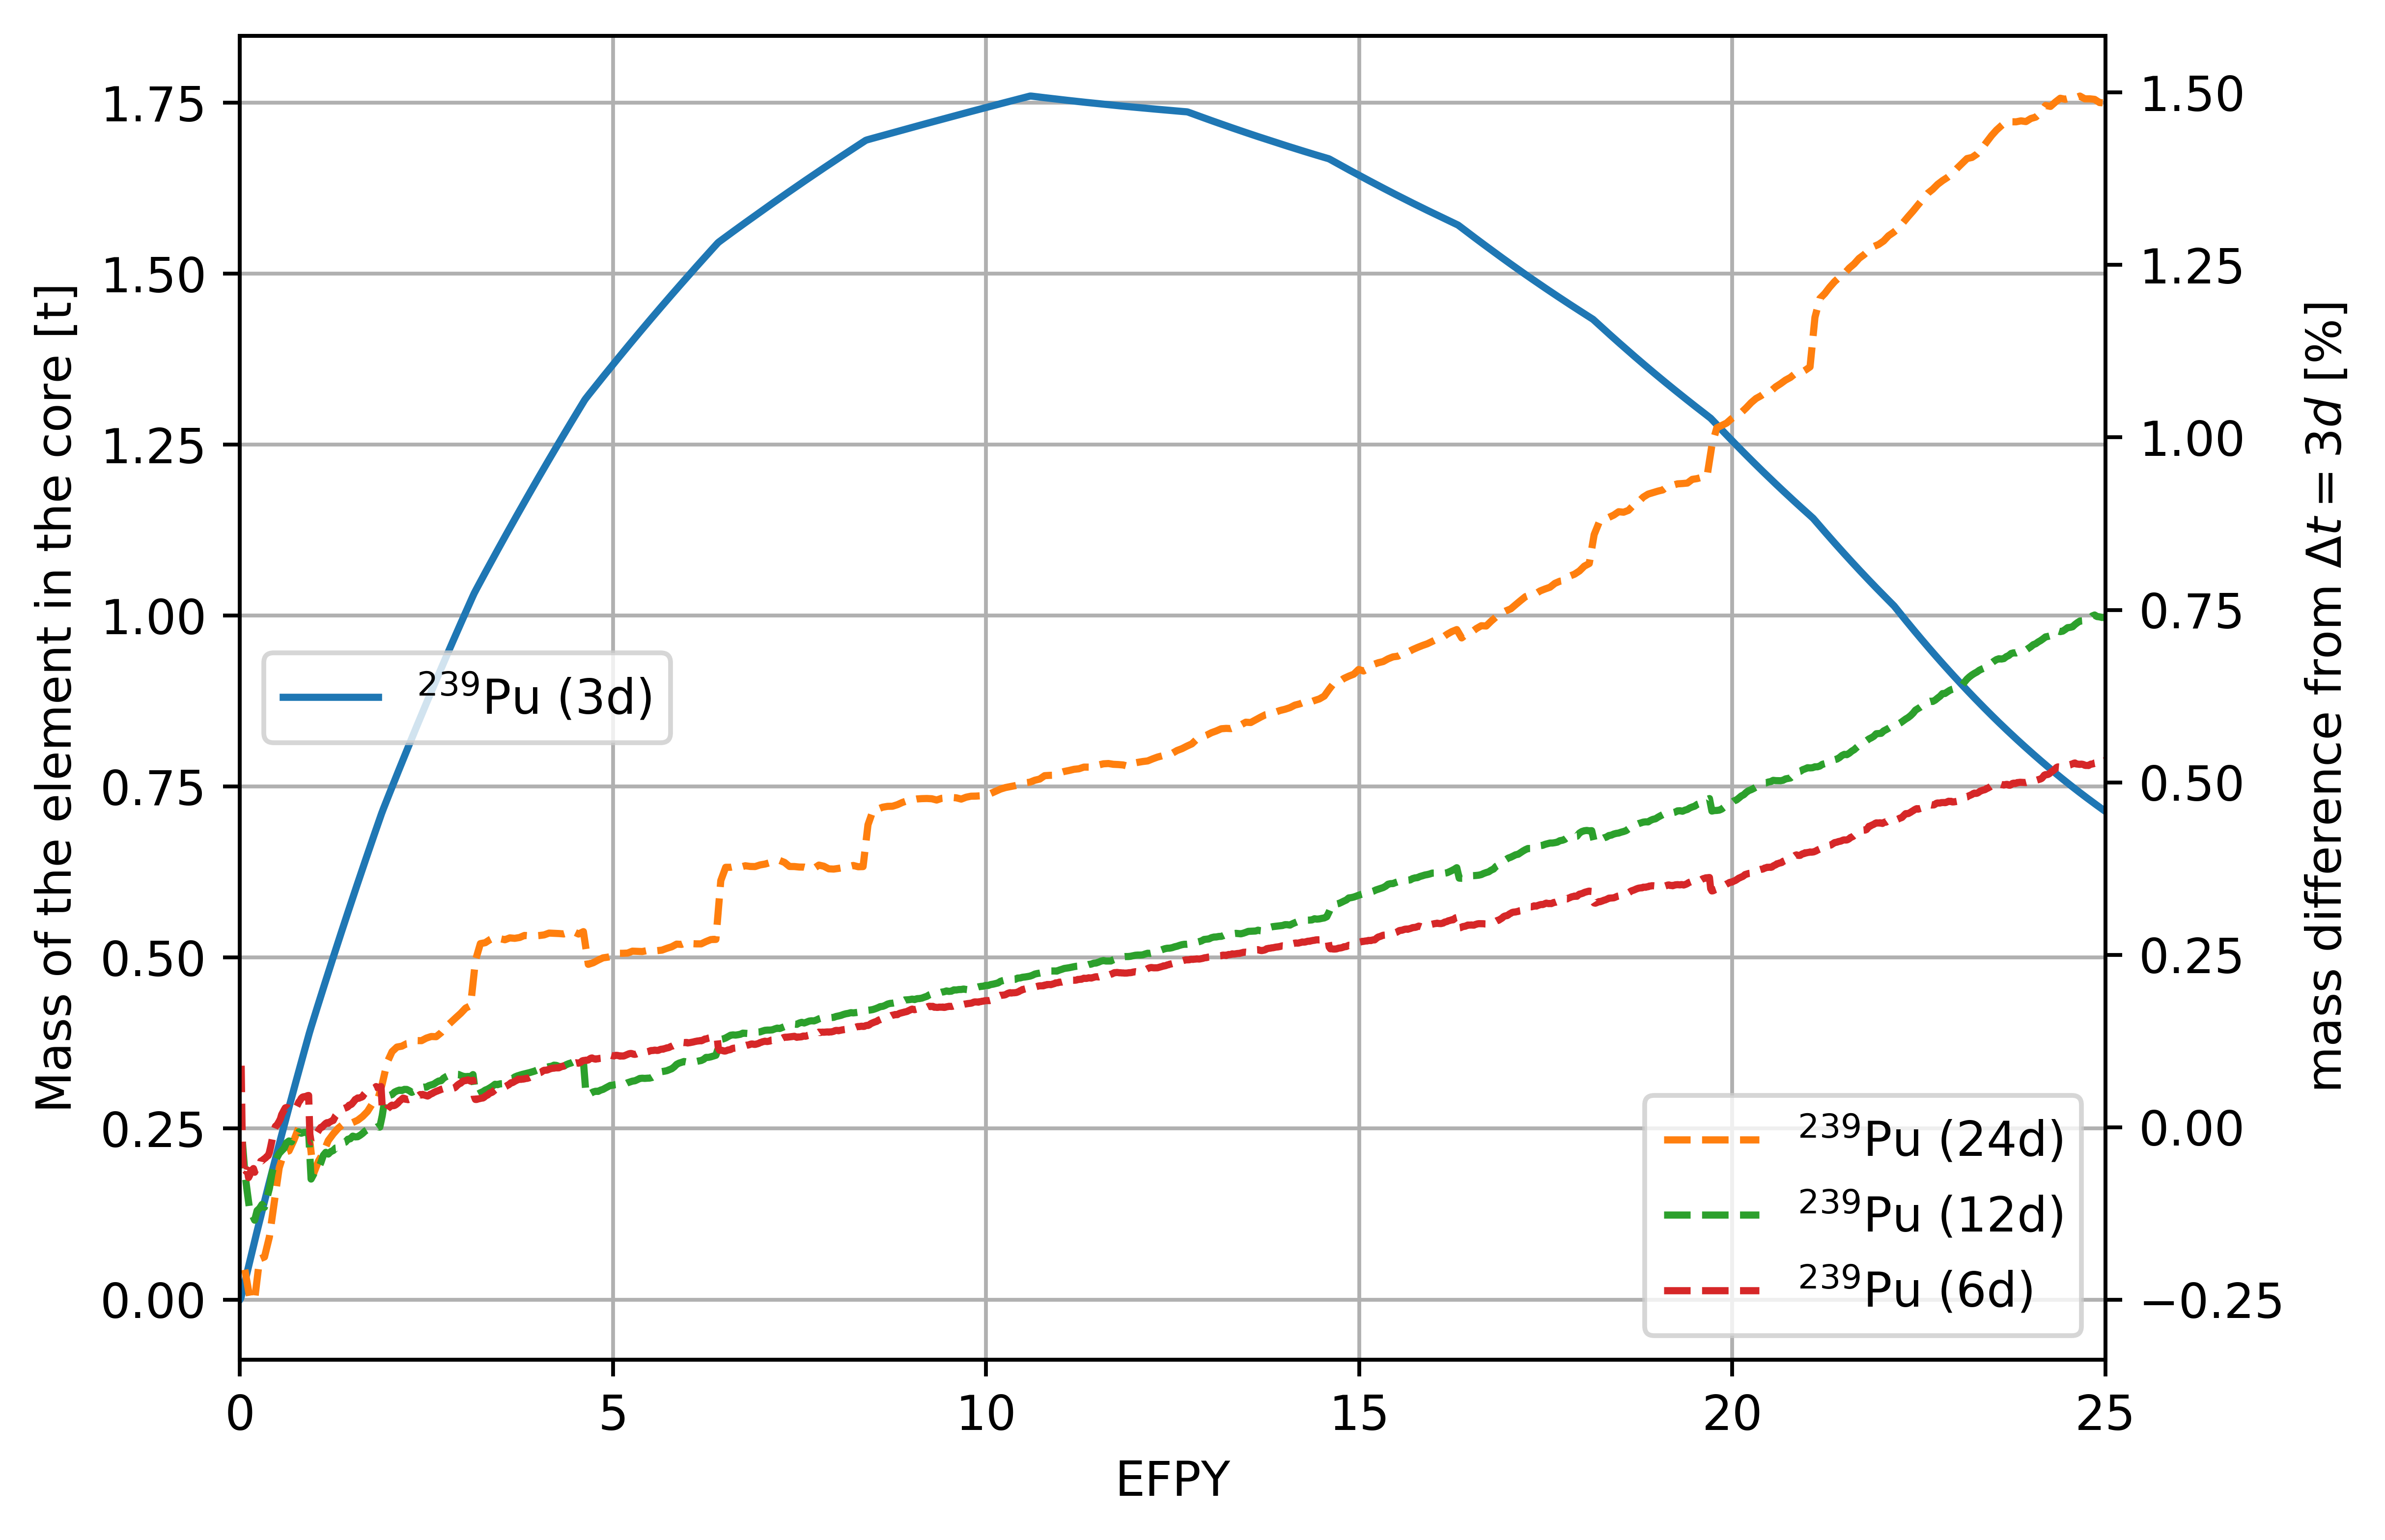
\includegraphics[width=\textwidth]{ch4/pu239_time_refinement.png}
	\caption{SaltProc-calculated $^{239}$Pu content during operation for 
		different depletion time step sizes.}
	\label{fig:timeref-pu239}
\end{figure}
Increasing depletion time interval significantly reduces computational cost 
but also significantly deteriorates the accuracy of depletion calculations. 
Calculations using a depletion time step of 6 days and longer demonstrated a 
significant difference in calculated $k_{eff}$ and depleted mass from those 
using 3-day depletion step. In the current work, 3-day depletion step was 
selected to adequately predict the mass of major heavy isotopes in the fuel 
salt during 25 years of the \gls{TAP} reactor operation.


\subsection{Realistic extraction efficiency case}\label{sec:long-term-real}
This section demonstrate SaltProc v1.0 for lifetime-long depletion simulation 
similar to Section~\ref{sec:ben-valid}, but with realistic, physics-based 
correlation for noble gas removal efficiency. For the demonstration case 
herein efficiency of xenon, krypton, and hydrogen extraction are determined 
using Peebles \emph{et al.} model (Equation~\ref{eq:gas_eff}) discussed 
earlier. Gas-liquid interfacial area per unit volume ($a$) to inform 
equation~\ref{eq:gas_eff} is a function of salt/gas flow rates and diameter of 
the gas bubbles 
\cite{sada_gas-liquid_1987}:
\begin{align}\label{eq:interfacial-area}
& a = \frac{6}{d_b}\frac{Q_{He}}{Q_{He} + Q_{salt}}
\intertext{where}
Q_{salt}&= \mbox{volumetric salt flow rate $[m^3/s]$} \nonumber \\
Q_{He}&= \mbox{volumetric helium flow rate $[m^3/s]$} \nonumber \\
d_b &= \mbox{helium bubble diameter $[m]$.} \nonumber
\end{align}

Additionally, following parameters are selected to inform 
Equation~\ref{eq:gas_eff} for prototypic sparger: (1) salt volumetric flow 
rate throughout sparger $Q_{salt}=2$ $m^3/s$; (2) sparging gas (helium) 
volumetric flow rate $Q_{He}=0.1$ $m^3/s$; (3) helium bubbles diameter 
$d_b=0.508$ $mm$ as advised by ORNL \cite{robertson_conceptual_1971}; (4) 
length of the sparger $L=11$ $m$; (5) sparger diameter $D=0.4$ $m$ (sparger 
cross section $A_C=0.126$ $m^2$).

The liquid phase mass transfer coefficient ($K_L$) selection presents a 
challenge, since published information is currently insufficient to inform 
Equation~\ref{eq:gas_eff}. 
Peebles \emph{et al.} stated that Equation~\ref{eq:gas_eff} is valid for $K_L$
in range from 1 to 100 $ft/hr$ (from 0.0847 to 8.4667 $mm/s$) 
\cite{peebles_removal_1968}. For the demonstration case herein, I performed a
25-year depletion calculations for $K_L$ of 0.0847, 2.1167, and 8.4667 $mm/s$ 
to investigate the effect of noble gas removal efficiency on fuel cycle 
characteristics.

Extraction efficiency is gas-specific because solubility in the salt (Henry's 
law constant) is different for various gases. 
Table~\ref{tab:gas_removal_efficiency} reports dimensionless Henry's law 
constant and corresponding calculated efficiency of noble gas (Xe, Kr, H) 
migration to the helium bubbles ($\epsilon_m$) in the prototypic sparger for 
various mass transfer coefficients ($K_L$).  Total separation efficiency  
(Table~\ref{tab:gas_removal_efficiency}, last 3 columns) refers efficiency of 
extraction target gaseous element after performing helium sparging in the 
sparger following by separation of noble-gas-reach bubbles from the salt in 
the axial-flow centrifugal bubble separator \cite{gabbard_development_1974}. 


%%%%%%%%%%%%%%%%%%%%%%%%%%%%%%%%%%%%%%%%
\begin{table}[htp!]
	\fontsize{9}{11}\selectfont
	\centering
	\caption{The noble gas extraction efficiency at working temperature 
		T=627$^{\circ}$C calculated using Peebles \emph{et al.} model 
		(Equation~\ref{eq:gas_eff}) assuming salt volumetric flow 
		rate $Q_{salt}=2$ $m^3/s$, helium volumetric flow rate $Q_{He}=0.1$ 
		$m^3/s$, helium bubbles diameter $d_b=0.508$ $mm$, and volume of the 
		sparger $V=1.4$ $m^3$. The liquid phase mass transfer coefficient 
		($K_L$) is varied in validity range $[0.0847,8.4667]$ $mm/s$ 
		\cite{peebles_removal_1968}.}
	\begin{tabularx}{\textwidth}{L X R R R R R R}
		\hline 
		\textbf{Element}&\textbf{Henry's}& 
		\multicolumn{6}{c}{\textbf{Efficiency of}} \\
		& \textbf{law}& \multicolumn{3}{c}{\textbf{migration to He bubbles 
		($\epsilon_m$)}}& \multicolumn{3}{c}{\textbf{total separation 
		($\epsilon$)$^{\star}$}} \\
		&\textbf{constant} & \multicolumn{3}{c}{\textbf{for $K_L$ [mm/s]}} 
		&\multicolumn{3}{c}{\textbf{for $K_L$ [mm/s]}}\\
		&\textbf{($K_H$)$[-]$} & 8.4667&2.1167&0.0847&8.4667&2.1167&0.0847\\
		\hline
		Xe &5.7E-5 \cite{blander_solubility_1959}&0.9630&0.5639&0.0327&	
		0.9149&0.5357&0.0310\\
		Kr &2.8E-4 \cite{blander_solubility_1959}&0.9595&0.5630&0.0327& 
		0.9115&0.5349&0.0310\\
		H  &3.9E-3 \cite{tomkins_gases_2016}&0.9066&0.5499&0.0326&
		0.8613&0.5224&0.0309\\	
		\hline
	\end{tabularx}
	\begin{tablenotes}
		\footnotesize
		\item$^{\star}$With axial-flow centrifugal bubble separator by 
		Gabbard \emph{et al.} which allows the bubble separation efficiency 
		$\epsilon_{es}$=0.95 \cite{gabbard_development_1974}. Thus, total 
		gas removal efficiency ($\epsilon$) can be calculated as follows: 
		$\epsilon=\epsilon_m\times \epsilon_{es}$.
	\end{tablenotes}
	\label{tab:gas_removal_efficiency}
	\vspace{-0.9em}
\end{table}
%%%%%%%%%%%%%%%%%%%%%%%%%%%%%%%%%%%%%%%%%%%%%%%%%%%%%%%%%%%%%%%%%%%%%%%%%%%%%%%


\subsubsection{Effective multiplication factor dynamics}
Figure~\ref{fig:keff-eps-var} and \ref{fig:keff-eps-var-zoom} demonstrate the 
effective multiplication factor dynamics ($k_{eff}$) during 25 years of 
operation obtained using SaltProc v1.0 and Serpent. SaltProc calculated 
$k_{eff}$ after removing fission products and feeding 5\% \gls{LEU} at the end 
of each depletion step (3 days as was determined in 
Section~\ref{sec:time-refinement}). Notably, the core went subcritical during 
first cycle (startup moderator rod configuration) after 330 and 318 days for 
$K_L=8.4667$ and 0.0847 $mm/s$, respectively. 

Lower mass transfer coefficient worsen efficiency of neutron poison removal 
from the \gls{TAP} core which is shortening interval between shutdowns for 
moderator rod updates. Additionally, the presents of unremoved poison in the 
core suppresses the effective multiplication factor after moderator 
reconfiguration ($\approx500$ $pcm$ lower for $K_L=0.0847$ $mm/s$ case than 
for $K_L=8.4667$ $mm/s$ at the \gls{BOL} and $\approx1100$ $pcm$ at the 
\gls{EOL}). Overall, noble gas removal provides with significant neutronics 
benefit (less neutrons are being lost in strong absorbers such as $^{135}$Xe), 
better fuel utilization, and enables longer time between reconfiguring the 
moderator rods.
\begin{figure}[htp!] % replace 't' with 'b' to 
	\centering
	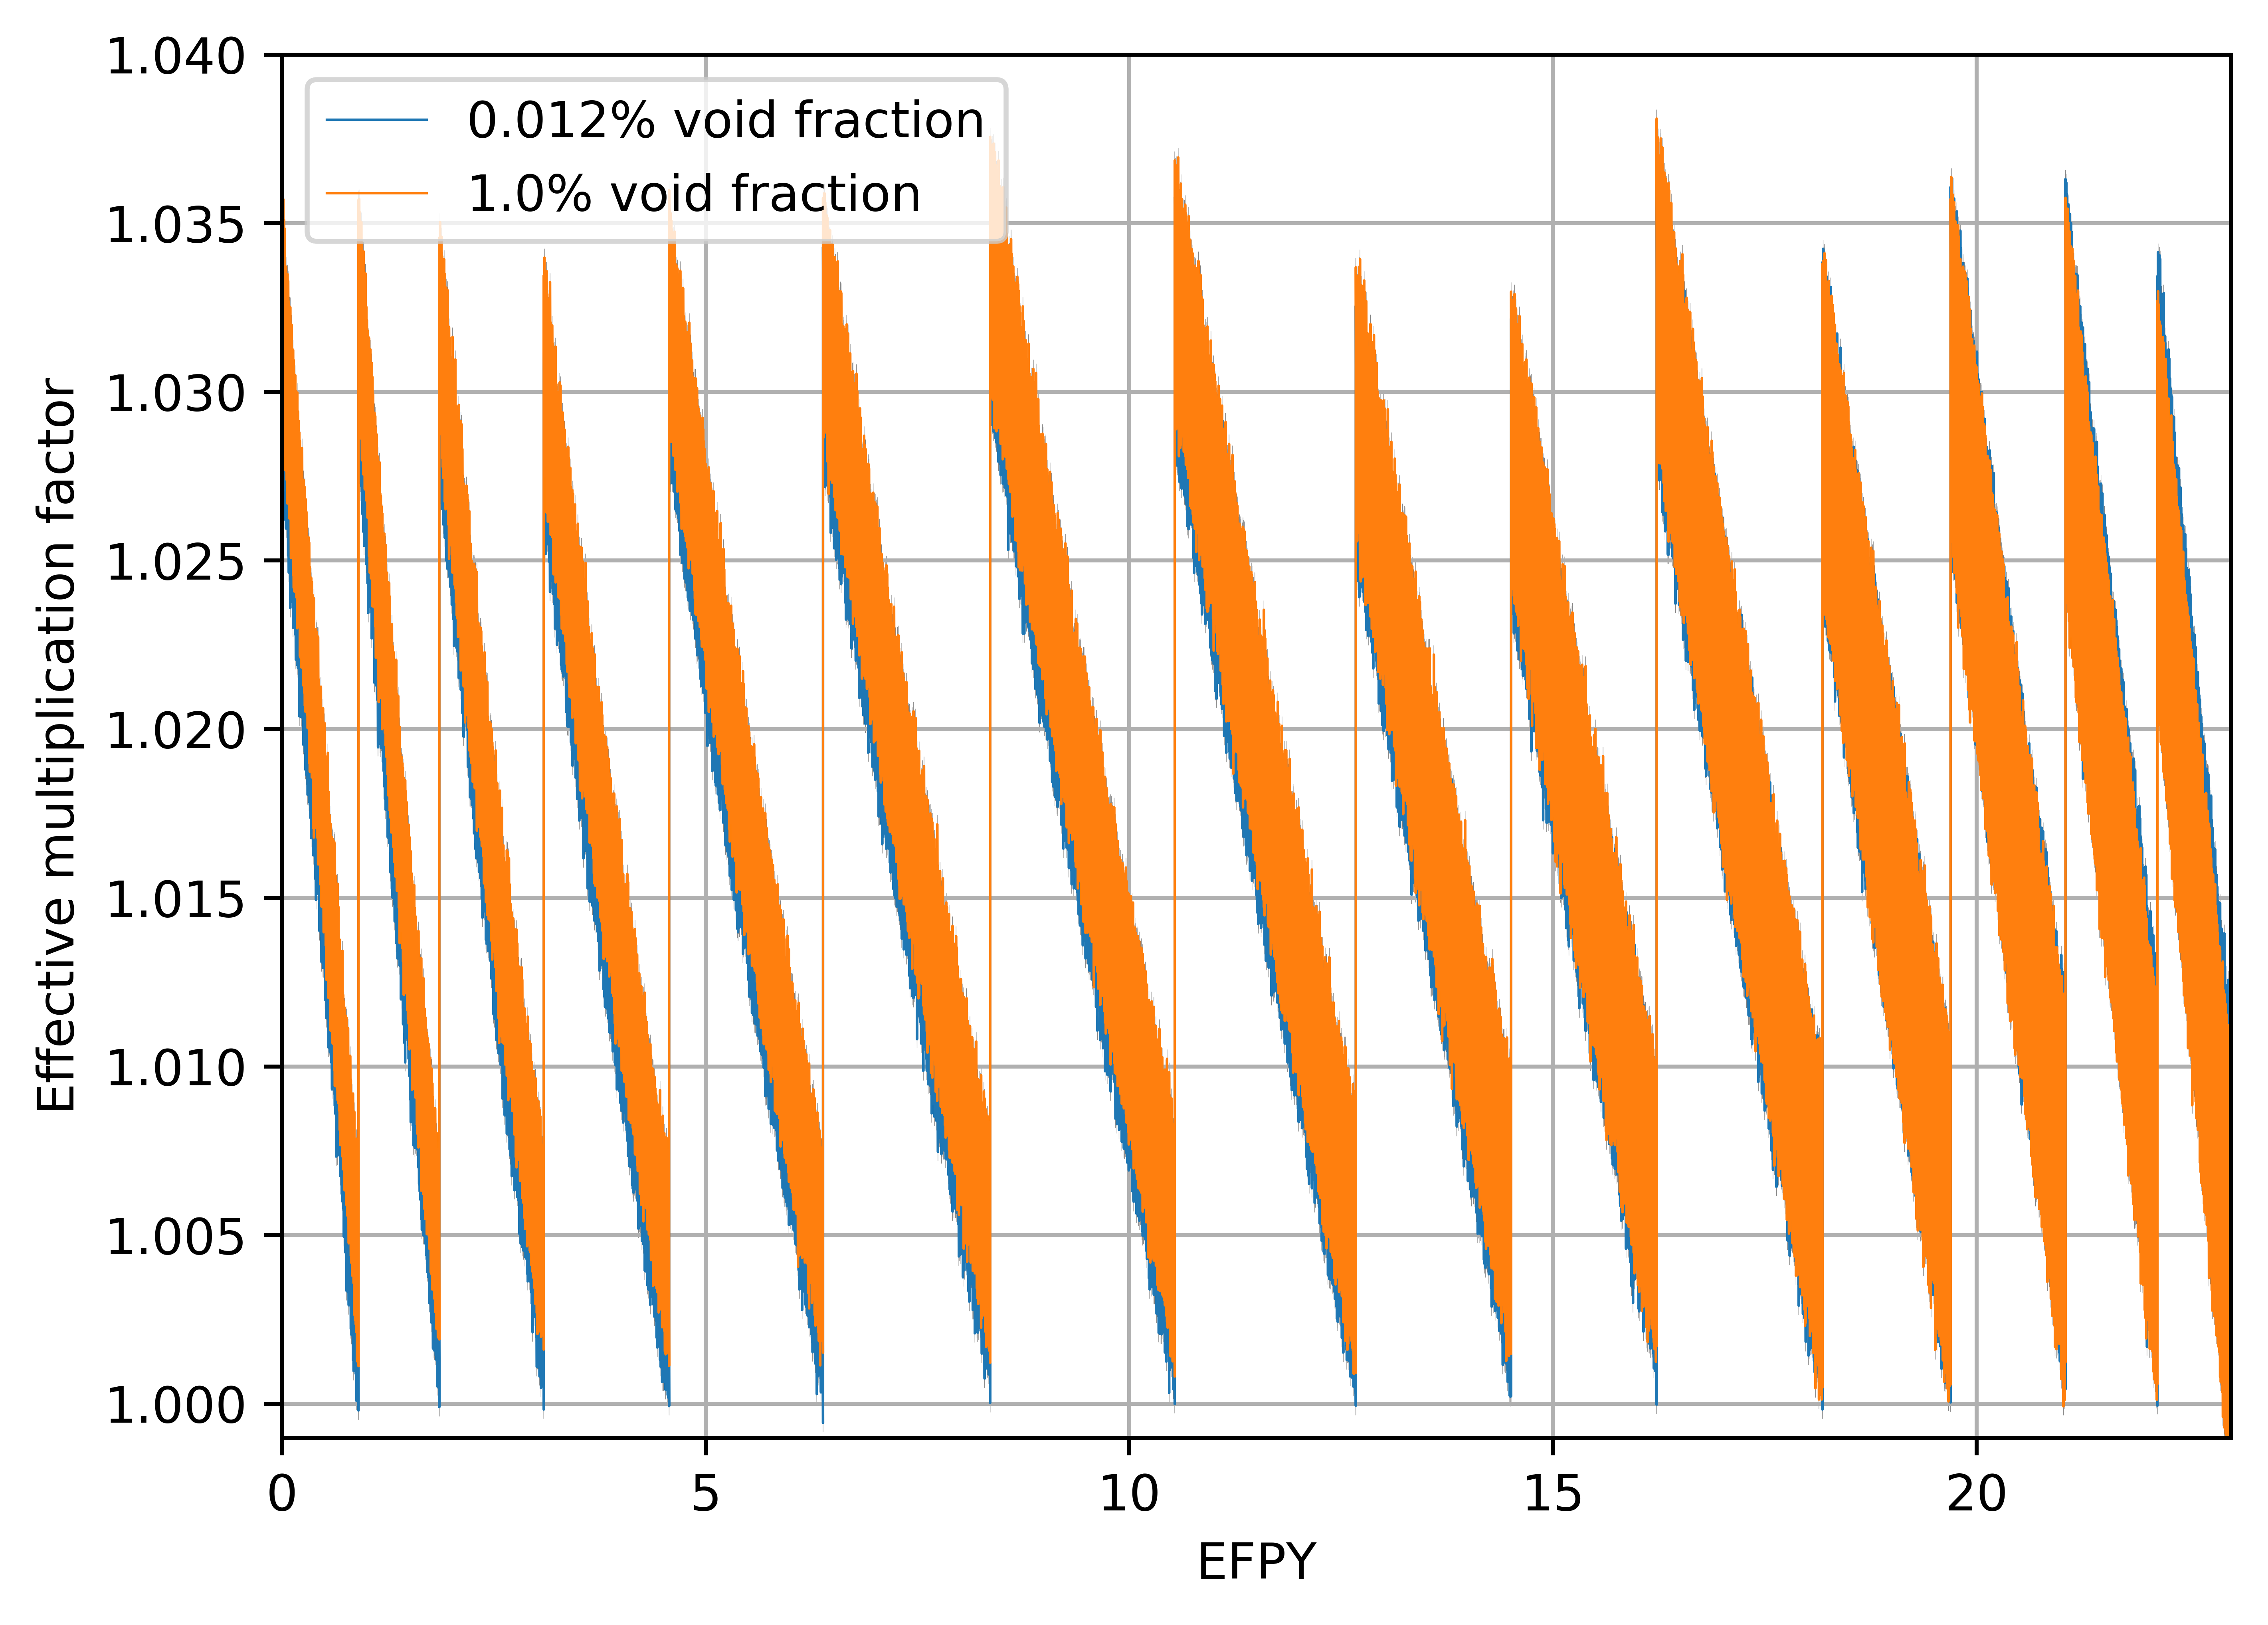
\includegraphics[width=\textwidth]{ch4/eps/keff.png}
	\caption{Effective multiplication factor dynamics for full-core \gls{TAP} 
		core model during 25 years of operation for the case with realistic 
		removal efficiency of fission product and various mass transfer 
		coefficients ($K_L$). Confidence interval $\sigma=28$ $pcm$ is shaded.}
	\label{fig:keff-eps-var}
\end{figure}

\begin{figure}[htbp!] % replace 't' with 'b' to 
	\centering
	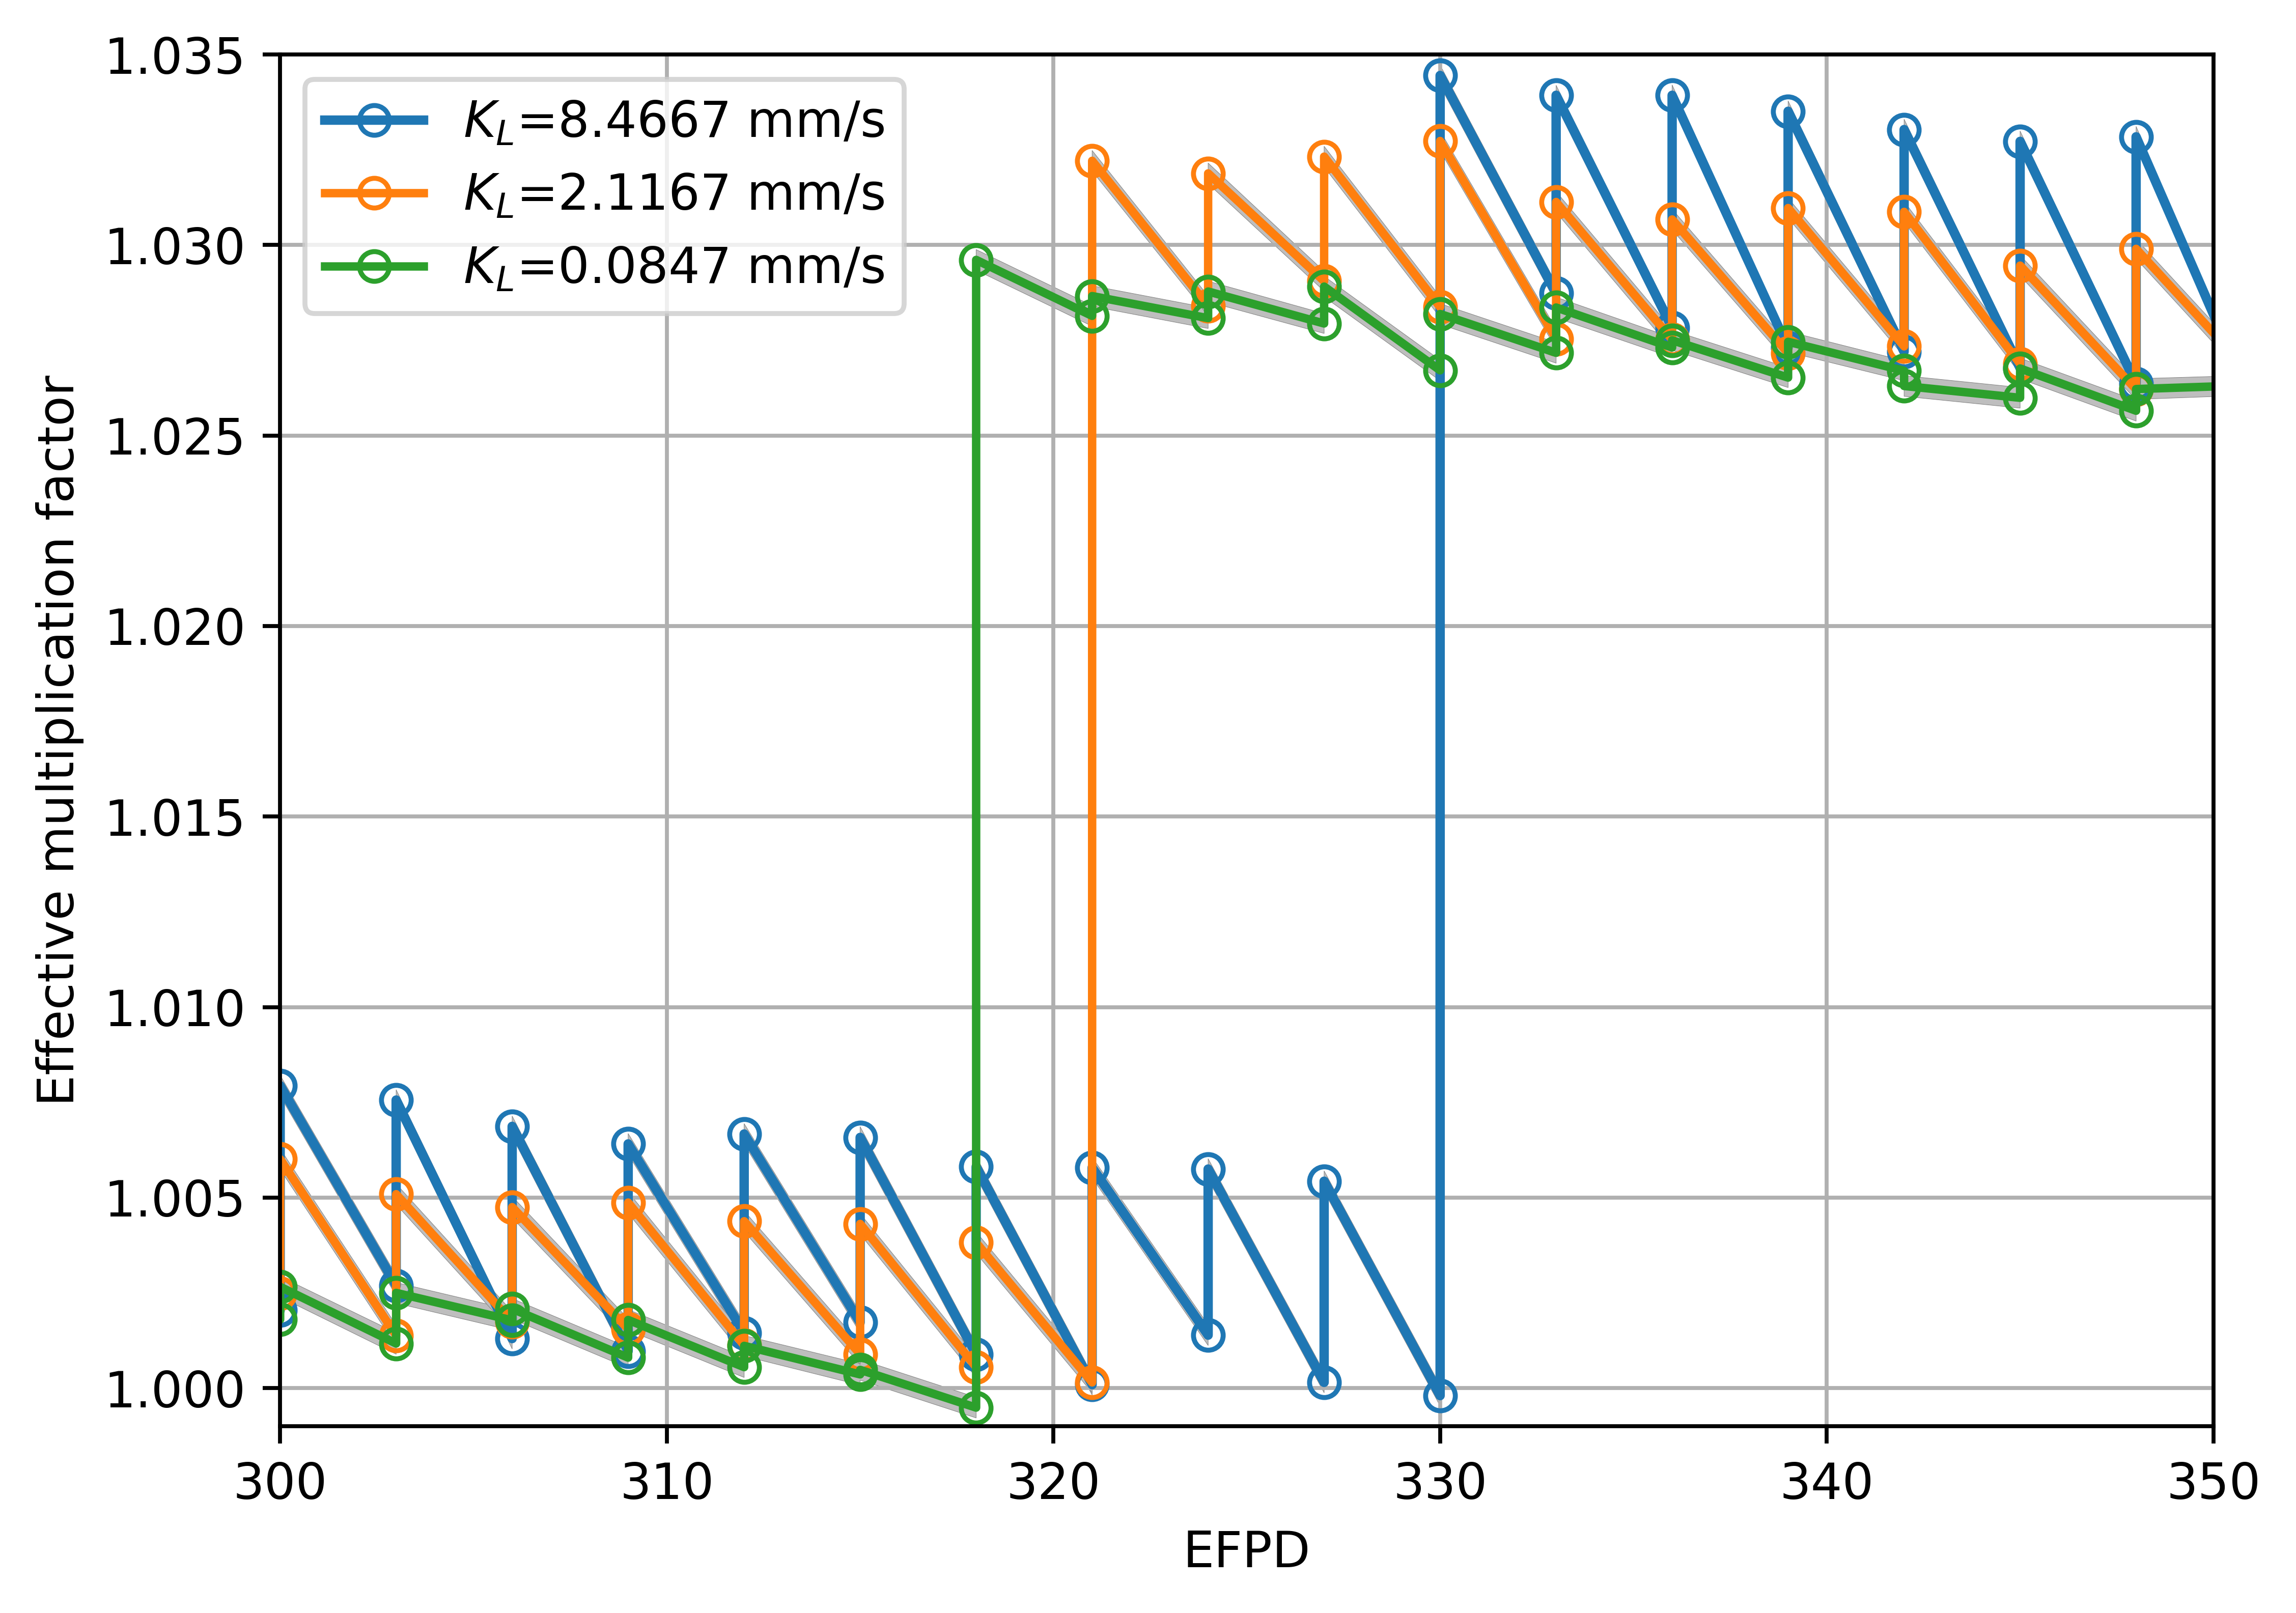
\includegraphics[width=0.93\textwidth]{ch4/eps/keff_zoomed_1.png}\\
	\vspace{-8mm}
		\hspace{+1mm}
	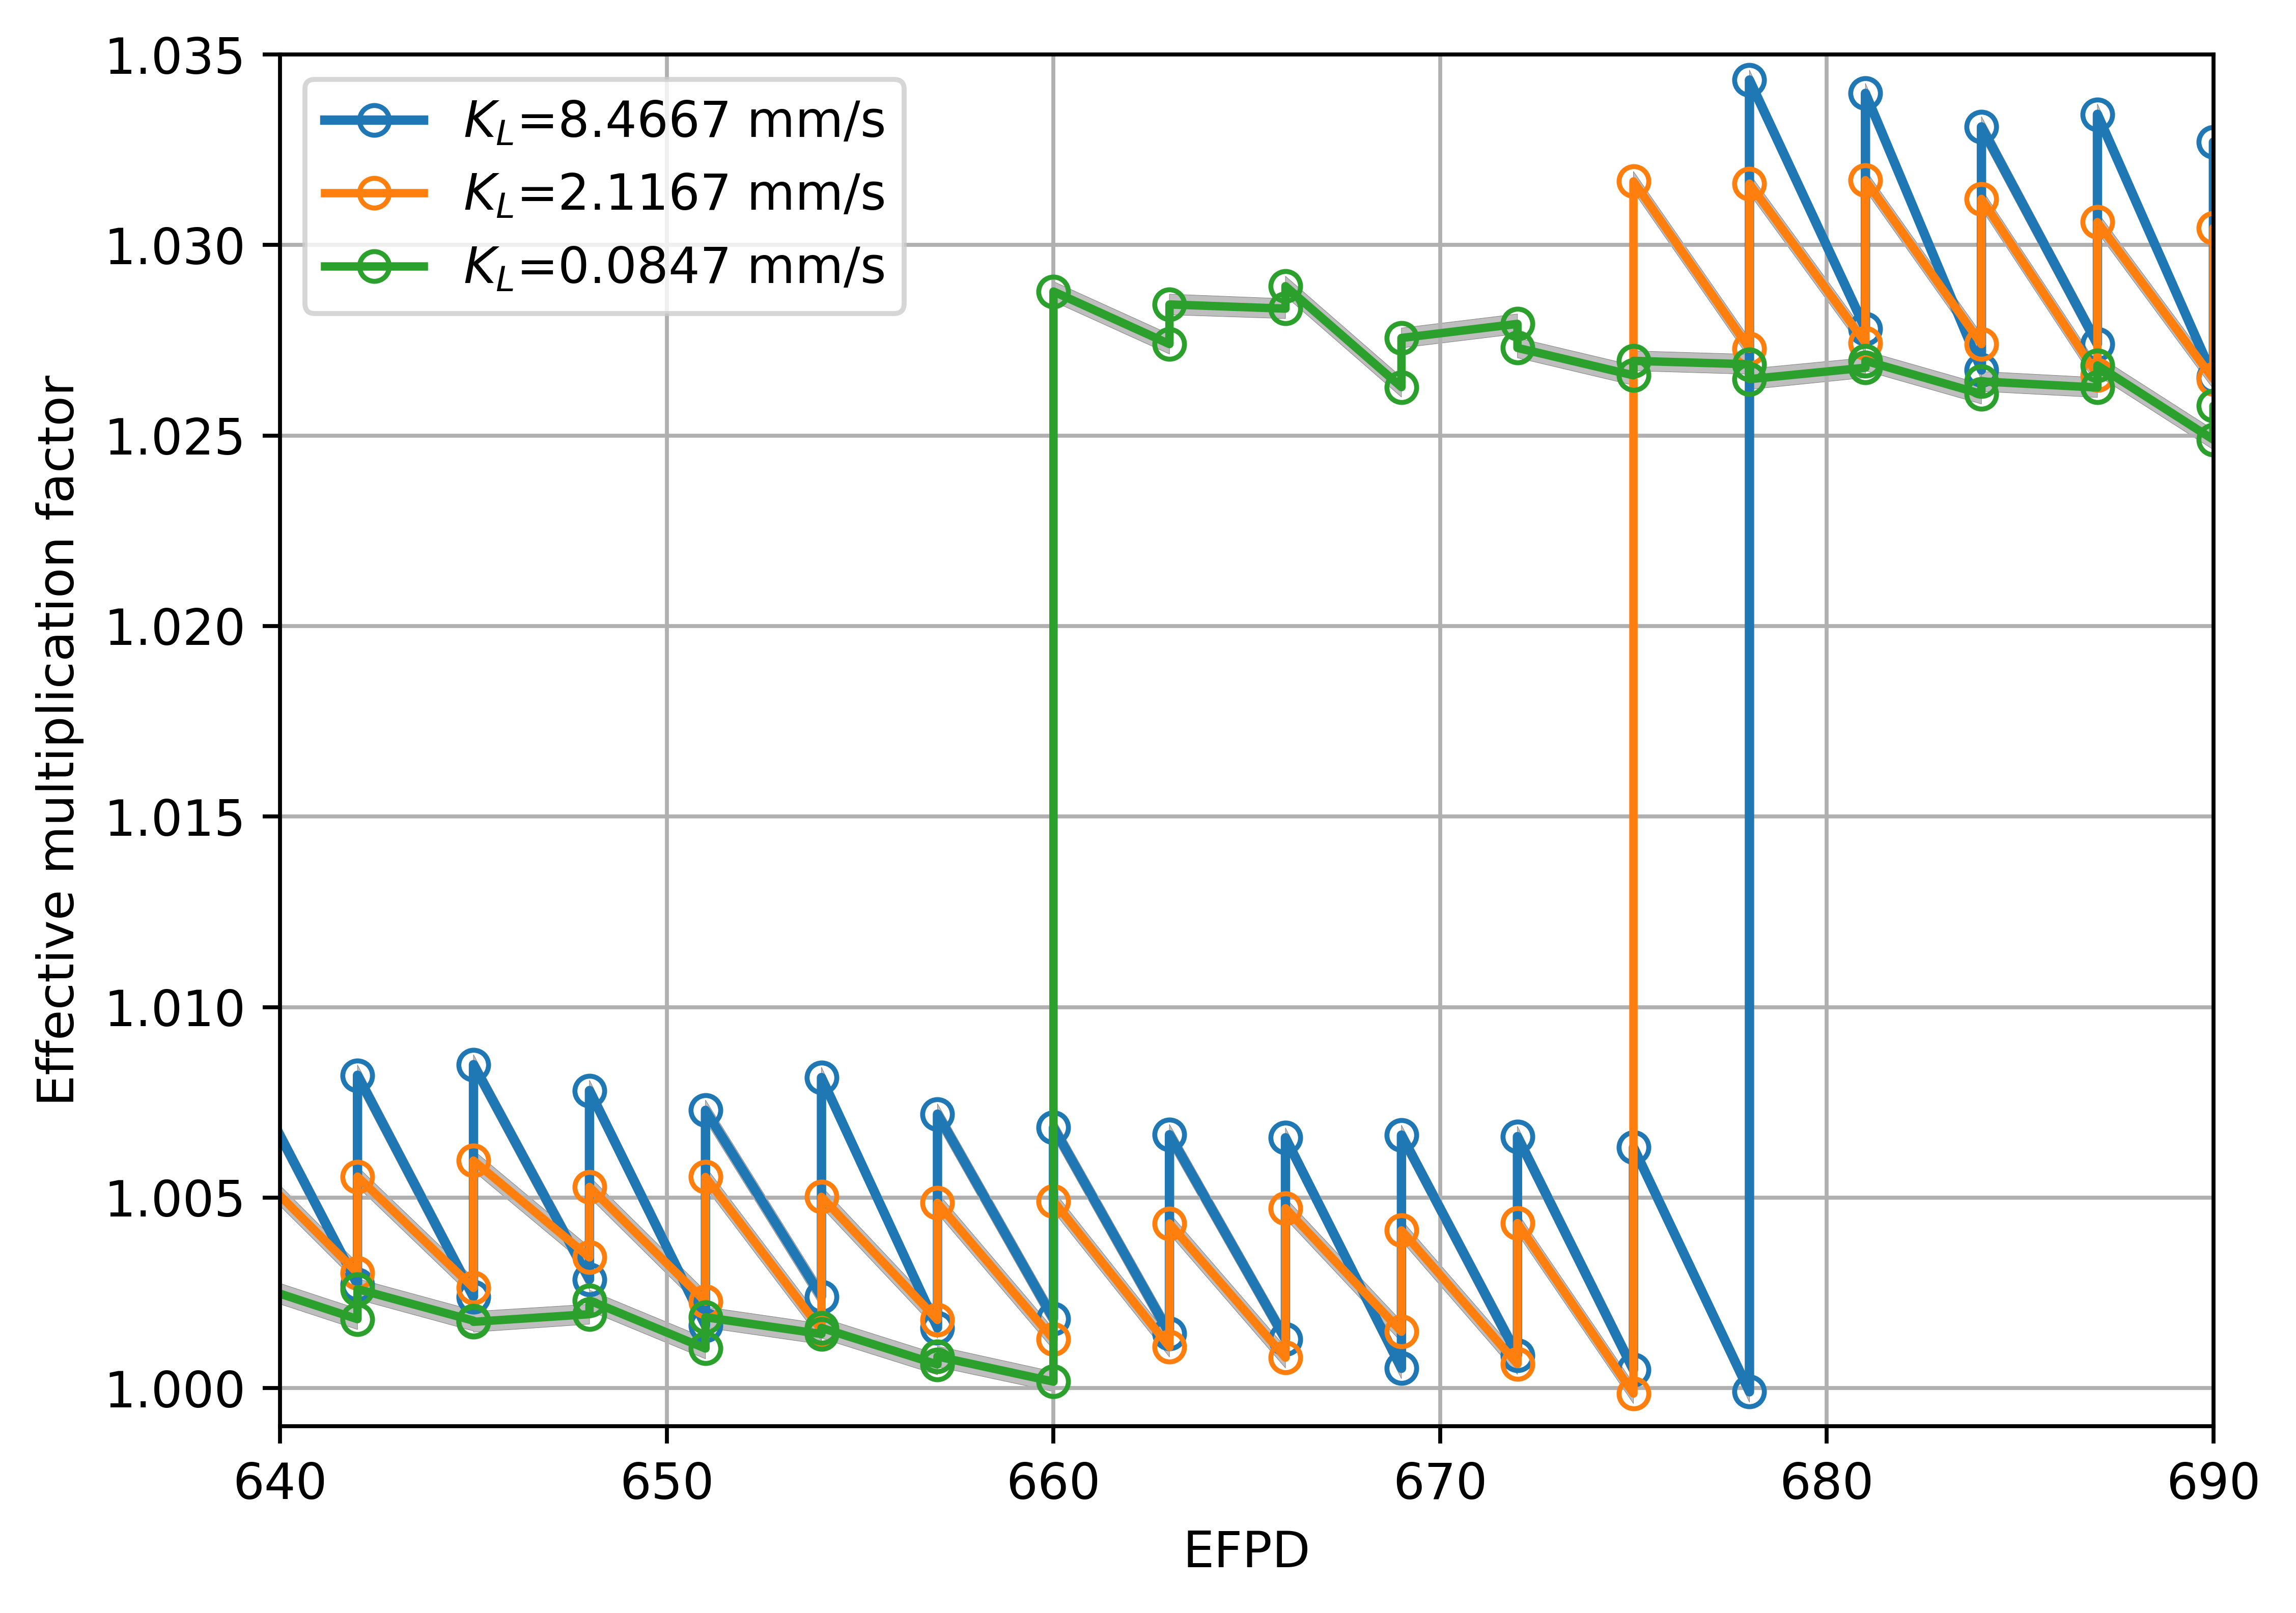
\includegraphics[width=0.93\textwidth]{ch4/eps/keff_zoomed_2.png}
	\vspace{-3mm}
	\caption{Zoomed effective multiplication factor dynamics during switching
	from Cycle \#1 (startup geometry configuration, 347 moderator rods, 
	\gls{SVF}=0.91720353) to Cycle \#2 (\gls{SVF}=0.88694) (upper panel) and
	from Cycle \#2 to  Cycle \#3 (\gls{SVF}=0.881092) 
	(lower panel) for various mass transfer coefficients ($K_L$). 
	Confidence interval $\sigma=28$ $pcm$ is shaded.}
	\label{fig:keff-eps-var-zoom}
\end{figure}

\subsubsection{Neutron spectrum}
Figure~\ref{fig:spectrum-eps-var} shows the normalized neutron flux spectrum 
for the full-core TAP core model
in the energy range from 10$^{-9}$ to 15 MeV. 
The neutron energy spectrum at the \gls{EOL} is
significantly harder than at 
the \gls{BOL} due to moderator-to-fuel ratio growth during reactor operation 
caused by periodic moderator rods reconfiguration. The \gls{TAP} reactor 
spectrum is significantly harder
than in a typical \gls{LWR} and is in a good 
agreement with the \gls{TAP} neutroncs white paper 
\cite{transatomic_power_corporation_neutronics_2016} and ORNL 
reports \cite{betzler_assessment_2017-1, betzler_two-dimensional_2017}.
The 
liquid phase mass transfer coefficient ($K_L$) and, consequently, noble gas 
removal efficiency has negligible effect on the spectrum in the fast range 
(between 10$^{-2}$ and 10 MeV) at the \gls{EOL}. 
\begin{figure}[htp!] % replace 't' with 'b' to 
	\centering
	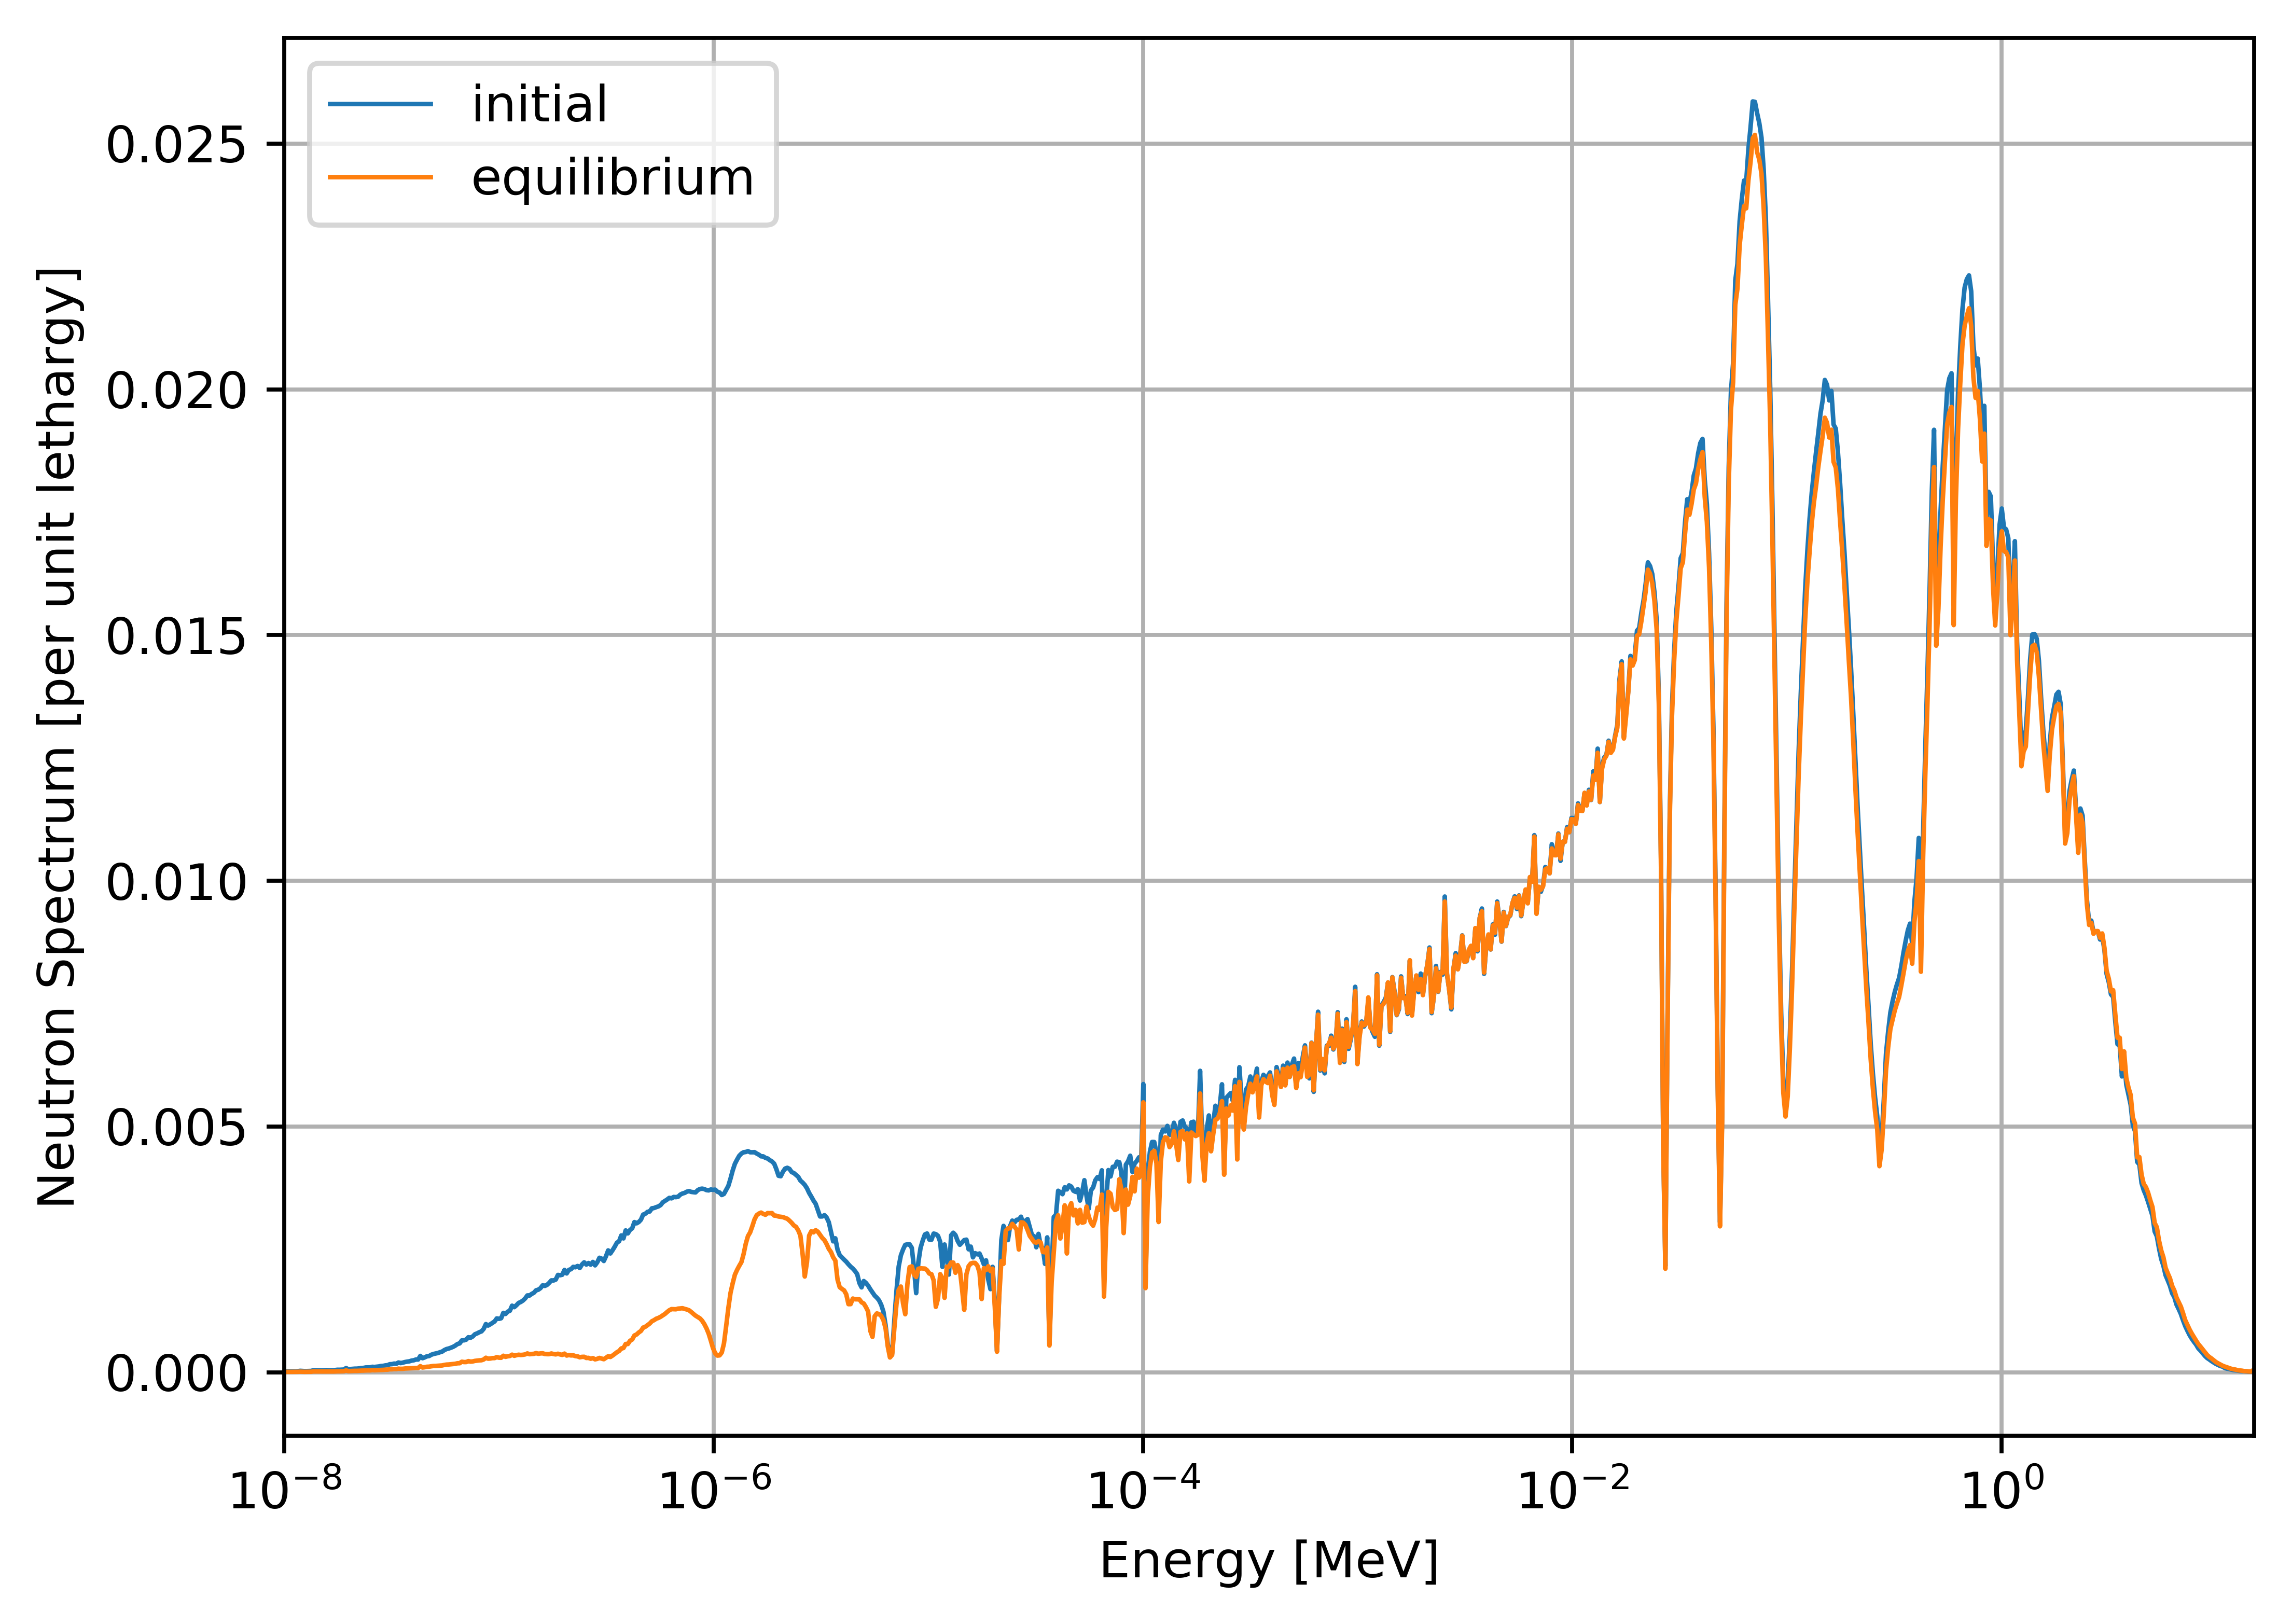
\includegraphics[width=0.7\textwidth]{ch4/eps/spectrum.png}
		\vspace{-3mm}
	\caption{The neutron flux energy spectrum normalized by unit lethargy at 
		the \gls{BOL} and \gls{EOL}	for the case with realistic removal 
		efficiency of fission product and various mass transfer coefficients 
		($K_L$).}
	\label{fig:spectrum-eps-var}
\end{figure}

However, Figure~\ref{fig:spectrum-th-eps-var} demonstrates notable difference 
in thermal range of the spectrum due to huge $^{135}$Xe absorption 
cross section in thermal energy range ($\sigma_{a,^{135}Xe}=2.6\times10^6$ 
b). Figure~\ref{fig:xe135-eps-var-zoomes} shows that $^{135}$Xe mass in the 
core at the \gls{EOL} for the case with low efficiency of noble gas removal 
($K_L=0.0847$ $mm/s$) is significantly larger than for the case with high 
removal efficiency ($K_L=8.4667$ $mm/s$) which leads to higher neutron loss 
due to absorption in xenon.
\begin{figure}[htp!] % replace 't' with 'b' to 
	\centering
	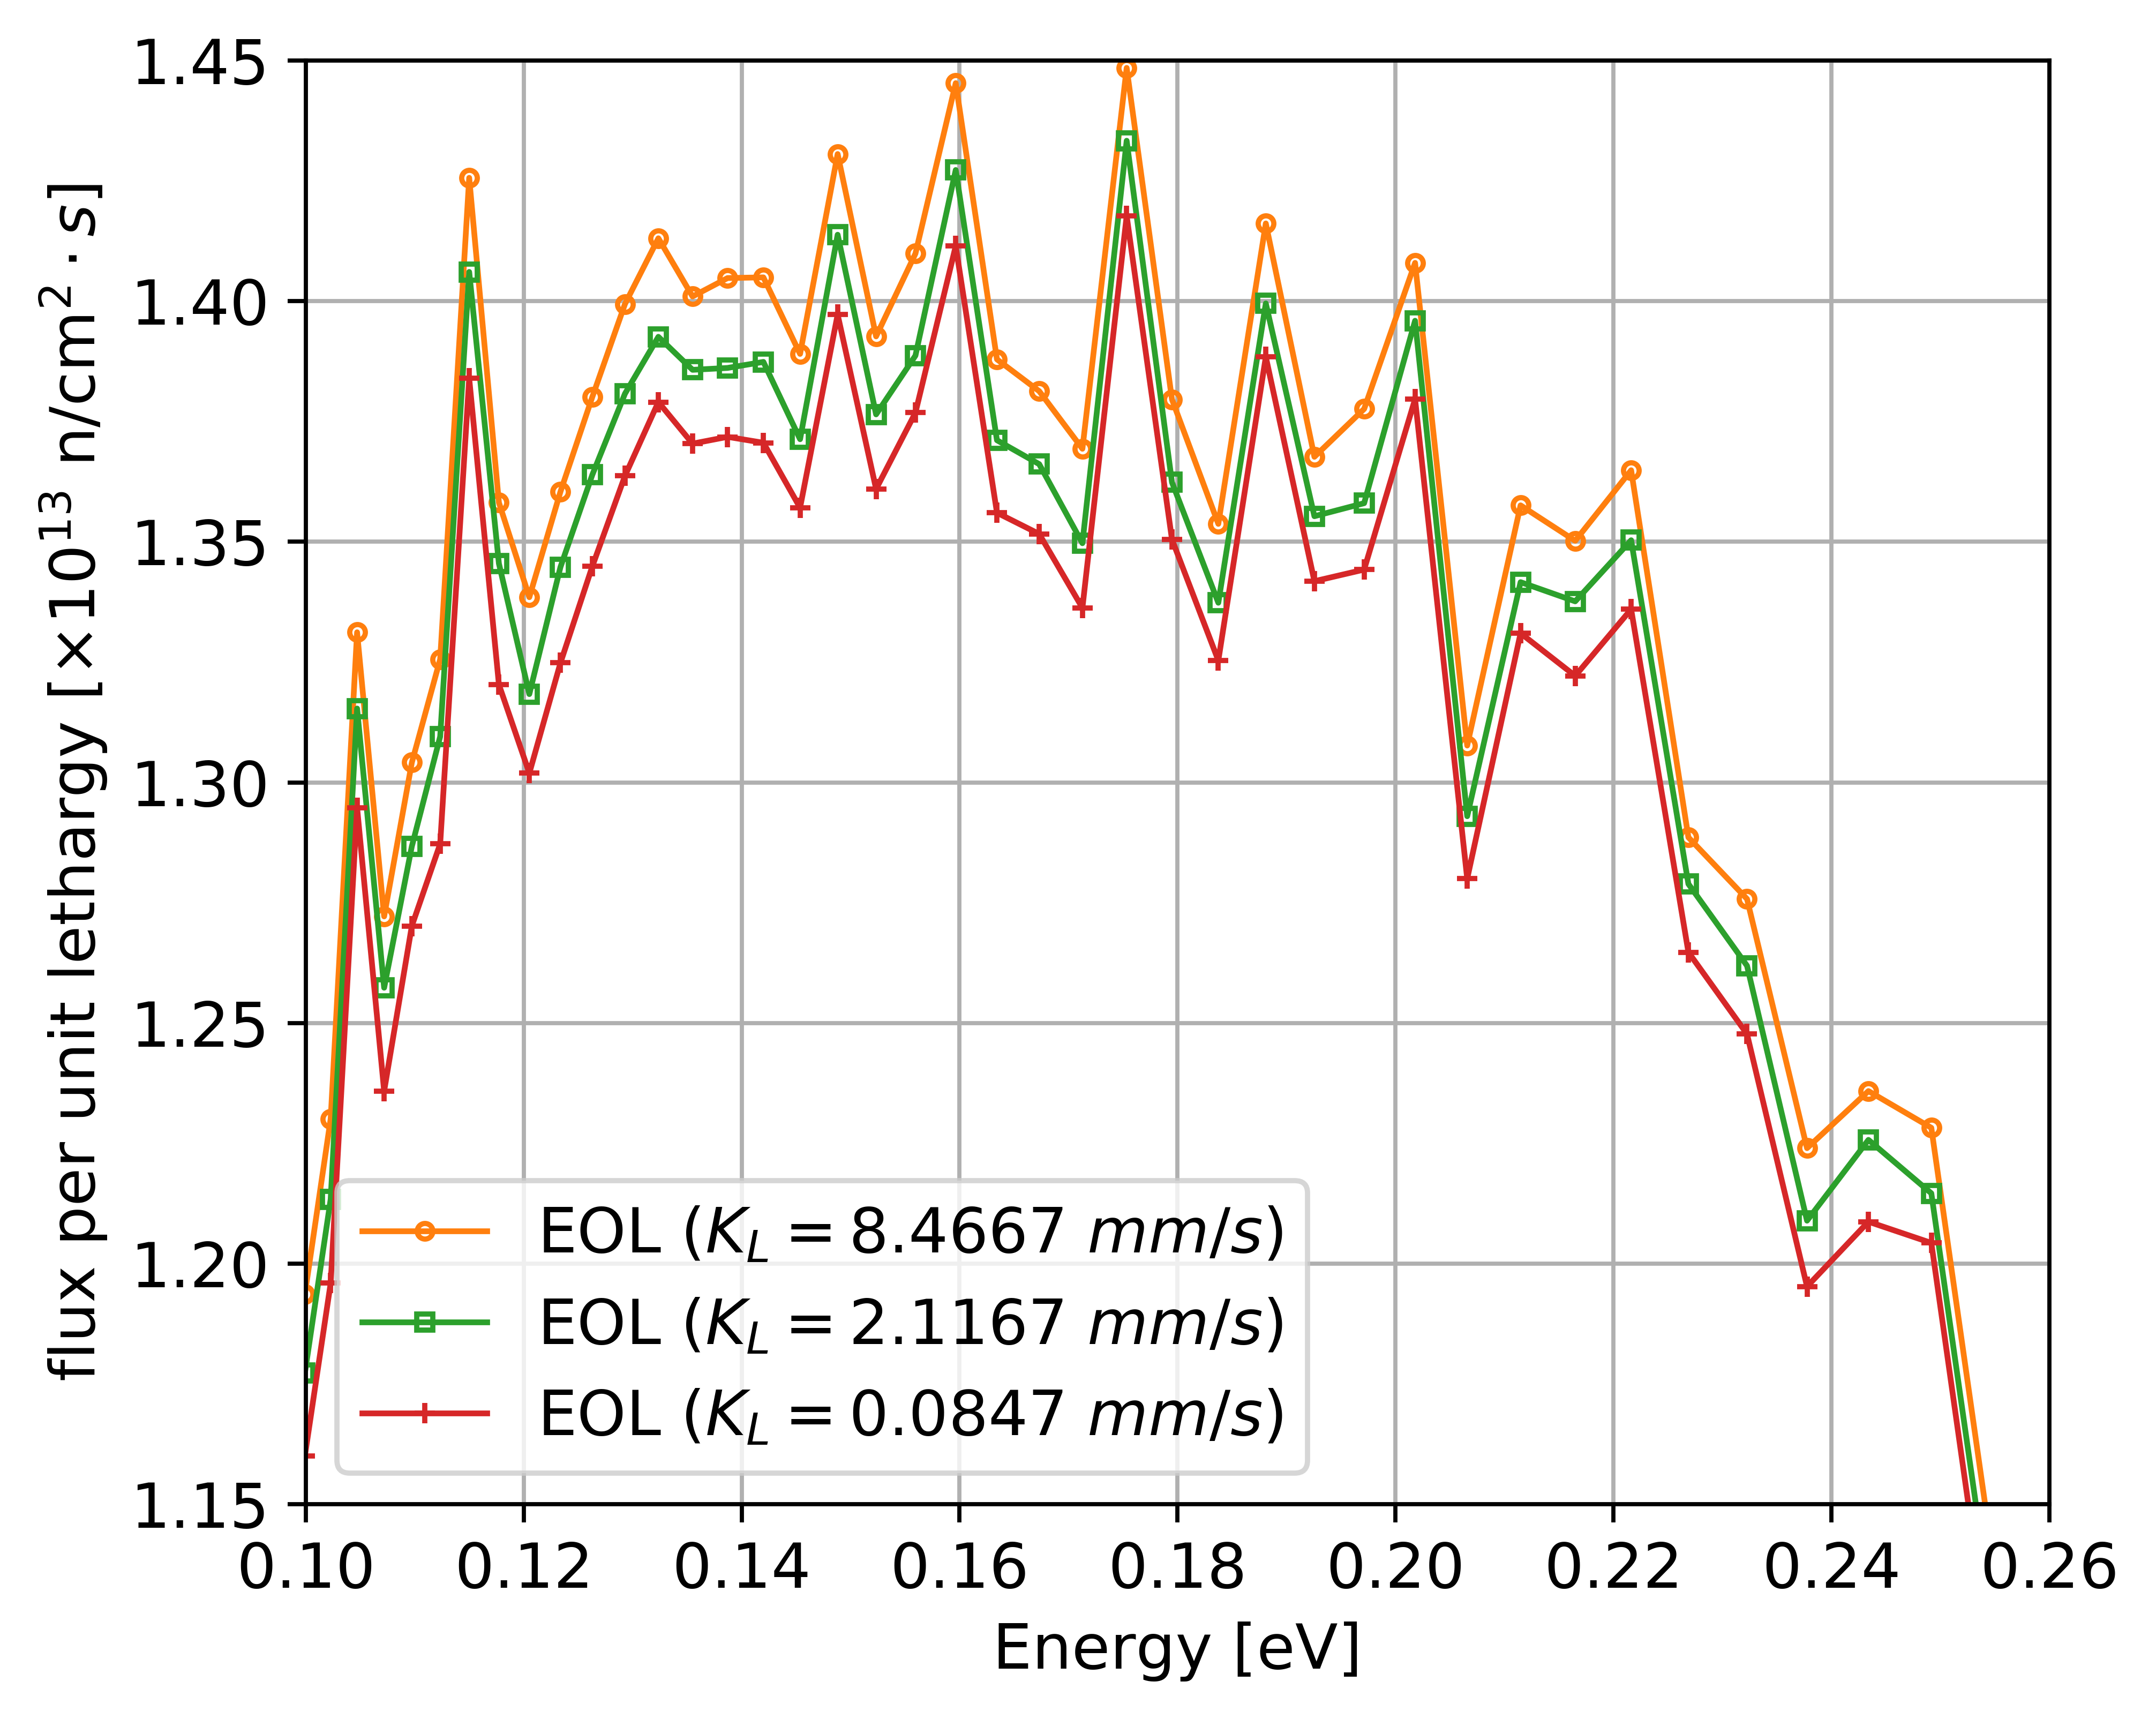
\includegraphics[width=0.7\textwidth]{ch4/eps/spectrum_th_zoomed.png}
			\vspace{-3mm}
	\caption{The neutron flux energy spectrum normalized by unit lethargy  
		\gls{EOL} zoomed in the thermal energy range.}
	\label{fig:spectrum-th-eps-var}
\end{figure}


\subsubsection{Fuel salt isotopic composition evolution}
The time-dependent isotopic compositions obtained with different noble gas 
extraction efficiencies behave very similarly. For $^{235}$U, the difference 
between $K_L=8.4667$ $mm/s$ (e.g., 91.5\% of $^{135}$Xe is removed) and 
$K_L=0.0847$ $mm/s$ (e.g., 3.1\% of $^{135}$Xe is removed) is within 0.2\% for 
the first 14 years and rises rapidly to 1.15\% over the remaining 10 years  
(Figure~\ref{fig:u235-eps-var}). The simulations with mass transfer  
coefficient ($K_L$) smaller than $8.4467$ $mm/s$ maintain a larger quantity of 
$^{235}$U during the operation because more neutrons are being parasitically 
absorbed by the noble gas which leads to slightly smaller fission rate. The 
relative mass difference for $^{238}$U is small 
(Figure~\ref{fig:u238-eps-var}), but absolute difference is approximately 50 
kg at the \gls{EOL}, with the $K_L=0.0847$ $mm/s$ simulation maintaining the 
lower quantity.
\begin{figure}[hbp!] % replace 't' with 'b' to 
	\centering
	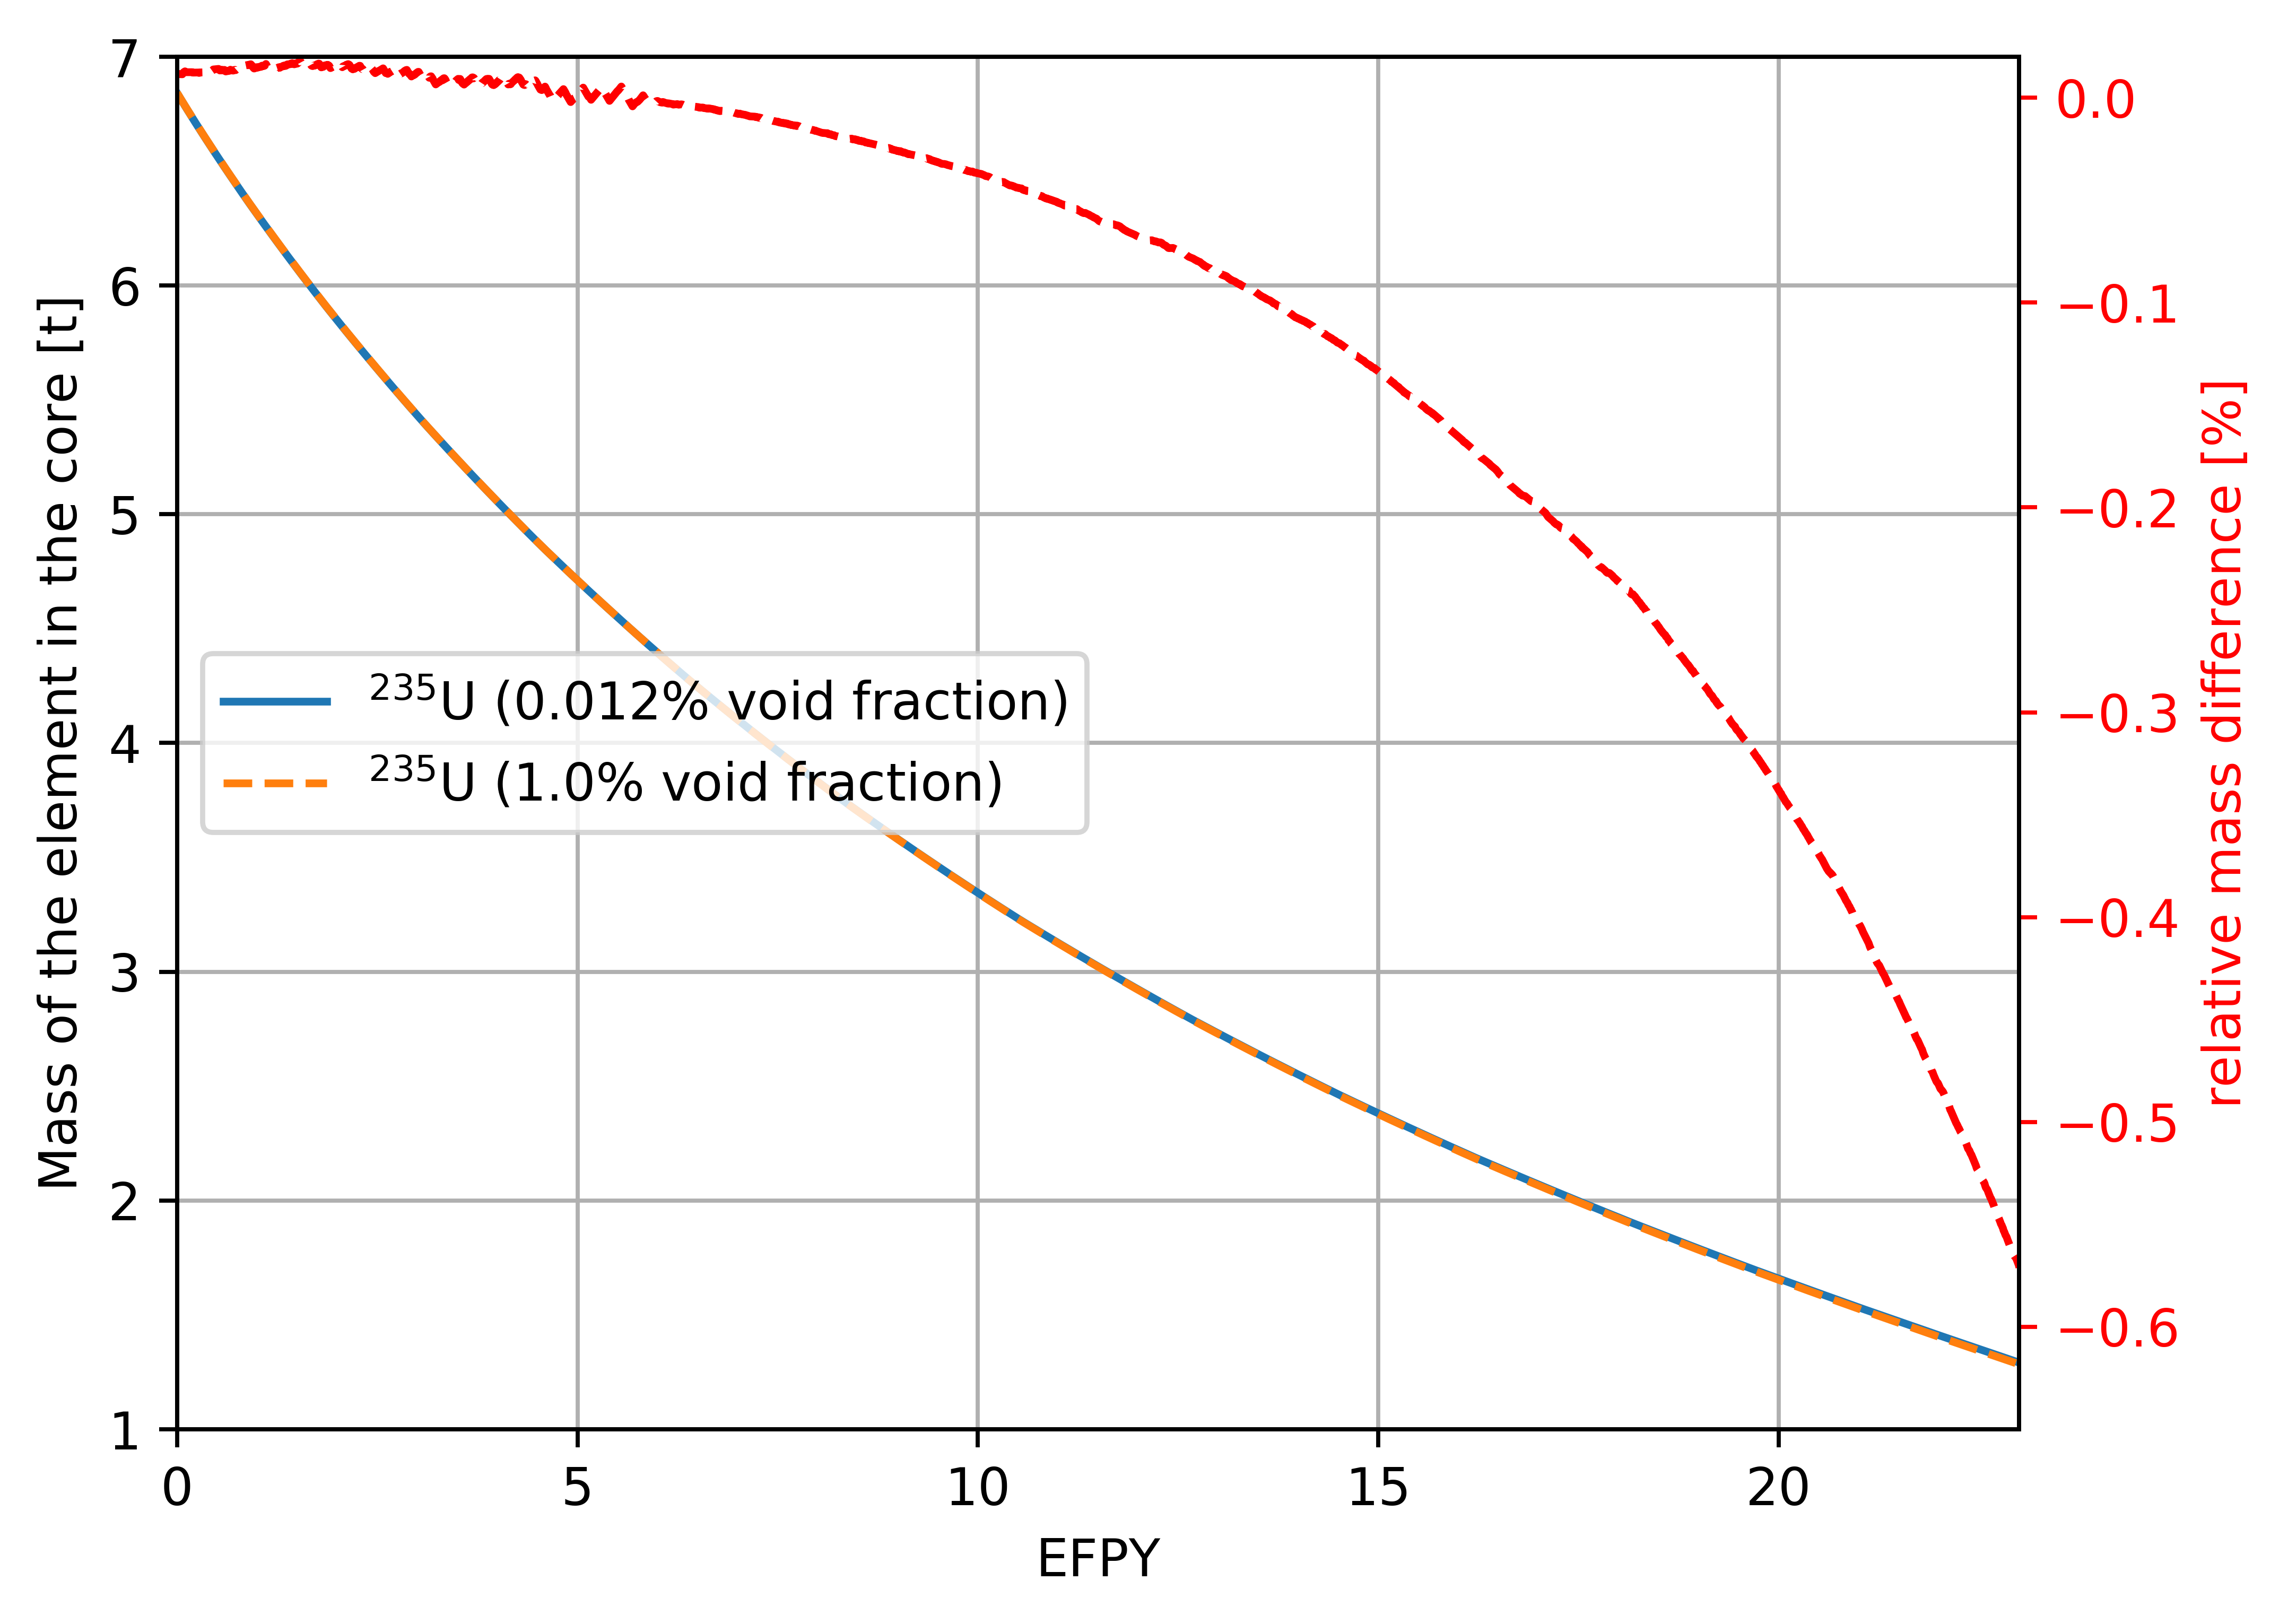
\includegraphics[width=0.8\textwidth]{ch4/eps/u235.png}
	\caption{SaltProc-calculated mass of $^{235}$U in the fuel salt during 
		25 years of operation for $K_L=8.4667$ $mm/s$ compared with less 
		effective noble gas removal.}
	\label{fig:u235-eps-var}
\end{figure}

\begin{figure}[htp!] % replace 't' with 'b' to 
	\centering
	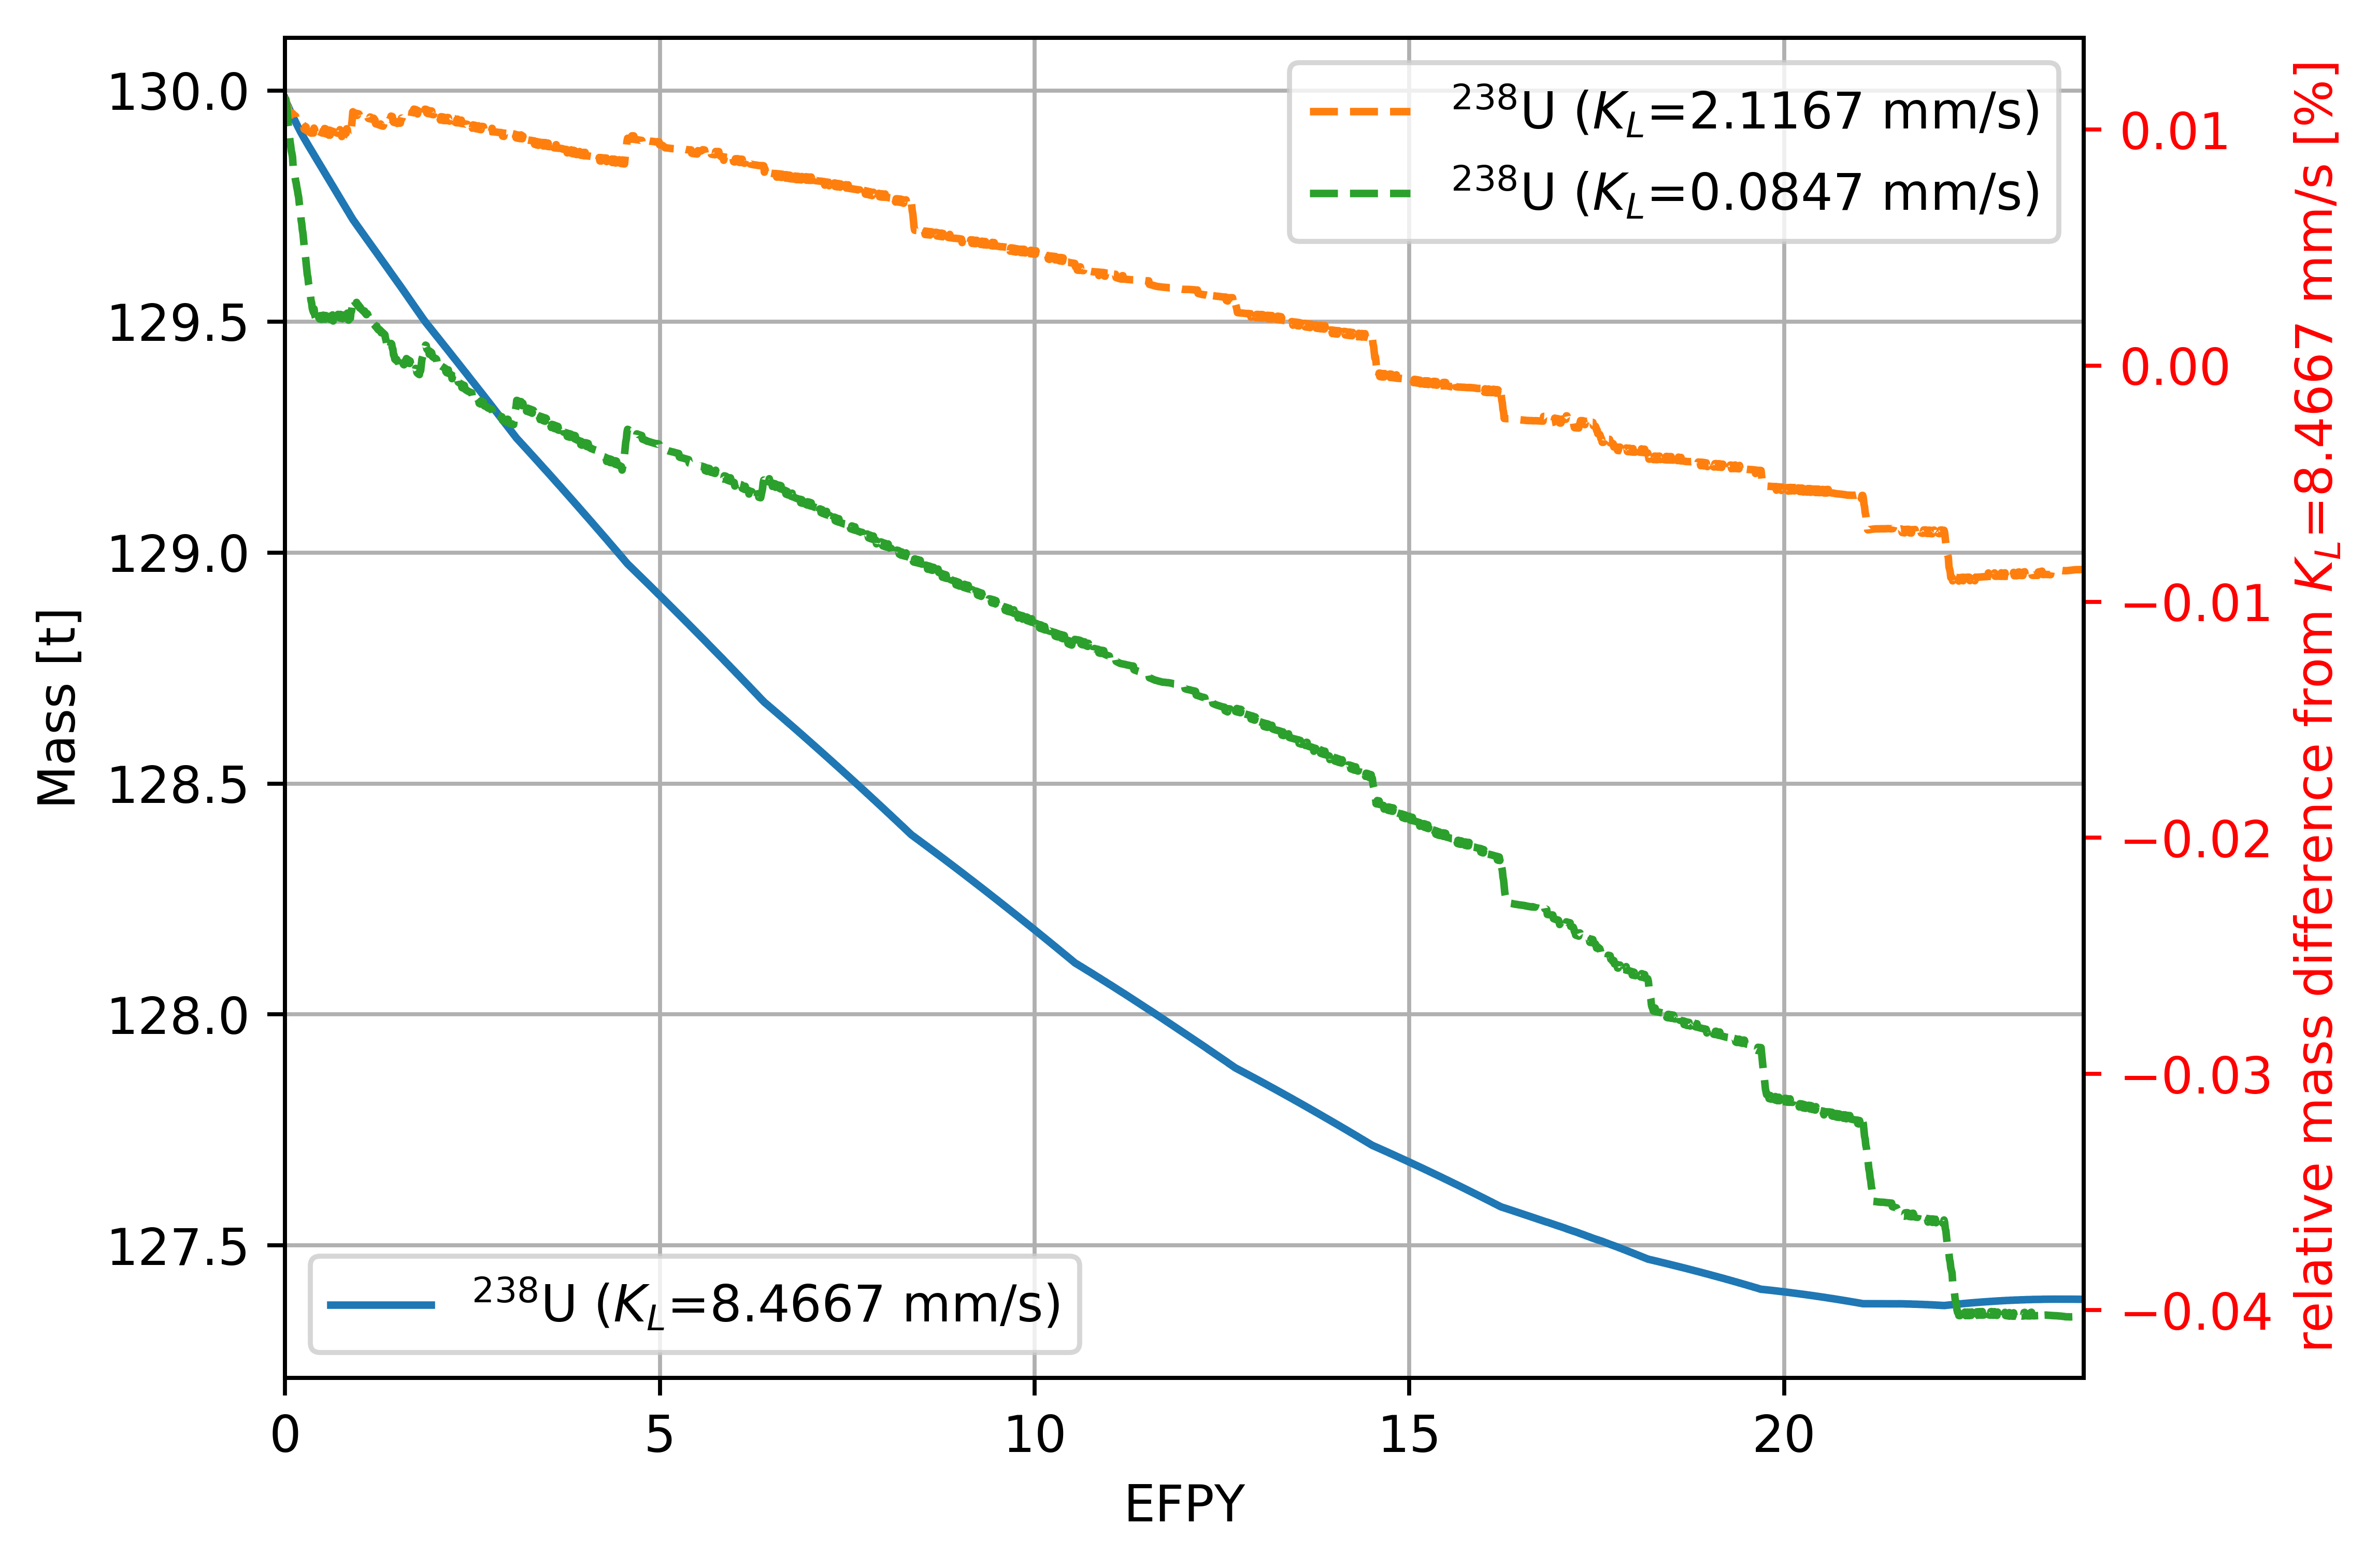
\includegraphics[width=0.88\textwidth]{ch4/eps/u238.png}
	\caption{SaltProc-calculated mass of $^{238}$U in the fuel salt during 
		25 years of operation for $K_L=8.4667$ $mm/s$ compared with less 
		effective noble gas removal.}
	\label{fig:u238-eps-var}
\end{figure}

Differences in the plutonium production between cases with different gas 
removal efficiency are much larger. Over 3\% more $^{239}$Pu is generated in 
the case with $K_L=0.0847$ $mm/s$ than with $K_L=8.4667$ $mm/s$ 
(Figure~\ref{fig:pu239-eps-var}). Larger mass of neutron poison ($^{135}$Xe) 
in the core leads to a harder spectrum (Figure~\ref{fig:spectrum-th-eps-var}) 
which results in a greater rate of destruction of $^{238}$U and a higher 
breeding performance of fissile $^{239}$Pu.
\begin{figure}[hbp!] % replace 't' with 'b' to 
	\centering
	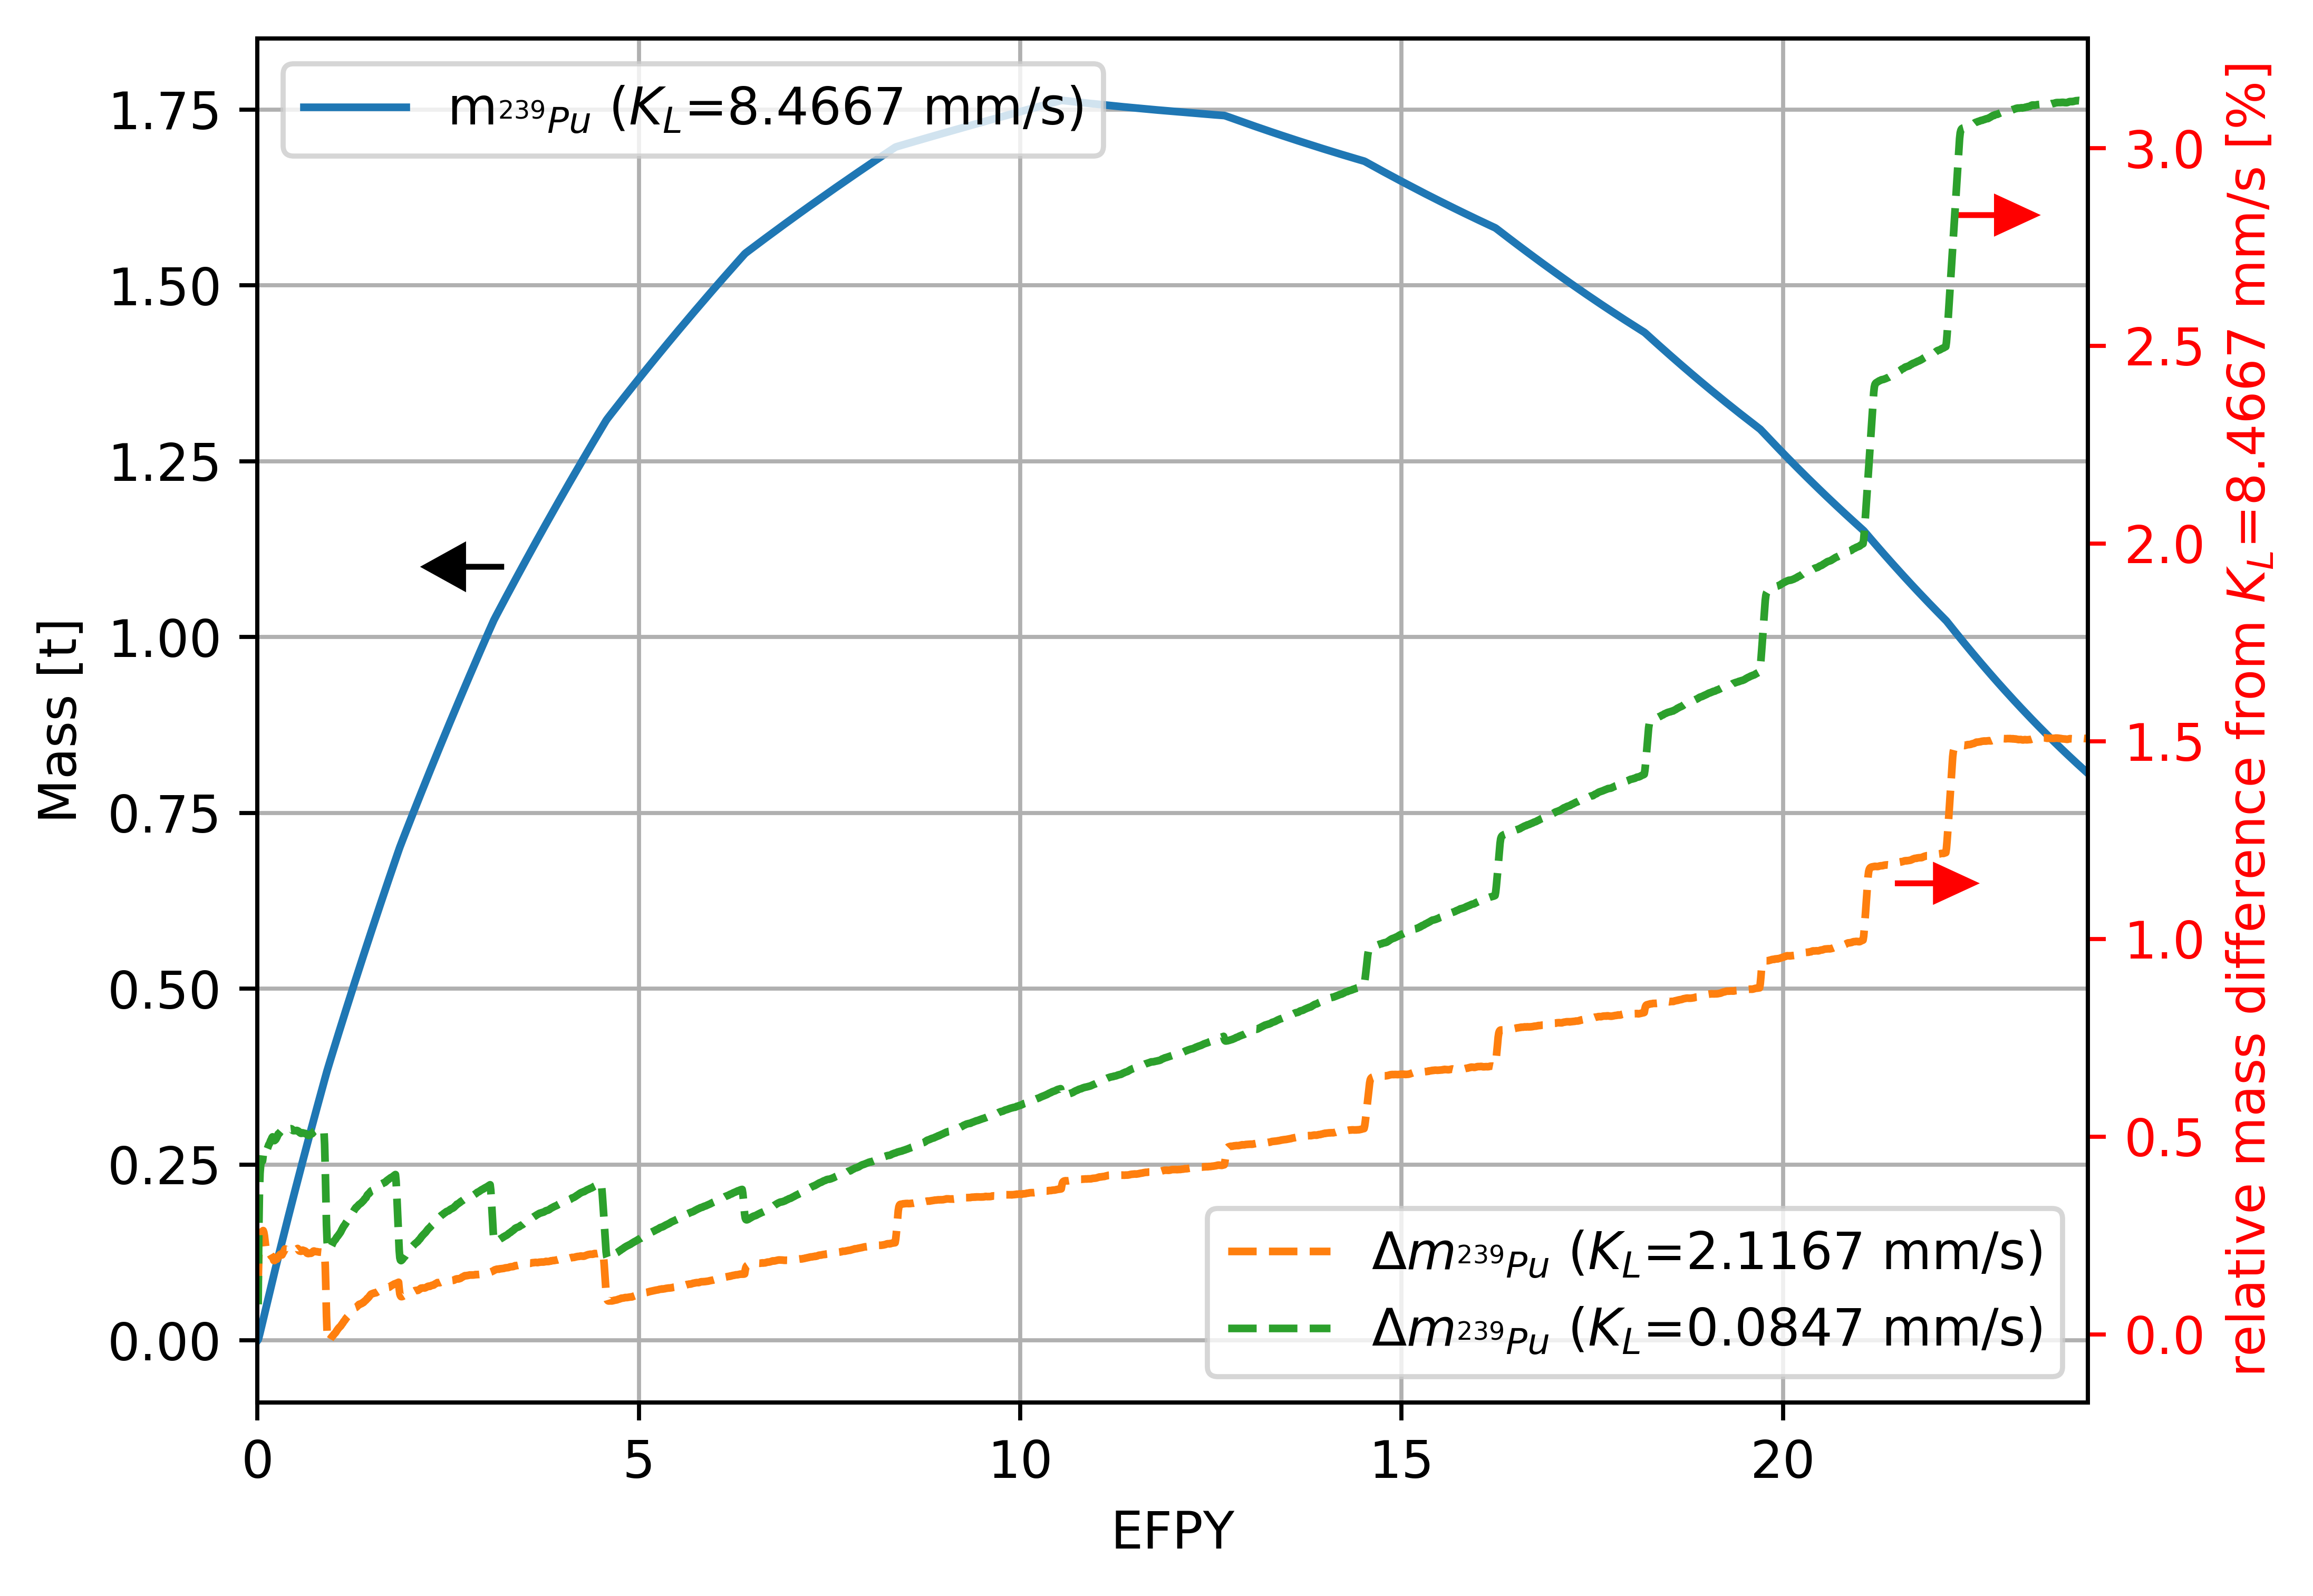
\includegraphics[width=0.8\textwidth]{ch4/eps/pu239.png}
	\caption{SaltProc-calculated mass of $^{239}$Pu in the fuel salt during 
		25 years of operation for $K_L=8.4667$ $mm/s$ (91.5\% of $^{135}$Xe is 
		removed) compared with less effective noble gas removal.}
	\label{fig:pu239-eps-var}
\end{figure}


Figure~\ref{fig:xe135-eps-var} demonstrates $^{135}$Xe mass dynamics in the 
\gls{TAP} core during 25 years of operation for various mass transfer 
coefficients ($K_L$). Jumps in $^{135}$Xe mass every few years are 
representing spectral shift due to moderator rod reconfiguration to shift the 
neutron spectrum from intermediate at the \gls{BOL} to thermal at the 
\gls{EOL}. In contrast, mass of $^{135}$I which is the main direct precursor 
of $^{135}$Xe, is approximately 18 g and stays almost constant over 25 years.

Figure~\ref{fig:xe135-eps-var-zoomes} shows $^{135}$Xe mass at the 
end of each depletion time step before and after performing fuel salt 
reprocessing procedure in SaltProc v1.0. $^{135}$Xe concentration in the core 
after performing \gls{FP} removals behaves as expected and consistent with 
calculated extraction efficiencies in Table~\ref{tab:gas_removal_efficiency}.
Notably, $^{135}$Xe production rate increases during the first 7 years of 
operation and then decreases rapidly to 17 g during  the remaining 17 years as 
the spectrum thermalizes during operation.

\begin{figure}[htp!] % replace 't' with 'b' to 
	\centering
	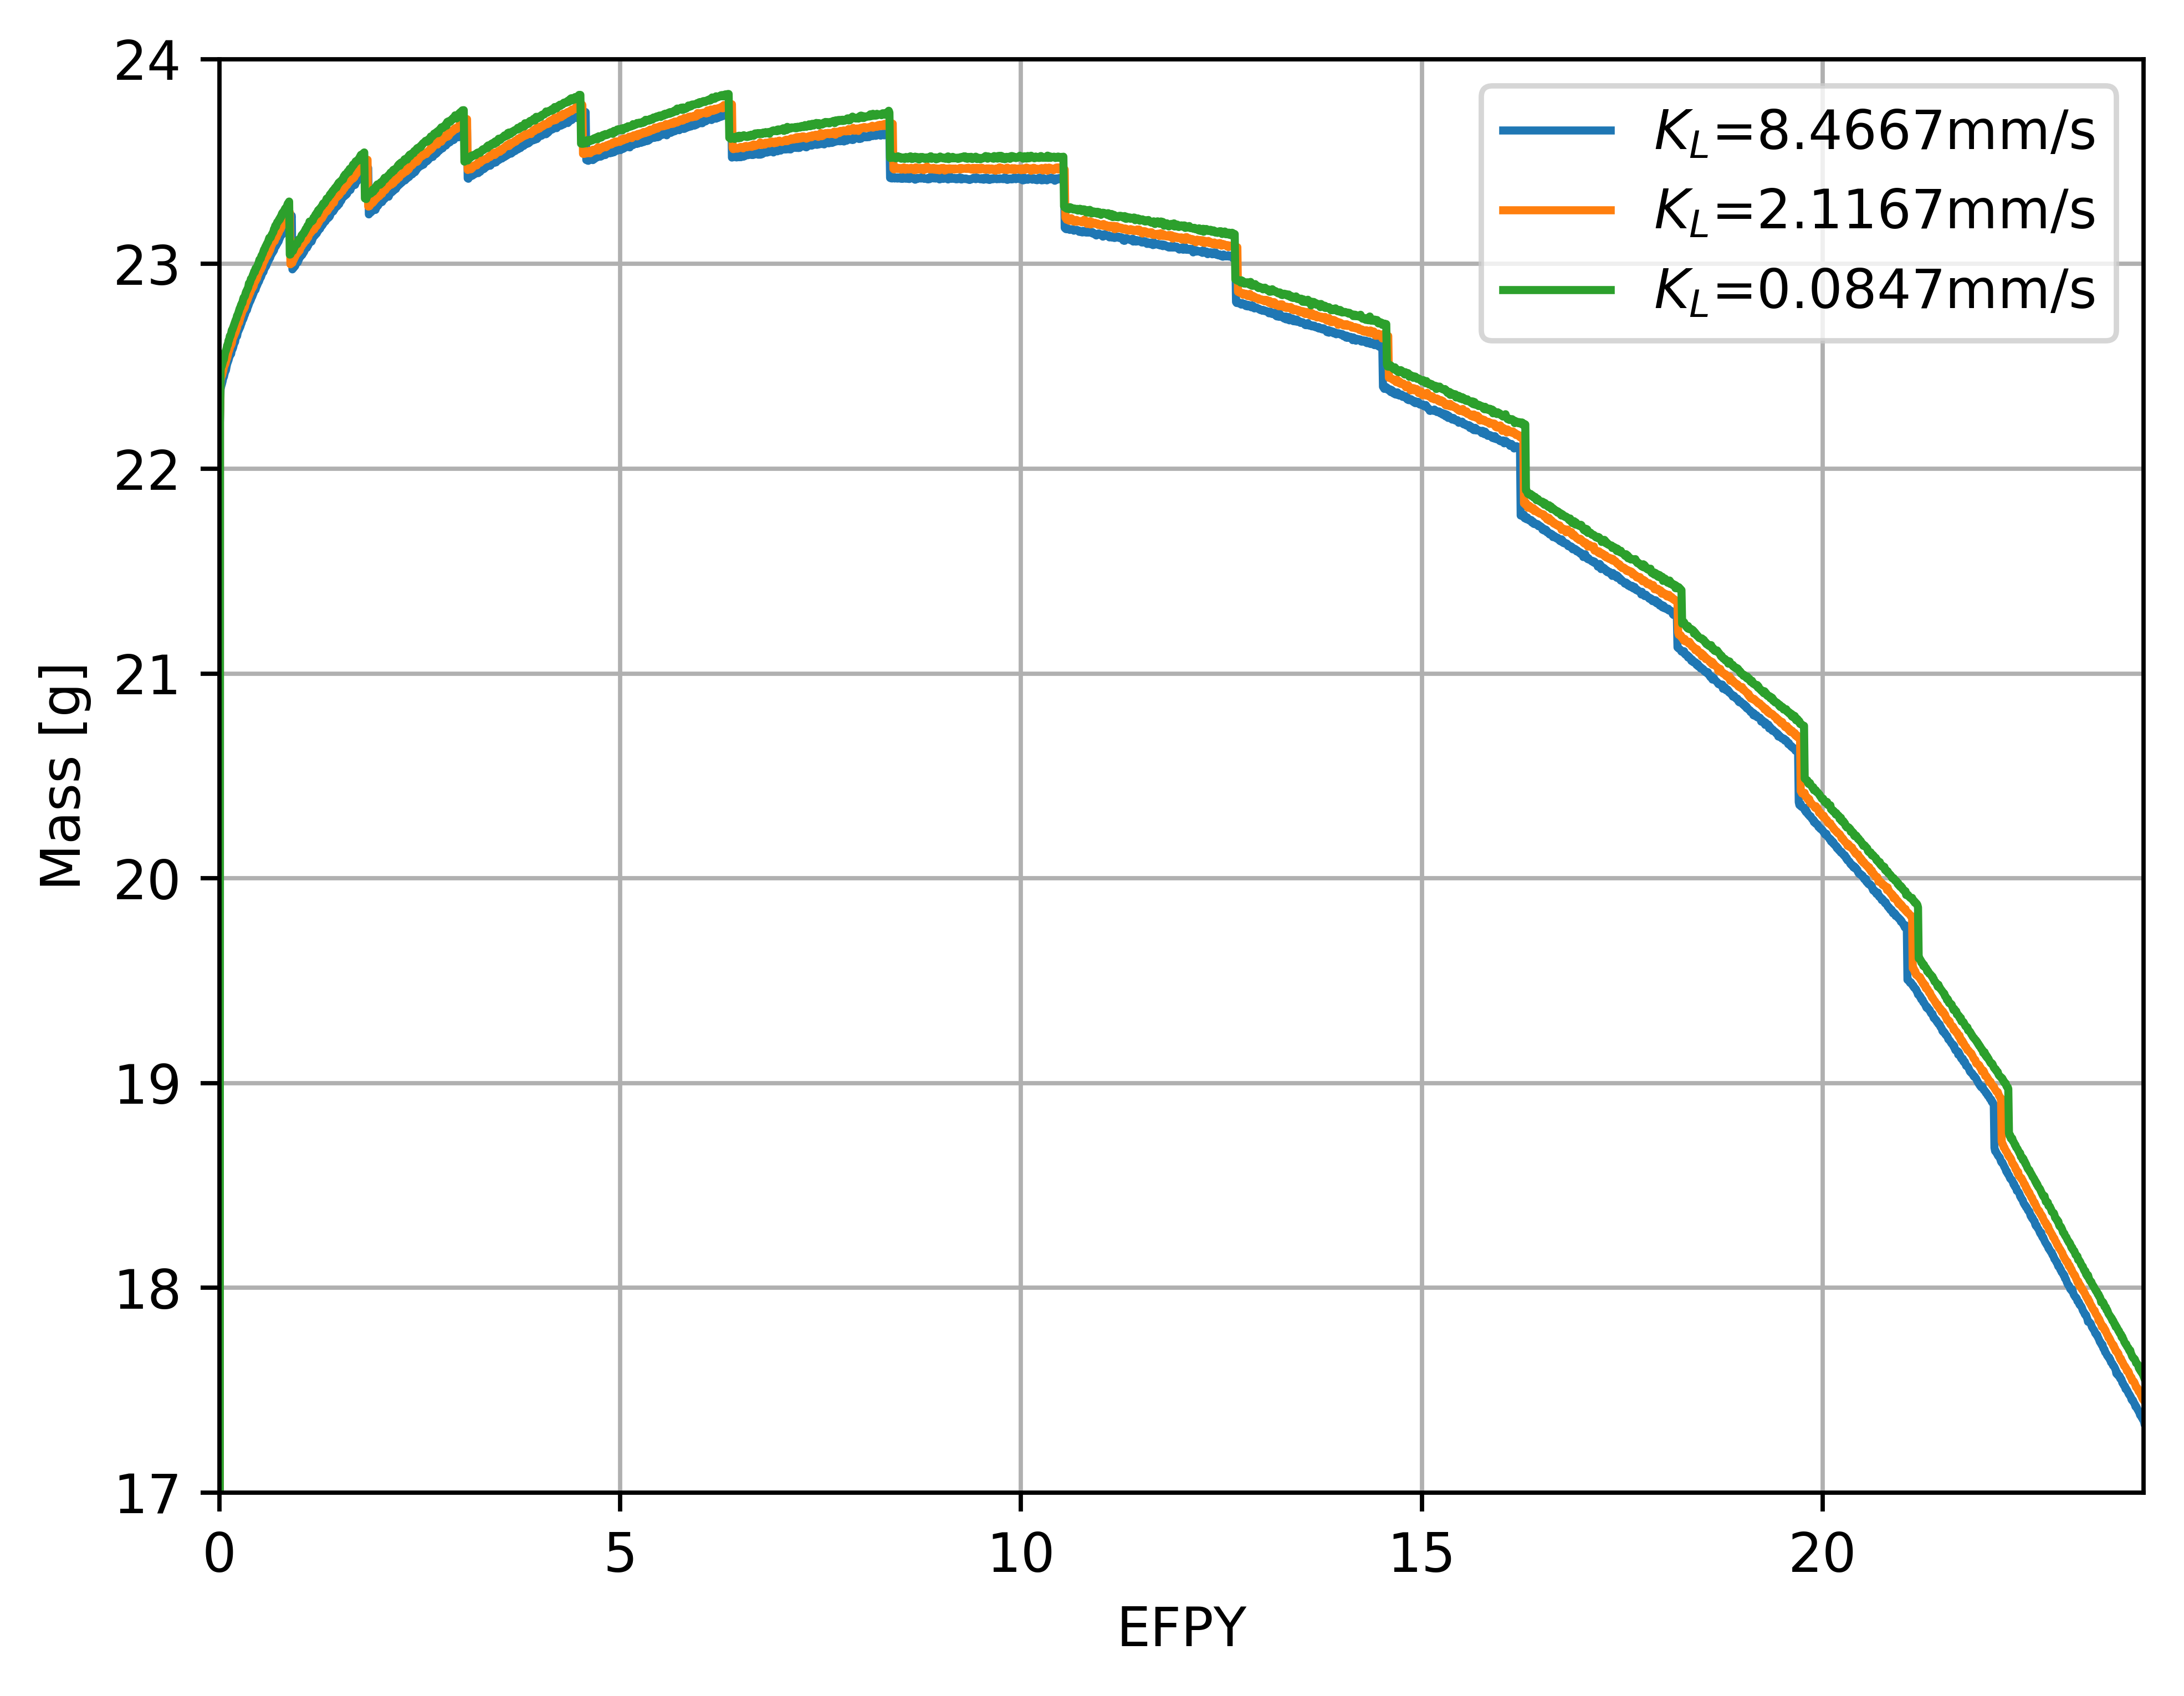
\includegraphics[width=0.85\textwidth]{ch4/eps/xe135.png}
	\caption{SaltProc-calculated mass of $^{135}$Xe in the fuel salt during 
		25 years of operation for the case with realistic removal efficiency 
		of fission product and various mass transfer coefficients ($K_L$).}
	\label{fig:xe135-eps-var}
\end{figure}

I checked correctness of SaltProc v1.0 calculation by comparing the mass of 
$^{135}$Xe to the expected mass after performing removals after each depletion 
step with realistic efficiency (Table~\ref{tab:gas_removal_efficiency}). The 
expected mass of reprocessed isotope is calculated as follows:
\begin{align}
\qquad\qquad\qquad & m_{a} = m_{b} \times  
(1-\epsilon_{m}) \times (1-\epsilon_{es})
\intertext{where}
m_{a} &= \mbox{mass of the isotope after applying removals and feeds} 
\nonumber \\
m_{b} &= \mbox{mass of the isotope right before reprocessing} 
\nonumber \\
\epsilon_{m} &= \mbox{efficiency of the isotope migration to helium bubbles} 
\nonumber \\
\epsilon_{es} &= \mbox{entrainment separator extraction efficiency.} 
\nonumber
\end{align}

This simple check showed that SaltProc-calculated mass of $^{135}$Xe 
(Figure~\ref{fig:xe135-eps-var-zoomes}) matches exactly the expected mass. 
Thus, SaltProc v1.0 extraction module correctly removes target isotopes with 
specified extraction efficiency.

\begin{figure}[htp!] % replace 't' with 'b' to 
	\centering
	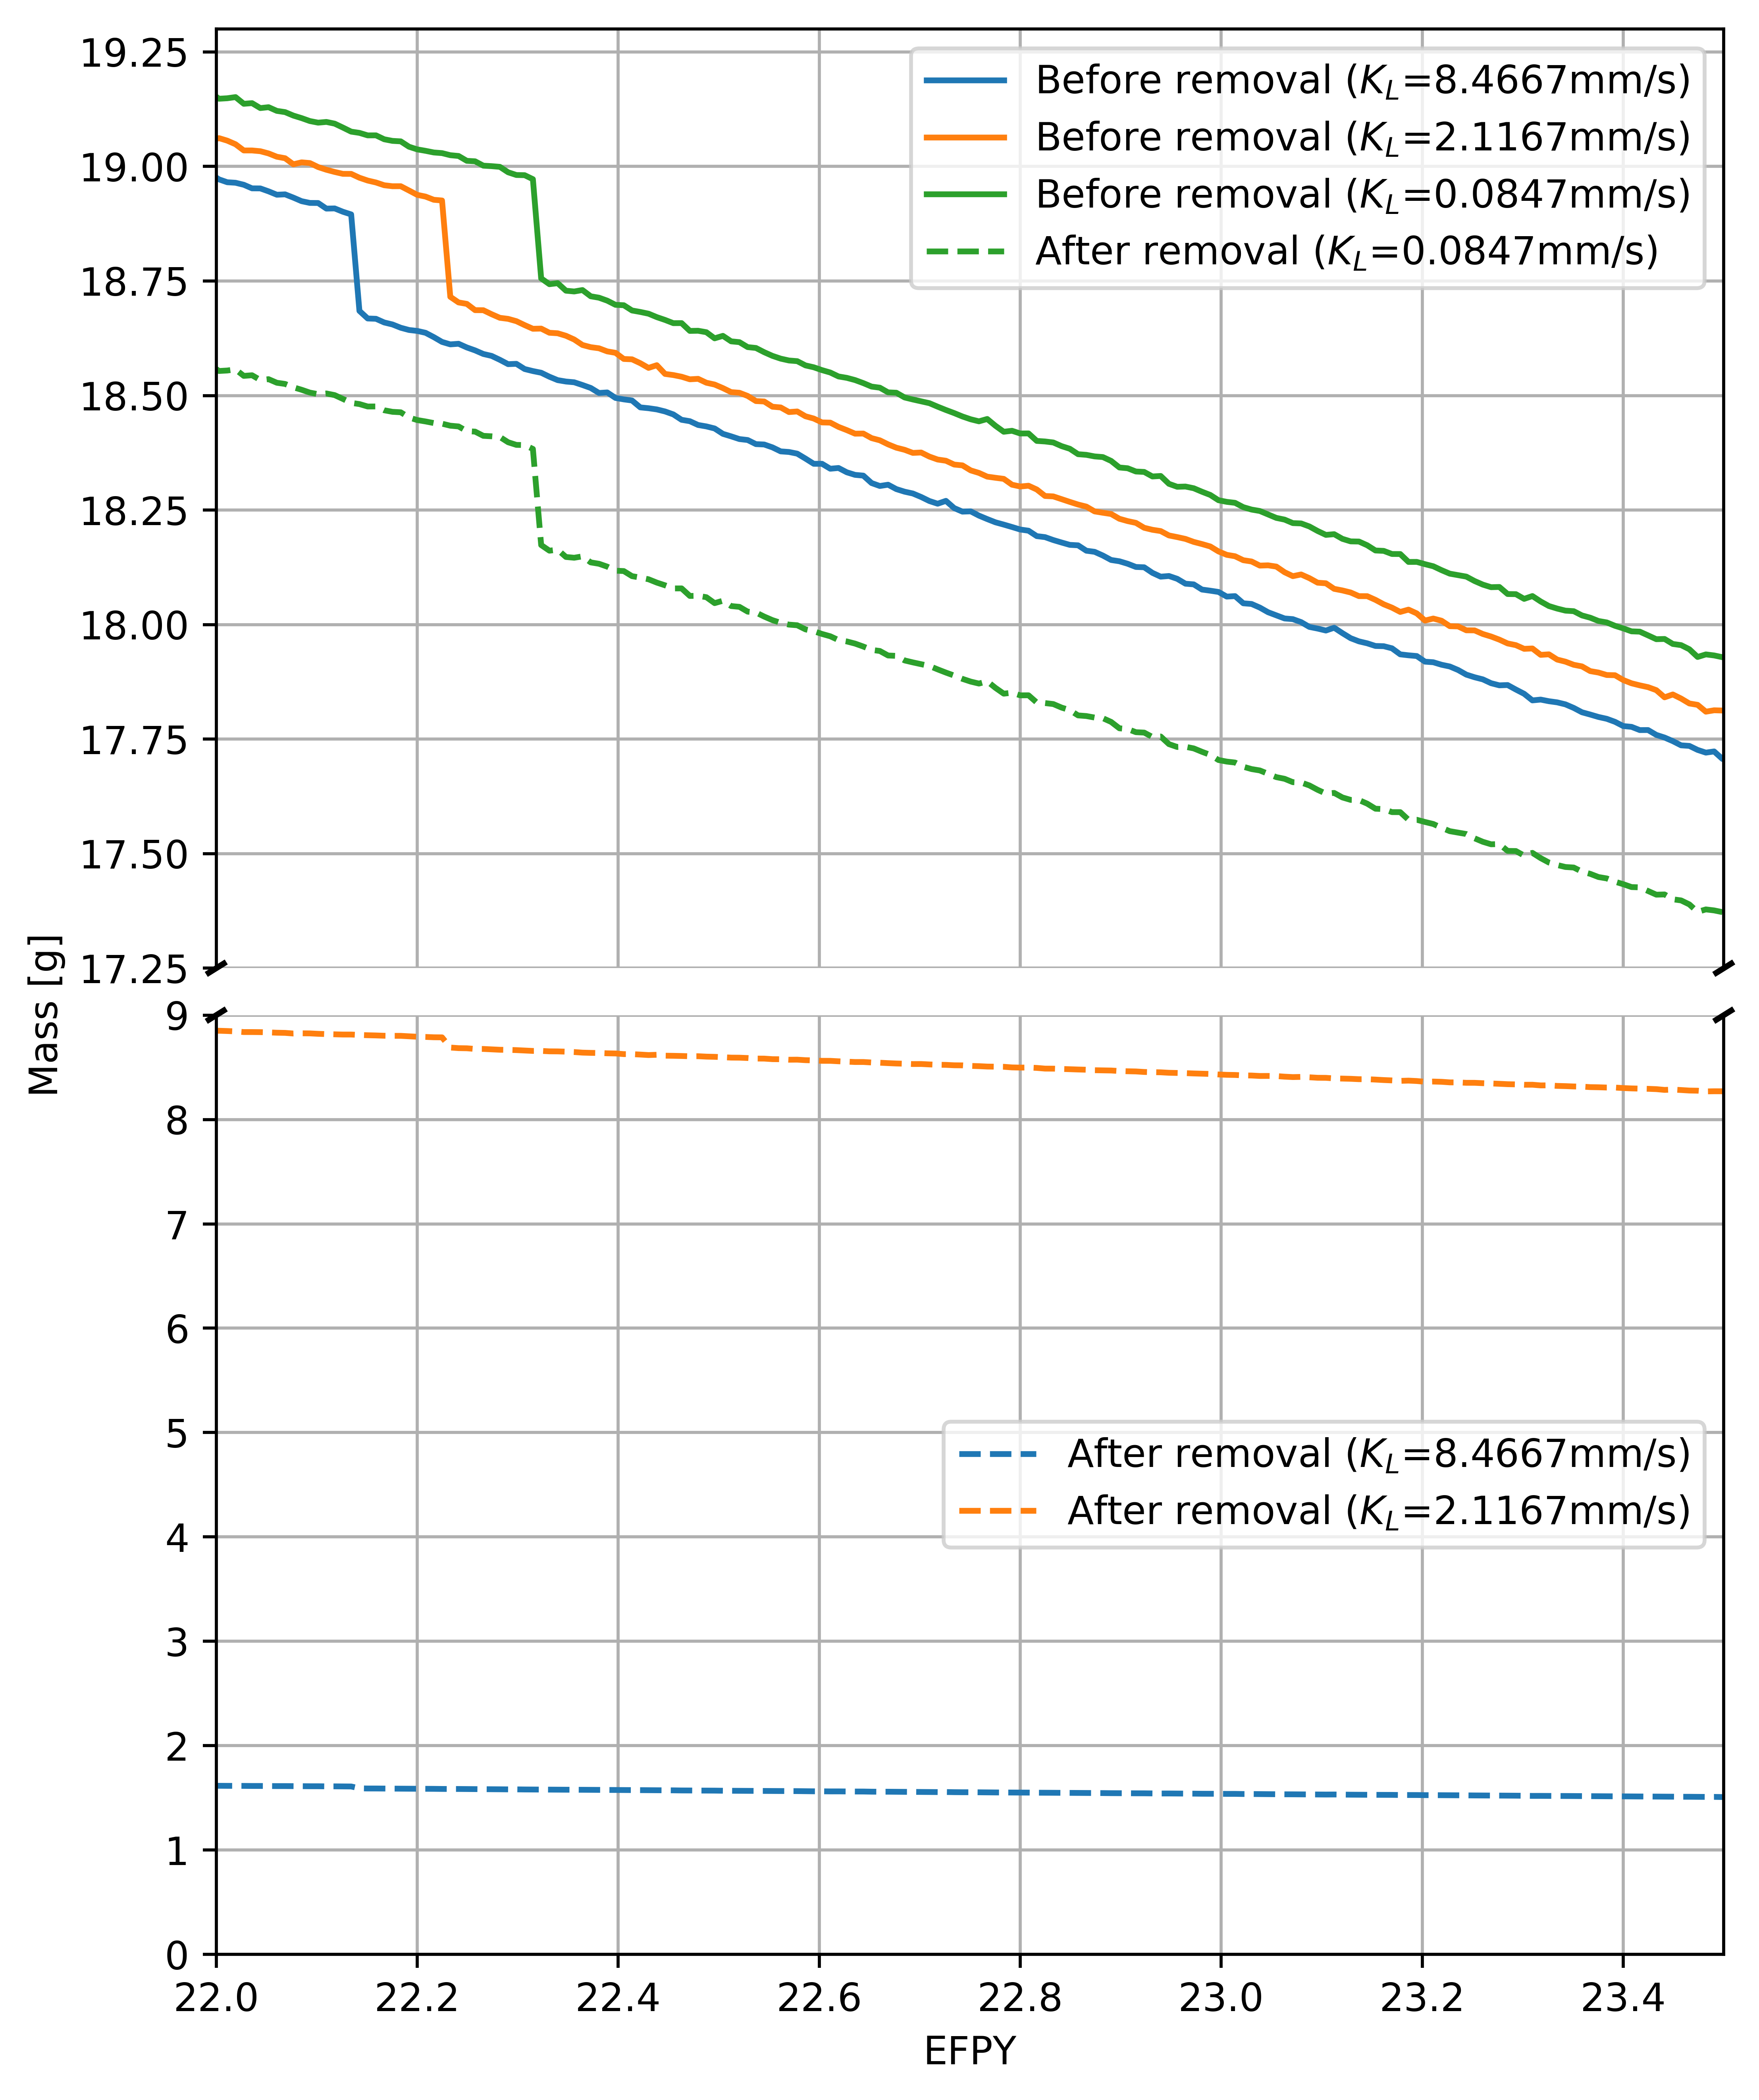
\includegraphics[width=\textwidth]{ch4/eps/xe135_zoomed_3.png}
	\caption{SaltProc-calculated mass of $^{135}$Xe in the fuel salt during 
	last 18 months of operation for various mass transfer coefficients ($K_L$) 
	at the end of each depletion step before and after performing salt 
	treatment.}
	\label{fig:xe135-eps-var-zoomes}
\end{figure}
\FloatBarrier




\section{Concluding remarks}
This chapter demonstrated SaltProc v1.0 capabilities for lifetime-long fuel 
salt depletion simulations applied for the \gls{TAP} \gls{MSR}. 
Section~\ref{sec:tap_design_sum} summarized the \gls{TAP} \gls{MSR} core and 
fuel salt reprocessing system details required to inform SaltProc model. The 
\gls{TAP} \gls{MSR} conceptual design potentially achieves high burnup and 
fuel utilization by shifting the neutron energy spectrum from intermediate at 
startup to thermal at the \gls{EOL}. 
 
Section~\ref{sec:ben-valid} presented lifetime-long depletion simulations with 
SaltProc v1.0. The 25-year simulation with assuming ideal removal efficiency 
(e.g., 100\% of target neutron poison is being removed at the end of each 
depletion step). This validation effort demonstrated good agreement with 
reference ORNL report. Full-core 3D SaltProc/Serpent analysis 
showed that the spectrum hardening over the first 13 years of operation 
produces sufficient amount of fissile plutonium to achieve fuel salt 
burnup of 76.3 MWd/kgU after 22.5 years of operation. SaltProc-calculated 
inventories of major heavy isotopes at the \gls{EOL} are consistent with 
results in the literature. The difference in mass between SaltProc and the 
reference was only 3\% and 4\% for fissile ($^{235}$U, $^{239}$Pu, $^{241}$Pu) 
and non-fissile ($^{236}$U, $^{238}$U, $^{238}$Pu, $^{240}$Pu, $^{242}$Pu) 
isotopes, respectively. Finally, SaltProc-calculated feed rate is 460.8 kg of 
UF$_4$ per year which agrees well with 480 kg/y reported by Betzler \emph{et 
al.} \cite{betzler_assessment_2017-1}

Time step refinement study in Section~\ref{sec:time-refinement} showed that 
accurate uranium isotopic content prediction can be obtained with relatively 
long depletion time step (6- or 12-day). However, significant absolute 
difference in plutonium mass at the \gls{EOL} ($\approx10$ kg for 6-day step) 
could be a safeguards
issue, as this represents more than one significant 
quantity (8 kg) over the reactor lifetime. Overall, to get accurate plutonium 
isotopic content without rising proliferation issues, 3-day depletion time 
step must be used.

Finally, Section~\ref{sec:long-term-real} demonstrated SaltProc v1.0 for 
25-year depletion simulation with realistic, physics-based removal efficiency 
of the noble gas. When identifying reasonable mathematical model for realistic 
gas removal efficiency ($\epsilon$), the liquid phase mass transfer 
coefficient ($K_L$) demonstrated strong correlation with $\epsilon$. Thus, 
SaltProc simulations using different $K_L$ in validity range from 0.0847 to 
8.4667 $mm/s$ (corresponding $^{135}$Xe removal efficiency $\epsilon\in 
[0.031,0.915]$) showed that the larger liquid phase mass transfer coefficient 
and corresponding higher noble gas extraction efficiency provided significant 
neutronics benefit, better fuel utilization, and longer time between shutdowns 
for moderator rod reconfiguration. Notably, the larger mass transfer 
coefficient also provides slightly more thermal neutron spectrum because fewer 
thermal neutrons are absorbed by poisonous \glspl{FP}. In the following 
chapters, results of these realistic depletion simulations will be used for 
short-term transient simulations and safety parameters analysis. 